\chapter{定义项目}

\section{产品愿景与敏捷规划}

\subsection{背景与目的}

\begin{levellist}
    \item \textbf{项目背景} \par
    \hspace{1.6em} 在当前校园外卖服务中，学生订餐主要依赖电话订购或通过零散的第三方平台完成，存在订单管理混乱、信息更新不及时、支付方式单一等问题。日常运营中暴露出以下痛点：
    \begin{levellist}
        \item 业务流程非标准化 \\
        订单处理完全依赖人工记录与传递，存在信息遗漏、重复和错误（如送餐地址、商品规格错误）的高风险，这与软件工程目标中追求的高可靠性与有效性背道而驰。
        \item 角色权责不清晰 \\
        商户无法自主管理商品信息和订单状态，任何变更都需要通过人工沟通，效率低下、成本高昂，违背了模块化与信息隐藏的设计原则。
        \item 用户体验不连贯 \\
        用户无法便捷地查询历史订单或管理个人偏好，缺少系统化的购物车和地址管理，下单流程繁琐，未能满足用户界面设计原则。
        \item 系统扩展性不足 \\
        传统的处理方式无法应对促销活动等带来的订单量激增，缺乏必要的并发处理能力和性能优化，系统稳定性差。
    \end{levellist}

    \hspace{1.6em} 基于对校园外卖市场的深入调研，团队决定从零开始开发"点必达"外卖平台，通过数字化手段实现订单全流程自动化处理，提升用户体验，增强商户自主管理能力。


    \item \textbf{项目核心价值} \par
    \hspace{1.6em} 本项目的核心价值与软件工程的目标（TQCS）紧密对齐，致力于在给定的成本与时间约束下，开发出满足用户需求的高质量软件产品。
    \begin{levellist}
        \item 提升运营效率（成本与进度） \\
        通过自动化订单流程和商户自助管理，减少人工干预，降低运营成本，并确保项目按迭代计划交付。
        \item 改善用户体验（服务与质量） \\
        提供完整、一致的用户界面和流畅的业务流程，在有效性、可靠性、可适应性等方面满足高质量软件的标准。
        \item 构建可扩展架构（可修改性、可追踪性） \\
        采用前后端分离和RESTful接口设计，为未来功能迭代（如AI推荐、多支付方式）奠定技术基础，支持业务的持续增长。
        \item 实现数据驱动（可互操作性） \\
        系统化地收集与分析用户行为数据，为业务决策和后续的再工程提供数据支持。

    \end{levellist}

    \hspace{1.6em} 基于对校园外卖市场的深入调研，团队决定从零开始开发"点必达"外卖平台，通过数字化手段实现订单全流程自动化处理，提升用户体验，增强商户自主管理能力。


    \item \textbf{项目价值与Scrum目标} \par
    \hspace{1.6em}  本项目将严格遵循敏捷软件开发思想，采用Scrum框架作为核心过程模型，并使用与Jira对齐的项目管理工具PingCode进行全过程管理。我们的目标是：通过短周期、高频率的迭代，实现需求的快速响应和可用产品的持续交付，确保在12月15日前完成核心功能的上线。具体包括：
    \begin{levellist}
        \item 快速价值交付 \\
        采用增量开发模式，每个Sprint（2-3周）交付可用的软件增量，确保在12月14日前完成核心功能上线。
        \item 需求灵活响应 \\
        基于MoSCoW优先级法则，优先实现用户注册登录、商铺浏览、下单支付等Must-have核心功能。
        \item 质量持续保障 \\
        通过测试驱动开发和持续集成，每个迭代都产出可部署的软件产品。
        \item 风险主动管理

    \end{levellist}

    \hspace{1.6em} 应用螺旋模型思想，每个迭代周期进行技术风险评估，重点解决支付集成、系统性能等关键技术难点。

    \item \textbf{项目现状}
    \begin{levellist}
        \item 有利条件（优势）
        \begin{levellist}
            \item 清晰的业务域 \\
            外卖业务模式成熟，有大量可参考的成功案例，降低了需求分析的复杂性。
            \item 明确的团队角色 \\
            团队已按Scrum团队模式组建，角色分工明确，具备完成项目所需的各项技能。
            \item 成熟的技术栈 \\
            所选技术栈社区活跃、资料丰富，能有效支撑快速开发。

        \end{levellist}

        \item 不利条件（风险与约束）
        \begin{levellist}
            \item 初始代码为零 \\
            项目完全从零开始，需要进行完整的架构设计、数据库设计和基础组件开发，初始工作量较大。
            \item 外部依赖风险 \\
            支付等关键外部接口的集成存在不确定性，是项目的重要技术风险点。
            \item 紧迫的时间box \\
            仅有三周开发时间，对团队的项目估算和进度管理能力提出了极高要求。

        \end{levellist}
    \end{levellist}


    \item \textbf{项目工作内容}
    \begin{levellist}
        \item 技术架构与基础建设
        \begin{levellist}
            \item 设计并实现基于RESTful风格的API接口规范
            \item 构建完整的用户认证与授权体系，采用Token机制保障系统安全
            \item 设计高并发的系统架构，在关键业务模块引入多线程技术
            \item 实现静态资源管理，采用对象存储服务提升资源访问效率
        \end{levellist}

        \item 核心业务功能开发
        \begin{levellist}
            \item 实现用户端完整的购物流程：注册登录、商铺浏览、商品选择、下单支付
            \item 构建商家端管理功能：店铺申请、商品管理、订单处理、数据统计
            \item 开发管理端审核监管功能：店铺审核、用户管理、运营监控
        \end{levellist}

        \item 系统优化与智能化
        \begin{levellist}
            \item 实施订单超时自动处理等业务流程优化
            \item 探索AI技术在智能推荐、客服问答等场景的应用
            \item 持续进行系统性能优化和用户体验提升
        \end{levellist}

        \item 质量保障与部署运维
        \begin{levellist}
            \item 建立完整的测试体系，包括单元测试、集成测试和系统测试
            \item 实现自动化部署流程，确保系统稳定运行
            \item 建立系统监控和日志分析机制
        \end{levellist}

    \end{levellist}

\end{levellist}


\subsection{项目定义}
\begin{levellist}
    \item \textbf{项目名称} \\
    点必达--外卖平台

    \item \textbf{核心功能定位}
    \begin{levellist}
        \item 顾客端：支持用户注册登录、浏览与搜索商家、查看商家详情和菜单、管理收货地址、下单与支付、查看订单与收藏、接收通知、使用 AI 客服等，完成一整套在线点餐流程。
        \item 商家端：支持商家注册并申请开店、管理商铺信息与商品、查看点赞收藏统计、管理订单（接单 / 拒单 / 完成），实现线上接单经营。
        \item 管理端（支撑功能）：管理员审核商家提交的店铺信息及上线申请，对平台商铺进行管理。
    \end{levellist}

    \item \textbf{目标用户}
    \begin{levellist}
        \item 普通顾客（用户）：需要在线点餐、支付并查看订单状态的人员。
        \item 商家用户：希望在平台上开店、管理商品和订单的食堂档口、校内商铺等。
        \item 平台管理员：负责审核商家资质和店铺信息、保障平台内容与交易安全的运营人员。
    \end{levellist}

\end{levellist}

\newpage


\subsection{迭代周期与Scrum机制}

\begin{levellist}
    \item \textbf{迭代周期规划}

    \begin{longtable}{>{\centering\arraybackslash}m{1cm} >{\centering\arraybackslash}m{3.5cm} >{\centering\arraybackslash}m{4cm} >{\centering\arraybackslash}m{5cm}}

        \caption{迭代周期规划} \label{tab:training}                                                                                                                                                     \\

        \toprule
        \textbf{迭代名称} & \textbf{周期（2025 年）} & \textbf{核心目标}                                 & \textbf{对应高优先级需求（Product Backlog 条目）}                                                               \\
        \midrule
        \endfirsthead

        \multicolumn{4}{c}{{\tablename\ \thetable{} 续表}}                                                                                                                                          \\
        \toprule
        \textbf{迭代名称} & \textbf{周期（2025 年）} & \textbf{核心目标}                                 & \textbf{对应高优先级需求（Product Backlog 条目）}                                                               \\
        \midrule
        \endhead

        \bottomrule
        \endfoot

        Sprint1       & 10.11-10.30         & 构建用户从发现店铺到完成支付的全链路购物体验，支持用户独立完成首次下单。          & US001（用户注册登录）、US002（商铺查询）、US003（商铺详情）、US004（收货地址管理）、US005（购物车支付）、US007（订单查看）、US015（订单推送）            \\
        Sprint2       & 10.31-11.16         & 建立商家入驻和运营管理能力，实现商家从开店到接单的完整工作流，同时增强用户互动功能     & US006（成为商家）、US008（商品管理）、US011（收藏点赞）、US017（商家统计）                                                     \\
        Sprint3       & 11.17-12.7          & 建立管理端，完善平台治理体系，拓展支付方式和用户服务能力，打造更智能、更便捷的电商平台生态 & US009（商家申请审核）、US010（商铺申请审核）、US012（用户管理）、US013（商铺管理）、US014（AI客服）、US016（审核通知）、US018（平台统计）、US019（系统安全） \\
    \end{longtable}


    \item \textbf{Scrum会议机制}
    \begin{levellist}
        \item 迭代启动会：每个迭代开始前 1 天，由Product Owner 讲解当前迭代需完成的Product Backlog（高优先级用户故事）；团队共同拆解用户故事为Sprint Backlog任务，估算工时、明确责任人；确定迭代目标。
        \item 每日站会：每日 19:00-19:15（线上腾讯会议或在图书馆研究箱线下召开），记录昨日进展 、今日计划与遇到的阻碍，由 Scrum Master 整理会议纪要。
        \item 迭代评审会：每个迭代最后 1 天线下召开，由Product Owner 验收已完成用户故事，记录评审结果。
        \item 迭代回顾会：评审会后 1 小时内，团队讨论并记录本次迭代中的亮点与需要改进的地方。
    \end{levellist}

    \item \textbf{任务计划原则}
    \begin{levellist}
        \item 任务拆分：从 Product Backlog 中选取当前迭代需求，拆分为预计工时小于等于8小时的小任务。
        \item 任务跟踪：用 PingCode 建立看板，每个任务标注负责人、预计工时、关联用户故事 ID。
    \end{levellist}
\end{levellist}



\section{项目范围与Product Backlog}

\subsection{项目范围界定}
\begin{enumerate}
    \item 包含范围：用户端（注册 / 登录 / 商铺查询 / 详情查看）、商家端（店铺添加 / 信息编辑）、管理员端（店铺审核 / 用户管理）。
    \item 不包含范围：在线支付、商铺导航、用户评价功能（后续迭代可扩展，当前纳入 P2 需求）。
\end{enumerate}

\subsection{Product Backlog}

\begin{levellist}
    \item \textbf{待办项总览}
    \begin{levellist}
        \item 总故事点：77点
        \item P0（必做核心）：31点
        \item P1（重要功能）：32点
        \item P2（优化增强）：14点
    \end{levellist}

    \item \textbf{详细需求清单}
    \begin{levellist}
        \item P0优先级：系统最小可用版本（MVP）

        \begin{longtable}{>{\centering\arraybackslash}m{2.5cm} >{\centering\arraybackslash}m{1cm} >{\centering\arraybackslash}m{1cm} >{\centering\arraybackslash}m{5cm} >{\centering\arraybackslash}m{1.5cm} >{\centering\arraybackslash}m{1.5cm}}

            \caption{系统最小可用版本需求故事} \label{tab:training}                                                                          \\

            \toprule
            \textbf{用户故事ID} & \textbf{类别} & \textbf{角色} & \textbf{故事描述}                         & \textbf{故事点} & \textbf{Sprint} \\
            \midrule
            \endfirsthead

            \multicolumn{6}{c}{{\tablename\ \thetable{} 续表}}                                                                     \\
            \toprule
            \textbf{用户故事ID} & \textbf{类别} & \textbf{角色} & \textbf{故事描述}                         & \textbf{故事点} & \textbf{Sprint} \\
            \midrule
            \endhead

            \bottomrule
            \endfoot

            US001           & 功能          & 用户          & 作为顾客，我希望通过用户名注册账号并登录系统，以便使用平台的点餐下单功能。 & 5            & Sprint1         \\
            US002           & 功能          & 用户          & 作为顾客，我希望按品类和关键字查询商铺，以便快速找到想要的店。       & 8            & Sprint1         \\
            US003           & 功能          & 用户          & 作为顾客，我希望查看商铺详情和商品列表，以便做出点餐决策。         & 5            & Sprint1         \\
            US004           & 功能          & 用户          & 作为顾客，我希望管理收货地址，以便下单时选择配送地点。           & 5            & Sprint1         \\
            US005           & 功能          & 用户          & 作为顾客，我希望把商品加入购物车并完成在线支付。              & 8            & Sprint1         \\
        \end{longtable}

        \begin{longtable}{>{\centering\arraybackslash}m{2.3cm} >{\centering\arraybackslash}m{8.5cm} >{\centering\arraybackslash}m{4cm}}

            \caption{系统最小可用版本需求故事详述} \label{tab:training}                                                                                                                                                                                                                                                                                                                            \\

            \toprule
            \textbf{用户故事ID} & \textbf{验收标准（AC）}                                                                                                                                                                         & \textbf{关联模块}                                                                                                                                              \\
            \midrule
            \endfirsthead

            \multicolumn{3}{c}{{\tablename\ \thetable{} 续表}}                                                                                                                                                                                                                                                                                                                         \\
            \toprule
            \textbf{用户故事ID} & \textbf{验收标准（AC）}                                                                                                                                                                         & \textbf{关联模块}                                                                                                                                              \\
            \midrule
            \endhead

            \bottomrule
            \endfoot

            US001           & 1）支持用户名+密码注册，校验必填信息格式（用户名未被注册、密码强度≥8位且包含大小写字母和数字，需要确认密码），其它必填信息（头像、姓、名、邮箱、性别）；2）注册后自动拥有顾客权限；3）用户名+密码登录，登录成功后返回JWT token，保持24小时会话，记住我可保持30小时；4）未登录访问受限页面时，前端路由守卫执行跳转；5）密码采用BCrypt加密存储。     & users, authority, user\_authority表Login.vue, Register.vue，/api/auth, /api/register                                                                         \\
            US002           & 1）首页显示分类入口（美食/早餐/跑腿代购/汉堡披萨/甜品饮品/素食简餐/地方小吃/米粉面馆/包子粥铺/炸鸡炸串）；2）首页顶部搜索栏支持关键字模糊匹配（商铺名、商品名）；3）支持按销量、起送费配送费区间筛选；4）搜索结果按评分或销量排序；5）分类入口下方展示销量前三的商家，轮播展示；6）空结果展示友好提示。                               & business表，Index.vue，/api/businesses, /api/business/search，/api/businesses/carousel                                                                         \\
            US003           & 1）商铺详情页展示商家图片、名称、配送费、起送价、商家介绍；2）展示该商铺所有商品列表，包含名称、价格、图片；3）商品信息实时同步商家端修改；4）页面加载时间\textless{}2秒；5）仅已上架商品对顾客可见。                                                                               & business, food表， BusinessInfo.vue， /api/businesses/\{id\}, /api/foods/list                                                                                 \\
            US004           & 1）支持新增、修改、删除配送地址；2）地址信息包含联系人、手机号、详细地址；3）手机号格式需通过前后端双重验证（11位、1开头、第二位\textgreater{}2）；4）订单配送地址选择页面展示所有地址；5）未选择地址时"确认下单"按钮置灰。                                                                & delivery\_address表 ，UserAddress.vue，EditUserAddress.vue，     /api/addresses/getDeliveryAddressById，/api/addresses/updateDeliveryAddress                    \\
            US005           & 1）在商铺详情页选择商品及数量加入购物车；2）商铺详情页底部展示购物车基本信息（所选商品总金额、起送费、配送费）；3）根据所选商品总额是否达起送费显示起送费或去结算按钮；4）购物车页面正确计算商品数量、小计、配送费及订单总价；5）支持购物车商品增删改，数据实时同步；6）下单时首先跳转到选择收货地址页面；7）选择支付方式（支付宝或微信）；8）支付成功跳转到支付成功界面。 & cart, orders, orderdetailet表，Cart.vue, Payment.vue，SuccessfulPayment.vue，BusinessInfo.vue，/api/carts, /api/orders/detail，/api/orders，/api/orders/list/user \\
        \end{longtable}


        \item P1优先级：角色核心能力完善

        \begin{longtable}{>{\centering\arraybackslash}m{2.5cm} >{\centering\arraybackslash}m{1cm} >{\centering\arraybackslash}m{1cm} >{\centering\arraybackslash}m{5cm} >{\centering\arraybackslash}m{1.5cm} >{\centering\arraybackslash}m{1.5cm}}

            \caption{角色核心能力故事} \label{tab:training}                                                                                                                   \\

            \toprule
            \textbf{用户故事ID} & \textbf{类别} & \textbf{角色} & \textbf{故事描述}                                                              & \textbf{故事点} & \textbf{Sprint} \\
            \midrule
            \endfirsthead

            \multicolumn{6}{c}{{\tablename\ \thetable{} 续表}}                                                                                                          \\
            \toprule
            \textbf{用户故事ID} & \textbf{类别} & \textbf{角色} & \textbf{故事描述}                                                              & \textbf{故事点} & \textbf{Sprint} \\
            \midrule
            \endhead

            \bottomrule
            \endfoot

            US006           & 功能          & 顾客/商家       & 作为顾客/商家，我希望申请成为商家/开店。                                                      & 2            & Sprint2         \\
            US007           & 功能          & 顾客/商家       & 作为顾客/商家，我希望查看/管理订单，以便跟踪订单状态。                                               & 5            & Sprint1         \\
            US008           & 功能          & 商家          & 作为商家，我希望管理店铺商品（上架/下架/修改/删除）。                                               & 5            & Sprint2         \\
            US009           & 功能          & 管理员         & 作为管理员，我希望能够审批商家申请。                                                         & 3            & Sprint3         \\
            US010           & 功能          & 管理员         & 作为管理员，我希望能够审批新增商铺的申请。                                                      & 5            & Sprint3         \\
            US011           & 功能          & 用户          & 作为用户，我希望收藏/点赞喜欢的商铺，以便快速访问和表达偏好。                                            & 2            & Sprint2         \\
            US012           & 功能          & 管理员         & {\color[HTML]{RGBA(0, 0, 0, 0.9)} 作为管理员，我希望对用户账号进行启用/禁用管理和搜索，以便维护平台秩序。}    & 5            & Spring3         \\
            US013           & 功能          & 管理员         & {\color[HTML]{RGBA(0, 0, 0, 0.9)} 作为管理员，我希望集中管理所有商家集团及其下属商铺，以便快速维护平台商户信息。} & 5            & Spring3         \\
        \end{longtable}

        \begin{longtable}{>{\centering\arraybackslash}m{2.3cm} >{\centering\arraybackslash}m{4.5cm} >{\centering\arraybackslash}m{7cm}}

            \caption{角色核心能力故事详述} \label{tab:training}                                                                                                                            \\

            \toprule
            \textbf{用户故事ID} & \textbf{验收标准（AC）}                       & \textbf{关联模块}                                                                                            \\
            \midrule
            \endfirsthead

            \multicolumn{3}{c}{{\tablename\ \thetable{} 续表}}                                                                                                                     \\
            \toprule
            \textbf{用户故事ID} & \textbf{验收标准（AC）}                       & \textbf{关联模块}                                                                                            \\
            \midrule
            \endhead

            \bottomrule
            \endfoot

            US006           & 作为顾客/商家，我希望申请成为商家/开店。                   & permission\_application, notification表，ApplyMerchant.vue, AdminAudit.vue，/api/permission/*               \\
            US007           & 作为顾客/商家，我希望查看/管理订单，以便跟踪订单状态。            & orders, orderdetailet表，Order.vue, MerchantOrder.vue，/api/orders/list/*, /api/orders/status               \\
            US008           & 作为商家，我希望管理店铺商品（上架/下架/修改/删除）。            & food表，MerchantFood.vue，/api/foods/status, /api/foods/modifyItem                                          \\
            US009           & 作为管理员，我希望能够审批商家申请。                      & permission\_application表，person表，user\_authority表，AdminAudit.vue，/api/permission/audit                   \\
            US010           & 作为管理员，我希望能够审批新增商铺的申请。                   & business表（status字段），permission\_application表，notification表，AdminShopAudit.vue，/api/permission/audit-shop \\
            US011           & 作为用户，我希望收藏/点赞喜欢的商铺，以便快速访问和表达偏好。         & merchant\_interaction表，BusinessInfo.vue, Favorites.vue，/api/merchant/interaction                         \\
            US012           & 作为管理员，我希望对用户账号进行启用/禁用管理和搜索，以便维护平台秩序。    & person, users表，UserManagement.vue，/api/persons/search, /api/\{username\}/status                          \\
            US013           & 作为管理员，我希望集中管理所有商家集团及其下属商铺，以便快速维护平台商户信息。 & business 表，AdminBusiness.vue，AdminShop.vue/api/businesses ，/api/businesses/\{id\}                        \\
        \end{longtable}

        \newpage

        \item P2优先级：体验优化与增值功能

        \begin{longtable}{>{\centering\arraybackslash}m{2.5cm} >{\centering\arraybackslash}m{1.3cm} >{\centering\arraybackslash}m{1.2cm} >{\centering\arraybackslash}m{5cm} >{\centering\arraybackslash}m{1.3cm} >{\centering\arraybackslash}m{1.2cm}}

            \caption{体验优化与增值功能故事} \label{tab:training}                                                                      \\

            \toprule
            \textbf{用户故事ID} & \textbf{类别} & \textbf{角色} & \textbf{故事描述}                    & \textbf{故事点} & \textbf{Sprint} \\
            \midrule
            \endfirsthead

            \multicolumn{6}{c}{{\tablename\ \thetable{} 续表}}                                                                \\
            \toprule
            \textbf{用户故事ID} & \textbf{类别} & \textbf{角色} & \textbf{故事描述}                    & \textbf{故事点} & \textbf{Sprint} \\
            \midrule
            \endhead

            \bottomrule
            \endfoot

            US014           & 功能          & 用户          & 作为顾客，我希望通过AI智能助手咨询商家或菜品信息。       & 5            & Sprint3         \\
            US015           & 功能          & 用户/商家       & 作为交易方，我希望订单状态变化能实时推送到我，以便及时跟进履约  & 3            & Sprint1         \\
            US016           & 功能          & 申请人（顾客/商家）  & 作为申请人，我希望审核结果能第一时间通知我，以便及时开展后续业务 & 1            & Spring3         \\
            US017           & 功能          & 商家          & 作为商家，我希望实时了解本店经营人气，以便优化运营策略。     & 1            & Sprint2         \\
            US018           & 功能          & 管理员         & 作为管理员，我希望掌握平台整体经营指标，以便快速决策。      & 1            & Spring3         \\
            US019           & 非功能         & 系统          & 作为系统，我需要保证用户数据安全与接口稳定。           & 3            & Sprint3         \\
        \end{longtable}

        \begin{longtable}{>{\centering\arraybackslash}m{2.3cm} >{\centering\arraybackslash}m{7.5cm} >{\centering\arraybackslash}m{4cm}}

            \caption{体验优化与增值功能故事详述} \label{tab:training}                                                                                                                                                                                                                            \\

            \toprule
            \textbf{用户故事ID} & \textbf{验收标准（AC）}                                                                                                                                               & \textbf{关联模块}                                                                       \\
            \midrule
            \endfirsthead

            \multicolumn{3}{c}{{\tablename\ \thetable{} 续表}}                                                                                                                                                                                                                        \\
            \toprule
            \textbf{用户故事ID} & \textbf{验收标准（AC）}                                                                                                                                               & \textbf{关联模块}                                                                       \\
            \midrule
            \endhead

            \bottomrule
            \endfoot

            US014           & 1）首页右下角悬浮AI助手入口；2）支持自然语言提问，识别商家咨询/商品推荐意图；3）调用DeepSeek API返回回答，响应时间\textless{}3秒；4）对话历史持久化存储，支持查看历史记录；5）网络失败时显示友好提示并重试。                                          & ai\_chat\_history表，AIChat.vue，/api/merchant/interaction                             \\
            US015           & 1）顾客下单成功后，商家端 1s 内收到 WebSocket 类型=order\_pending 推送；2）商家接单/拒单/完成时，顾客端 1s 内收到对应状态推送；3）消息体包含 orderId、状态、变更时间，可点击查看订单详情；4）未读订单消息在导航栏红点提示，已读立即消失；5）网络闪断时自动重连，消息不丢失。 & notification表，WebSocket，Message.vue，/api/notifications                              \\
            US016           & 1）提交"成为商家"或"新增商铺"申请后，系统返回"审核中"提示；2）管理员点击"批准/拒绝"后，申请人 1s 内收到站内通知（类型=audit\_result）；3）通知标题固定为"审核结果"，正文含审核类型与结论；4）未读审核消息红点计数，已读后消失；5）审核通过时，通知栏增加"立即去开店/切换身份"快捷入口。  & permission\_application表，notification表，WebSocket，Message.vue，/api/permission/audit* \\
            US017           & 1）商家端我的页面展示该商家所有商铺的点赞数、收藏数、综合评分（点赞与收藏加权归一化）。                                                                                                                    & merchant\_interaction表，business表，MerchantStats.vue ，/api/merchant/interaction/stats \\
            US018           & 1）管理端首页顶部展示总用户数、总店铺数、总营业额（元）三合一卡片。                                                                                                                              & user表 ，business表，orders表，AdminDashboard.vue，/api/admin/count*                       \\
            US019           & 1）密码采用BCrypt加密存储；2）所有接口采用JWT认证，无token请求返回401；3）前端请求/响应拦截器处理异常，网络错误重试3次；4）手机号格式前后端双重验证；5）SQL注入/XSS防护通过率100\%（安全测试用例）。                                            & SpringSecurity配置，axios拦截器，/api/auth拦截逻辑                                             \\
        \end{longtable}



    \end{levellist}

    \item \textbf{需求优先级说明}
    \begin{levellist}
        \item \textbf{P0（必做核心）：} 支撑MVP核心流程，缺失则系统不可用。包括用户注册登录、商铺浏览搜索、购物车下单、商铺详情查看，构成"浏览-加购-支付"最小闭环。
        \item \textbf{P1（重要功能）：} 完善角色核心能力，缺失则业务不完整。包括地址管理、商家入驻审核、订单状态管理、商品管理，确保"顾客-商家-管理员"三端权责清晰。
        \item \textbf{P2（优化增强）：} 提升体验或增值功能，缺失不影响核心使用。包括收藏点赞、AI客服、实时通知、数据统计看板，属于差异化竞争力功能。
    \end{levellist}

\end{levellist}

\section{技术架构与风险应对}

\subsection{技术栈选型}

\begin{levellist}
    \item \textbf{前端}
    \begin{itemize}
        \item Vue3
        \item HTML、CSS、JavaScript
    \end{itemize}

    \item \textbf{后端}
    \begin{levellist}
        \item 框架及配置
        \begin{itemize}
            \item SpringBoot 3.4.6
            \item Maven
            \item Mybatis 3.0.4
            \item JDK 17
        \end{itemize}

        \item 数据库
        \begin{itemize}
            \item MySQL
        \end{itemize}
    \end{levellist}

    \item \textbf{运维}
    \begin{itemize}
        \item docker 使用容器化管理部署
        \item Ubuntu 22.04 操作系统
    \end{itemize}

\end{levellist}


\subsection{风险与敏捷应对}

本项目在开发过程中可能面临技术选型不确定、需求变更频繁以及进度紧迫等挑战。主要风险概览如下：

\begin{longtable}{>{\centering\arraybackslash}m{2cm} >{\centering\arraybackslash}m{6cm} >{\centering\arraybackslash}m{6cm}}

    \caption{风险概览} \label{tab:training}                            \\

    \toprule
    \textbf{风险类别} & \textbf{潜在风险描述} & \textbf{对应的敏捷应对措施 }          \\
    \midrule
    \endfirsthead

    \multicolumn{3}{c}{{\tablename\ \thetable{} 续表}}               \\
    \toprule
    \textbf{风险类别} & \textbf{潜在风险描述} & \textbf{对应的敏捷应对措施 }          \\
    \midrule
    \endhead

    \bottomrule
    \endfoot

    需求风险          & 需求理解偏差、功能范围蔓延   & 迭代回顾会 、用户故事地图                \\
    技术风险          & 新技术学习成本高、性能瓶颈   & 技术预研 (Spike)、自动化测试覆盖         \\
    进度风险          & 任务预估偏差、DDL临近    & 燃尽图监控、MoSCoW 优先级排序法          \\
    沟通风险          & 成员进度不同步、接口文档滞后  & 每日站会、Swagger/Apifox 接口文档自动同步 \\
\end{longtable}

鉴于此，项目组采用 敏捷开发模式（Scrum） 进行管理，通过迭代和反馈机制，在宏观层面将风险降至最低。以下是针对本项目主要风险的识别及敏捷应对策略：

\begin{levellist}
    \item \textbf{需求变更风险}
    \begin{itemize}
        \item \textbf{风险描述：} 由于项目初期用户需求尚不完全明确，或在开发过程中客户对功能提出新的想法，可能导致频繁的需求变更和返工。
        \item \textbf{敏捷应对：}
              \begin{itemize}
                  \item \textbf{短周期迭代：} 将开发周期划分为若干个短 Sprint（3阶段），每个 Sprint 结束时交付可运行的软件增量，及时获取反馈。
                  \item \textbf{Product Backlog 梳理：} 定期进行需求梳理会议，根据优先级调整待办事项列表，拥抱变化，而非抗拒变化。
              \end{itemize}
    \end{itemize}

    \item \textbf{技术与集成风险}
    \begin{itemize}
        \item \textbf{风险描述：} 团队成员可能对部分新引入的技术栈（ Vue3, mybatis）不够熟练，或在模块集成时遇到未预期的接口冲突。
        \item \textbf{敏捷应对：}
              \begin{itemize}
                  \item \textbf{技术探针 (Spike)：}  在正式开发前，安排专门的 Story 用于技术调研和原型验证，提前扫除技术盲点。
                  \item \textbf{持续集成：} 引入自动化构建和测试流程，确保代码提交即测试，尽早发现集成错误。
              \end{itemize}
    \end{itemize}

    \item \textbf{进度与时间风险}
    \begin{itemize}
        \item \textbf{风险描述：} 项目预留时间与正常课程安排存在重合，团队成员时间碎片化，可能导致关键节点延期。
        \item \textbf{敏捷应对：}
              \begin{itemize}
                  \item \textbf{MVP 策略：} 优先开发 最小可行性产品 (MVP) 的核心功能，确保在Deadline前至少有一个可演示的基础版本。
                  \item \textbf{每日站会：} 通过每日短会（线上或线下）同步进度，及时暴露阻碍，避免问题积压到最后一周。
              \end{itemize}
    \end{itemize}

    \item \textbf{人员协作风险}
    \begin{itemize}
        \item \textbf{风险描述：} 团队成员分工可能出现边界模糊，或者因沟通不畅导致的代码风格不一致、接口定义误解。
        \item \textbf{敏捷应对：}
              \begin{itemize}
                  \item \textbf{代码评审：} 在合并代码前强制进行 Review，保证代码质量和风格统一。
                  \item \textbf{结对编程：} 针对攻坚难点采用结对编程，促进知识共享，防止单点故障（即某人请假导致项目停摆）。
              \end{itemize}
    \end{itemize}

\end{levellist}


\newpage

\section{数据库设计}

\subsection{数据库概述}
本数据库设计基于支撑系统MVP核心闭环、完善各角色核心能力及提供体验优化功能的用户故事需求，遵循“第三范式”，确保数据冗余最小，同时支撑。

\subsection{数据库设计}

\begin{enumerate}

    \item \textbf{总览设计}

          \begin{longtable}{>{\centering\arraybackslash}m{0.5cm} >{\centering\arraybackslash}m{5cm} >{\centering\arraybackslash}m{3.5cm} >{\centering\arraybackslash}m{4.5cm}}

              \caption{数据库表设计总览} \label{tab:training}                                  \\

              \toprule
              \textbf{NO} & \textbf{数据库表名}          & \textbf{中文概括名} & \textbf{说明}     \\
              \midrule
              \endfirsthead

              \multicolumn{4}{c}{{\tablename\ \thetable{} 续表}}                         \\
              \toprule
              \textbf{NO} & \textbf{数据库表名}          & \textbf{中文概括名} & \textbf{说明}     \\
              \midrule
              \endhead

              \bottomrule
              \endfoot

              1           & ai\_chat\_history       & AI对话历史表        & 接入智能体对话历史       \\
              2           & authority               & 权限类型表          & 用户可以拥有的权限类型名    \\
              3           & business                & 商铺表            & 商铺信息            \\
              4           & cart                    & 购物车表           & 用户购物车商品信息       \\
              5           & delivery\_address       & 配送地址表          & 用户配送地址信息        \\
              6           & food                    & 商品表            & 商铺中的商品信息        \\
              7           & merchant\_interaction   & 用户对商铺动作表       & 用户点赞/收藏商铺记录     \\
              8           & notification            & 消息通知表          & 消息通知记录          \\
              9           & orderdetailet           & 订单详情表          & 订单中包含的商品信息      \\
              10          & orders                  & 订单表            & 订单信息            \\
              11          & permission\_application & 权限申请表          & 用户权限申请记录        \\
              12          & person                  & 自然人信息表         & 自然人(商家/顾客用户)的信息 \\
              13          & user\_authority         & 用户权限表          & 记录用户拥有的权限       \\
              14          & users                   & 用户表            & 用户(登录)信息        \\
          \end{longtable}


          \begin{longtable}{>{\centering\arraybackslash}m{2cm} >{\centering\arraybackslash}m{4cm} >{\centering\arraybackslash}m{6.5cm}}

              \caption{数据库约束说明} \label{tab:training}           \\

              \toprule
              \textbf{标识} & \textbf{英文}    & \textbf{解释}       \\
              \midrule
              \endfirsthead

              \multicolumn{3}{c}{{\tablename\ \thetable{} 续表}} \\
              \toprule
              \textbf{标识} & \textbf{英文}    & \textbf{解释}       \\
              \midrule
              \endhead

              \bottomrule
              \endfoot


              PK          & primary key    & 主键                \\
              FK          & foreign key    & 外键                \\
              NN          & not null       & 非空                \\
              UQ          & unique         & 唯一索引              \\
              AI          & auto increment & 自增长列              \\
              DEL         & delete         & 逻辑删除标记0-正常 1-删除   \\
          \end{longtable}


    \item \textbf{表设计}

          \begin{itemize}
              \item ai\_chat\_history (AI对话历史表)

                    \begin{longtable}{>{\centering\arraybackslash}m{0.2cm} >{\centering\arraybackslash}m{2.2cm} >{\centering\arraybackslash}m{2.1cm} >{\centering\arraybackslash}m{1.5cm} >{\centering\arraybackslash}m{1.5cm} >{\centering\arraybackslash}m{2cm} >{\centering\arraybackslash}m{2.5cm}}

                        \caption{AI对话历史表} \label{tab:training}                                                                                     \\

                        \toprule
                        \textbf{NO} & \textbf{Field } & \textbf{Type } & \textbf{Size} & \textbf{Default} & \textbf{Constraint} & \textbf{Comment} \\
                        \midrule
                        \endfirsthead

                        \multicolumn{7}{c}{{\tablename\ \thetable{} 续表}}                                                                           \\
                        \toprule
                        \textbf{NO} & \textbf{Field } & \textbf{Type } & \textbf{Size} & \textbf{Default} & \textbf{Constraint} & \textbf{Comment} \\
                        \midrule
                        \endhead

                        \bottomrule
                        \endfoot

                        1           & id              & bigint         & ~             & ~                & NN PK AI            & 对话id             \\
                        2           & create\_time    & timestamp      & ~             & ~                & ~                   & 创建时间             \\
                        3           & creator         & bigint         & ~             & ~                & ~                   & 创建用户id           \\
                        4           & is\_deleted     & tinyint        & 1             & 0                & DEL                 & 逻辑删除             \\
                        5           & update\_time    & timestamp      & ~             & ~                & ~                   & 更新时间             \\
                        6           & updater         & bigint         & ~             & ~                & ~                   & 更新用户id           \\
                        7           & user\_id        & bigint         & ~             & ~                & NN                  & 用户id             \\
                        8           & session\_id     & varchar        & 64            & ~                & NN                  & 会话id             \\
                        9           & user\_message   & text           & ~             & ~                & NN                  & 用户提示词            \\
                    \end{longtable}

              \item authority (权限类型表)
                    \begin{longtable}{>{\centering\arraybackslash}m{0.2cm} >{\centering\arraybackslash}m{2.2cm} >{\centering\arraybackslash}m{2.1cm} >{\centering\arraybackslash}m{1.5cm} >{\centering\arraybackslash}m{1.5cm} >{\centering\arraybackslash}m{2cm} >{\centering\arraybackslash}m{2.5cm}}

                        \caption{权限类型表} \label{tab:training}                                                                                       \\

                        \toprule
                        \textbf{NO} & \textbf{Field } & \textbf{Type } & \textbf{Size} & \textbf{Default} & \textbf{Constraint} & \textbf{Comment} \\
                        \midrule
                        \endfirsthead

                        \multicolumn{7}{c}{{\tablename\ \thetable{} 续表}}                                                                           \\
                        \toprule
                        \textbf{NO} & \textbf{Field } & \textbf{Type } & \textbf{Size} & \textbf{Default} & \textbf{Constraint} & \textbf{Comment} \\
                        \midrule
                        \endhead

                        \bottomrule
                        \endfoot

                        1           & name            & varchar        & 50            & ~                & PK NN               & 权限名              \\
                    \end{longtable}


              \item business (商铺表)
                    \begin{longtable}{>{\centering\arraybackslash}m{0.2cm} >{\centering\arraybackslash}m{3cm} >{\centering\arraybackslash}m{2.1cm} >{\centering\arraybackslash}m{1cm} >{\centering\arraybackslash}m{1.5cm} >{\centering\arraybackslash}m{1.8cm} >{\centering\arraybackslash}m{2.5cm}}

                        \caption{商铺表} \label{tab:training}                                                                                           \\

                        \toprule
                        \textbf{NO} & \textbf{Field }   & \textbf{Type } & \textbf{Size} & \textbf{Default} & \textbf{Constraint} & \textbf{Comment} \\
                        \midrule
                        \endfirsthead

                        \multicolumn{7}{c}{{\tablename\ \thetable{} 续表}}                                                                             \\
                        \toprule
                        \textbf{NO} & \textbf{Field }   & \textbf{Type } & \textbf{Size} & \textbf{Default} & \textbf{Constraint} & \textbf{Comment} \\
                        \midrule
                        \endhead

                        \bottomrule
                        \endfoot

                        1           & id                & bigint         & ~             & ~                & PK AI NN            & 商铺id             \\
                        2           & create\_time      & timestamp      & ~             & ~                & ~                   & 创建时间             \\
                        3           & creator           & bigint         & ~             & ~                & ~                   & 创建用户id           \\
                        4           & is\_deleted       & tinyint        & 1             & 0                & DEL                 & 逻辑删除             \\
                        5           & update\_time      & timestamp      & ~             & ~                & ~                   & 更新时间             \\
                        6           & updater           & bigint         & ~             & ~                & ~                   & 更新用户id           \\
                        7           & business\_address & varchar        & 255           & ~                & ~                   & 商家地址             \\
                        8           & business\_explain & varchar        & 255           & ~                & ~                   & 商家介绍             \\
                        9           & business\_img     & text           & ~             & ~                & ~                   & 商家图片             \\
                        10          & business\_name    & varchar        & 255           & ~                & NN                  & 商家名称             \\
                        11          & delivery\_price   & decimal        & (10,2)        & ~                & NN                  & 配送费              \\
                        12          & order\_type\_id   & int            & ~             & 1                & ~                   & 点餐分类             \\
                        13          & remarks           & varchar        & 255           & ~                & ~                   & 备注               \\
                        14          & start\_price      & decimal        & (10,2)        & ~                & NN                  & 起送费              \\
                        15          & user\_id          & bigint         & ~             & ~                & NN FK(user.id)      & 商家用户id           \\
                        16          & status            & tinyint        & 0             & ~                & ~                   & 状态0-待审核 1-已上线    \\
                    \end{longtable}
              \item cart (用户购物车商品信息)
                    \begin{longtable}{>{\centering\arraybackslash}m{0.2cm} >{\centering\arraybackslash}m{2.2cm} >{\centering\arraybackslash}m{2.1cm} >{\centering\arraybackslash}m{1cm} >{\centering\arraybackslash}m{1.5cm} >{\centering\arraybackslash}m{2.5cm} >{\centering\arraybackslash}m{2.5cm}}

                        \caption{用户购物车商品信息} \label{tab:training}                                                                                   \\

                        \toprule
                        \textbf{NO} & \textbf{Field } & \textbf{Type } & \textbf{Size} & \textbf{Default} & \textbf{Constraint} & \textbf{Comment} \\
                        \midrule
                        \endfirsthead

                        \multicolumn{7}{c}{{\tablename\ \thetable{} 续表}}                                                                           \\
                        \toprule
                        \textbf{NO} & \textbf{Field } & \textbf{Type } & \textbf{Size} & \textbf{Default} & \textbf{Constraint} & \textbf{Comment} \\
                        \midrule
                        \endhead

                        \bottomrule
                        \endfoot

                        1           & id              & bigint         & ~             & ~                & PK AI NN            & 记录id             \\
                        2           & create\_time    & timestamp      & ~             & ~                & ~                   & 创建时间             \\
                        3           & creator         & bigint         & ~             & ~                & ~                   & 创建用户id           \\
                        4           & is\_deleted     & tinyint        & 1             & 0                & DEL                 & 逻辑删除             \\
                        5           & update\_time    & timestamp      & ~             & ~                & ~                   & 更新时间             \\
                        6           & updater         & bigint         & ~             & ~                & ~                   & 更新用户id           \\
                        7           & quantity        & int            & ~             & ~                & NN                  & 商品数量             \\
                        8           & business\_id    & bigint         & ~             & ~                & NN FK(business.id)  & 商品所属商铺id         \\
                        9           & customer\_id    & bigint         & ~             & ~                & NN FK(user.id)      & 顾客id             \\
                        10          & food\_id        & bigint         & ~             & ~                & NN FK(food.id)      & 商品id             \\
                    \end{longtable}
              \item deliver\_address (配送地址表)
                    \begin{longtable}{>{\centering\arraybackslash}m{0.2cm} >{\centering\arraybackslash}m{2.2cm} >{\centering\arraybackslash}m{2.1cm} >{\centering\arraybackslash}m{1.5cm} >{\centering\arraybackslash}m{1.5cm} >{\centering\arraybackslash}m{2cm} >{\centering\arraybackslash}m{2.5cm}}

                        \caption{配送地址表} \label{tab:training}                                                                                       \\

                        \toprule
                        \textbf{NO} & \textbf{Field } & \textbf{Type } & \textbf{Size} & \textbf{Default} & \textbf{Constraint} & \textbf{Comment} \\
                        \midrule
                        \endfirsthead

                        \multicolumn{7}{c}{{\tablename\ \thetable{} 续表}}                                                                           \\
                        \toprule
                        \textbf{NO} & \textbf{Field } & \textbf{Type } & \textbf{Size} & \textbf{Default} & \textbf{Constraint} & \textbf{Comment} \\
                        \midrule
                        \endhead

                        \bottomrule
                        \endfoot

                        1           & id              & int            & ~             & ~                & PK AI NN            & 地址id             \\
                        2           & create\_time    & timestamp      & ~             & ~                & ~                   & 创建时间             \\
                        3           & creator         & bigint         & ~             & ~                & ~                   & 创建用户id           \\
                        4           & is\_deleted     & tinyint        & 1             & 0                & DEL                 & 逻辑删除             \\
                        5           & update\_time    & timestamp      & ~             & ~                & ~                   & 更新时间             \\
                        6           & updater         & bigint         & ~             & ~                & ~                   & 更新用户id           \\
                        7           & address         & varchar        & 255           & ~                & ~                   & 地址               \\
                        8           & contact\_name   & varchar        & 255           & ~                & ~                   & 联系人名字            \\
                        9           & contact\_sex    & int            & ~             & ~                & ~                   & 联系人性别            \\
                        10          & contact\_tel    & varchar        & 255           & ~                & ~                   & 联系人电话            \\
                        11          & user\_id        & bigint         & ~             & ~                & NN FK(user.id)      & 所属用户id           \\
                    \end{longtable}
              \item food (商品表)
                    \begin{longtable}{>{\centering\arraybackslash}m{0.2cm} >{\centering\arraybackslash}m{2.2cm} >{\centering\arraybackslash}m{1.9cm} >{\centering\arraybackslash}m{1.2cm} >{\centering\arraybackslash}m{1.5cm} >{\centering\arraybackslash}m{2.5cm} >{\centering\arraybackslash}m{2.5cm}}

                        \caption{商品表} \label{tab:training}                                                                                         \\

                        \toprule
                        \textbf{NO} & \textbf{Field } & \textbf{Type } & \textbf{Size} & \textbf{Default} & \textbf{Constraint} & \textbf{Comment} \\
                        \midrule
                        \endfirsthead

                        \multicolumn{7}{c}{{\tablename\ \thetable{} 续表}}                                                                           \\
                        \toprule
                        \textbf{NO} & \textbf{Field } & \textbf{Type } & \textbf{Size} & \textbf{Default} & \textbf{Constraint} & \textbf{Comment} \\
                        \midrule
                        \endhead

                        \bottomrule
                        \endfoot

                        1           & id              & bigint         & ~             & ~                & PK AI NN            & 商品id             \\
                        2           & create\_time    & timestamp      & ~             & ~                & ~                   & 创建时间             \\
                        3           & creator         & bigint         & ~             & ~                & ~                   & 创建用户id           \\
                        4           & is\_deleted     & tinyint        & 1             & 0                & NN                  & 逻辑删除             \\
                        5           & update\_time    & timestamp      & ~             & ~                & ~                   & 更新时间             \\
                        6           & updater         & bigint         & ~             & ~                & ~                   & 更新用户id           \\
                        7           & food\_explain   & varchar        & 255           & ~                & ~                   & 商品介绍             \\
                        8           & food\_img       & text           & ~             & ~                & ~                   & 商品图片             \\
                        9           & food\_name      & varchar        & 255           & ~                & NN                  & 商品名称             \\
                        10          & food\_price     & decimal        & (10,2)        & ~                & NN                  & 商品价格             \\
                        11          & remarks         & varchar        & 255           & ~                & ~                   & 备注               \\
                        12          & business\_id    & bigint         & ~             & ~                & NN FK(business.id)  & 所属商铺id           \\
                        13          & shelve\_status  & tinyint        & ~             & 1                & ~                   & 是否上架0下架 1-上架     \\
                    \end{longtable}
              \item merchant\_interaction (用户对商铺动作表)
                    \begin{longtable}{>{\centering\arraybackslash}m{0.2cm} >{\centering\arraybackslash}m{2.2cm} >{\centering\arraybackslash}m{1.9cm} >{\centering\arraybackslash}m{1.2cm} >{\centering\arraybackslash}m{1.5cm} >{\centering\arraybackslash}m{2.5cm} >{\centering\arraybackslash}m{2.5cm}}

                        \caption{用户对商铺动作表} \label{tab:training}                                                                                    \\

                        \toprule
                        \textbf{NO} & \textbf{Field } & \textbf{Type } & \textbf{Size} & \textbf{Default} & \textbf{Constraint} & \textbf{Comment} \\
                        \midrule
                        \endfirsthead

                        \multicolumn{7}{c}{{\tablename\ \thetable{} 续表}}                                                                           \\
                        \toprule
                        \textbf{NO} & \textbf{Field } & \textbf{Type } & \textbf{Size} & \textbf{Default} & \textbf{Constraint} & \textbf{Comment} \\
                        \midrule
                        \endhead

                        \bottomrule
                        \endfoot

                        1           & id              & bigint         & ~             & ~                & PK AI NN            & 记录id             \\
                        2           & user\_id        & bigint         & ~             & ~                & NN FK(user.id)      & 用户id             \\
                        3           & merchant\_id    & bigint         & ~             & ~                & NN FK(business.id)  & 商铺id             \\
                        4           & liked           & tinyint        & 1             & 0                & ~                   & 是否点赞0-否 1-是      \\
                        5           & collected       & tinyint        & 1             & 0                & ~                   & 是否收藏0-否 1-是      \\
                        6           & create\_time    & datetime       & ~             & ~                & ~                   & 记录创建时间           \\
                        7           & update\_time    & datetime       & ~             & ~                & ~                   & 记录更新时间           \\
                    \end{longtable}
              \item notification (消息通知表)
                    \begin{longtable}{>{\centering\arraybackslash}m{0.2cm} >{\centering\arraybackslash}m{3.6cm} >{\centering\arraybackslash}m{1.5cm} >{\centering\arraybackslash}m{0.6cm} >{\centering\arraybackslash}m{1.2cm} >{\centering\arraybackslash}m{2.5cm} >{\centering\arraybackslash}m{2.5cm}}

                        \caption{消息通知表} \label{tab:training}                                                                                                   \\

                        \toprule
                        \textbf{NO} & \textbf{Field }       & \textbf{Type } & \textbf{Size} & \textbf{Default} & \textbf{Constraint} & \textbf{Comment}       \\
                        \midrule
                        \endfirsthead

                        \multicolumn{7}{c}{{\tablename\ \thetable{} 续表}}                                                                                       \\
                        \toprule
                        \textbf{NO} & \textbf{Field }       & \textbf{Type } & \textbf{Size} & \textbf{Default} & \textbf{Constraint} & \textbf{Comment}       \\
                        \midrule
                        \endhead

                        \bottomrule
                        \endfoot

                        1           & id                    & bigint         & ~             & ~                & PK AI NN            & 记录id                   \\
                        2           & user\_id              & bigint         & ~             & ~                & NN FK(user.id)      & 接收用户id                 \\
                        3           & notification\_type    & tinyint        & ~             & ~                & NN FK(business.id)  & 消息类型：0-商家申请审核，1-开店申请审核 \\
                        4           & notification\_content & varchar        & 500           & ~                & ~                   & 消息内容                   \\
                        5           & audit\_result         & tinyint        & ~             & ~                & ~                   & 审核结果：1-通过，2-拒绝         \\
                        6           & is\_read              & tinyint        & ~             & 0                & ~                   & 阅读状态：0-未读，1-已读         \\
                        7           & create\_time          & datetime       & ~             & ~                & ~                   & 消息创建时间                 \\
                        8           & read\_time            & datetime       & ~             & ~                & ~                   & 消息阅读时间                 \\
                        9           & is\_deleted           & tinyint        & ~             & 0                & ~                   & 逻辑删除                   \\
                    \end{longtable}
              \item order\_detailet (订单详情表)
                    \begin{longtable}{>{\centering\arraybackslash}m{0.2cm} >{\centering\arraybackslash}m{2.2cm} >{\centering\arraybackslash}m{2.1cm} >{\centering\arraybackslash}m{1.5cm} >{\centering\arraybackslash}m{1.5cm} >{\centering\arraybackslash}m{2cm} >{\centering\arraybackslash}m{2.5cm}}

                        \caption{订单详情表} \label{tab:training}                                                                                       \\

                        \toprule
                        \textbf{NO} & \textbf{Field } & \textbf{Type } & \textbf{Size} & \textbf{Default} & \textbf{Constraint} & \textbf{Comment} \\
                        \midrule
                        \endfirsthead

                        \multicolumn{7}{c}{{\tablename\ \thetable{} 续表}}                                                                           \\
                        \toprule
                        \textbf{NO} & \textbf{Field } & \textbf{Type } & \textbf{Size} & \textbf{Default} & \textbf{Constraint} & \textbf{Comment} \\
                        \midrule
                        \endhead

                        \bottomrule
                        \endfoot

                        1           & id              & bigint         & ~             & ~                & PK AI NN            & 商铺id             \\
                        2           & create\_time    & timestamp      & ~             & ~                & ~                   & 创建时间             \\
                        3           & creator         & bigint         & ~             & ~                & ~                   & 创建用户id           \\
                        4           & is\_deleted     & tinyint        & 1             & 0                & DEL                 & 逻辑删除             \\
                        5           & update\_time    & timestamp      & ~             & ~                & ~                   & 更新时间             \\
                        6           & updater         & bigint         & ~             & ~                & ~                   & 更新用户id           \\
                        7           & quantity        & int            & ~             & ~                & NN                  & 商品数量             \\
                        8           & food\_id        & bigint         & ~             & ~                & NN FK(food.id)      & 商品id             \\
                        9           & order\_id       & bigint         & ~             & ~                & NN FK(orders.id)    & 订单id             \\
                    \end{longtable}
              \item orders  (订单表)
                    \begin{longtable}{>{\centering\arraybackslash}m{0.2cm} >{\centering\arraybackslash}m{2.2cm} >{\centering\arraybackslash}m{1.9cm} >{\centering\arraybackslash}m{0.6cm} >{\centering\arraybackslash}m{1.3cm} >{\centering\arraybackslash}m{3.5cm} >{\centering\arraybackslash}m{2.5cm}}

                        \caption{订单表} \label{tab:training}                                                                                                                  \\

                        \toprule
                        \textbf{NO} & \textbf{Field } & \textbf{Type } & \textbf{Size} & \textbf{Default} & \textbf{Constraint}         & \textbf{Comment}                  \\
                        \midrule
                        \endfirsthead

                        \multicolumn{7}{c}{{\tablename\ \thetable{} 续表}}                                                                                                    \\
                        \toprule
                        \textbf{NO} & \textbf{Field } & \textbf{Type } & \textbf{Size} & \textbf{Default} & \textbf{Constraint}         & \textbf{Comment}                  \\
                        \midrule
                        \endhead

                        \bottomrule
                        \endfoot

                        1           & id              & bigint         & ~             & ~                & PK AI NN                    & 商铺id                              \\
                        2           & create\_time    & timestamp      & ~             & ~                & ~                           & 创建时间                              \\
                        3           & creator         & bigint         & ~             & ~                & ~                           & 创建用户id                            \\
                        4           & is\_deleted     & tinyint        & 1             & 0                & DEL                         & 逻辑删除                              \\
                        5           & update\_time    & timestamp      & ~             & ~                & ~                           & 更新时间                              \\
                        6           & updater         & bigint         & ~             & ~                & ~                           & 更新用户id                            \\
                        7           & order\_date     & timestamp      & ~             & ~                & ~                           & 下单时间                              \\
                        8           & order\_state    & int            & ~             & 0                & ~                           & 订单状态0-待支付 1-待接单 2-已接单 3-已完成 4-已取消 \\
                        9           & order\_total    & decimal        & (10,2)        & ~                & NN                          & 订单总价                              \\
                        10          & business\_id    & bigint         & ~             & ~                & NN FK(business.id)          & 商铺id                              \\
                        11          & customer\_id    & bigint         & ~             & ~                & NN FK(user.id)              & 下单顾客用户id                          \\
                        12          & address\_id     & bigint         & ~             & ~                & NN FK(delivery\_address.id) & 配送地址id                            \\
                        13          & delivery\_price & decimal        & (10,2)        & ~                & NN                          & 配送费                               \\
                    \end{longtable}
              \item permission\_application  (权限申请表)
                    \begin{longtable}{>{\centering\arraybackslash}m{0.2cm} >{\centering\arraybackslash}m{2.2cm} >{\centering\arraybackslash}m{1.9cm} >{\centering\arraybackslash}m{0.6cm} >{\centering\arraybackslash}m{1.3cm} >{\centering\arraybackslash}m{2cm} >{\centering\arraybackslash}m{4cm}}

                        \caption{权限申请表} \label{tab:training}                                                                                          \\

                        \toprule
                        \textbf{NO} & \textbf{Field } & \textbf{Type } & \textbf{Size} & \textbf{Default} & \textbf{Constraint} & \textbf{Comment}    \\
                        \midrule
                        \endfirsthead

                        \multicolumn{7}{c}{{\tablename\ \thetable{} 续表}}                                                                              \\
                        \toprule
                        \textbf{NO} & \textbf{Field } & \textbf{Type } & \textbf{Size} & \textbf{Default} & \textbf{Constraint} & \textbf{Comment}    \\
                        \midrule
                        \endhead

                        \bottomrule
                        \endfoot

                        1           & id              & bigint         & ~             & ~                & PK AI NN            & 记录id                \\
                        2           & userId          & bigint         & ~             & ~                & NN FK(user.id)      & 用户id                \\
                        3           & status          & tinyint        & ~             & 0                & ~                   & 审核状态0-未审核 1-同意 2-拒绝 \\
                        4           & is\_deleted     & tinyint        & ~             & 0                & ~                   & 逻辑删除                \\
                        5           & update\_time    & timestamp      & ~             & ~                & ~                   & 更新时间                \\
                        6           & create\_time    & timestamp      & ~             & ~                & ~                   & 创建时间                \\
                    \end{longtable}
              \item person  (自然人信息表)
                    \begin{longtable}{>{\centering\arraybackslash}m{0.2cm} >{\centering\arraybackslash}m{2.2cm} >{\centering\arraybackslash}m{1.9cm} >{\centering\arraybackslash}m{1cm} >{\centering\arraybackslash}m{1.3cm} >{\centering\arraybackslash}m{3.5cm} >{\centering\arraybackslash}m{2cm}}

                        \caption{自然人信息表} \label{tab:training}                                                                                      \\

                        \toprule
                        \textbf{NO} & \textbf{Field } & \textbf{Type } & \textbf{Size} & \textbf{Default} & \textbf{Constraint} & \textbf{Comment} \\
                        \midrule
                        \endfirsthead

                        \multicolumn{7}{c}{{\tablename\ \thetable{} 续表}}                                                                           \\
                        \toprule
                        \textbf{NO} & \textbf{Field } & \textbf{Type } & \textbf{Size} & \textbf{Default} & \textbf{Constraint} & \textbf{Comment} \\
                        \midrule
                        \endhead

                        \bottomrule
                        \endfoot

                        1           & email           & varchar        & 255           & ~                & ~                   & 邮箱               \\
                        2           & first\_name     & varchar        & 255           & ~                & ~                   & 姓                \\
                        3           & gender          & varchar        & 255           & ~                & ~                   & 性别               \\
                        4           & last\_name      & varchar        & 255           & ~                & ~                   & 名                \\
                        5           & phone           & varchar        & 255           & ~                & ~                   & 手机号              \\
                        6           & photo           & text           & ~             & ~                & ~                   & 照片               \\
                        7           & id              & bigint         & ~             & ~                & NN FK(user.id)      & 用户id             \\
                    \end{longtable}
              \item user\_authority  (用户权限表)
                    \begin{longtable}{>{\centering\arraybackslash}m{0.2cm} >{\centering\arraybackslash}m{2.2cm} >{\centering\arraybackslash}m{1.9cm} >{\centering\arraybackslash}m{1cm} >{\centering\arraybackslash}m{1.3cm} >{\centering\arraybackslash}m{3.5cm} >{\centering\arraybackslash}m{2cm}}

                        \caption{用户权限表} \label{tab:training}                                                                                       \\

                        \toprule
                        \textbf{NO} & \textbf{Field } & \textbf{Type } & \textbf{Size} & \textbf{Default} & \textbf{Constraint} & \textbf{Comment} \\
                        \midrule
                        \endfirsthead

                        \multicolumn{7}{c}{{\tablename\ \thetable{} 续表}}                                                                           \\
                        \toprule
                        \textbf{NO} & \textbf{Field } & \textbf{Type } & \textbf{Size} & \textbf{Default} & \textbf{Constraint} & \textbf{Comment} \\
                        \midrule
                        \endhead

                        \bottomrule
                        \endfoot

                        1           & user_idd        & bigint         & ~             & ~                & NN FK(user.id)      & 对话id             \\
                        2           & authority\_name & varchar        & 50            & ~                & NN FK(authority)    & 创建时间             \\
                    \end{longtable}
              \item user  (用户表)
                    \begin{longtable}{>{\centering\arraybackslash}m{0.2cm} >{\centering\arraybackslash}m{2.2cm} >{\centering\arraybackslash}m{1.9cm} >{\centering\arraybackslash}m{1cm} >{\centering\arraybackslash}m{1.3cm} >{\centering\arraybackslash}m{2cm} >{\centering\arraybackslash}m{3.5cm}}

                        \caption{用户表} \label{tab:training}                                                                                         \\

                        \toprule
                        \textbf{NO} & \textbf{Field } & \textbf{Type } & \textbf{Size} & \textbf{Default} & \textbf{Constraint} & \textbf{Comment} \\
                        \midrule
                        \endfirsthead

                        \multicolumn{7}{c}{{\tablename\ \thetable{} 续表}}                                                                           \\
                        \toprule
                        \textbf{NO} & \textbf{Field } & \textbf{Type } & \textbf{Size} & \textbf{Default} & \textbf{Constraint} & \textbf{Comment} \\
                        \midrule
                        \endhead

                        \bottomrule
                        \endfoot

                        1           & id              & bigint         & ~             & ~                & PK AI NN            & 用户id             \\
                        2           & create\_time    & timestamp      & ~             & ~                & ~                   & 创建时间             \\
                        3           & creator         & bigint         & ~             & ~                & ~                   & 创建用户id           \\
                        4           & is\_deleted     & tinyint        & 1             & 0                & NN                  & 逻辑删除             \\
                        5           & update\_time    & timestamp      & ~             & ~                & ~                   & 更新时间             \\
                        6           & updater         & bigint         & ~             & ~                & ~                   & 更新用户id           \\
                        7           & activated       & tinyint        & 1             & ~                & ~                   & 是否被禁用0-正常 1-禁用   \\
                        8           & password        & varchar        & 100           & ~                & NN                  & 密码(加密后)          \\
                        9           & username        & varchar        & 100           & ~                & NN                  & 用户名              \\
                    \end{longtable}

          \end{itemize}

\end{enumerate}


\subsection{数据库接口}
\begin{enumerate}
    \item \textbf{用户认证接口}
          \begin{itemize}
              \item 用户注册：向users表插入用户登录信息，向person表插入个人资料，向user\_authority表分配顾客权限。
              \item 用户登录：从users表查询用户记录验证用户名和密码，从user\_authority表获取用户权限。
              \item 用户信息更新：更新person表中的个人资料信息（姓名、邮箱、电话、头像等）。
          \end{itemize}

    \item[]

    \item \textbf{商铺与商品接口}
          \begin{itemize}
              \item 商铺查询：从business表查询商铺信息，支持按分类、关键字、销量等多条件筛选。
              \item 商铺详情：从business表获取商铺基础信息，从food表查询该商铺的商品列表。
              \item 商品管理：对food表进行增删改查操作，管理商品的上架/下架状态。
          \end{itemize}

    \item[]

    \item \textbf{地址管理接口}
          \begin{itemize}
              \item 收货地址管理：对delivery\_address表进行增删改查操作，管理用户的配送地址。
              \item 地址选择：从delivery\_address表查询用户的所有地址供订单流程选择。
          \end{itemize}

    \item[]

    \item \textbf{购物车接口}
          \begin{itemize}
              \item 购物车管理：对cart表进行增删改查操作，管理用户购物车中的商品。
              \item 购物车计算：基于cart表中的商品数量和food表中的价格计算总金额。
          \end{itemize}

    \item[]

    \item \textbf{订单接口}
          \begin{itemize}
              \item 订单创建：向orders表插入订单主记录，向orderdetailet表插入订单详情。
              \item 订单查询：从orders表查询订单列表，关联orderdetailet表获取商品详情。
              \item 订单状态管理：更新orders表的order\_state字段，实现状态流转。
          \end{itemize}

    \item[]

    \item \textbf{支付接口}
          \begin{itemize}
              \item 支付处理：更新orders表的支付状态和订单状态。
              \item 支付结果通知：接收支付回调后更新orders表的相关支付字段
          \end{itemize}

    \item[]

    \item \textbf{权限与审核接口}
          \begin{itemize}
              \item 商家申请：向permission\_application表插入权限申请记录。
              \item 商铺申请：向permission\_application表插入商铺申请记录。
              \item 申请审核：更新permission\_application表的审核状态，审核通过时更新user\_authority表或business表。
          \end{itemize}

    \item[]

    \item \textbf{用户互动接口}
          \begin{itemize}
              \item 点赞收藏：对merchant\_interaction表进行增删改操作，记录用户对商铺的互动。
              \item 互动查询：从merchant\_interaction表查询用户的收藏列表和商铺的互动统计。
          \end{itemize}

    \item[]

    \item \textbf{通知接口}
          \begin{itemize}
              \item 实时通知：向notification表插入消息通知记录。
              \item 通知管理：更新notification表的阅读状态，查询用户的未读消息。
          \end{itemize}

    \item[]

    \item \textbf{AI助手接口}
          \begin{itemize}
              \item 智能问答：向ai\_chat\_history表插入用户与AI的对话记录。
              \item 对话历史：从ai\_chat\_history表查询用户的对话历史。
          \end{itemize}

    \item[]

    \item \textbf{数据统计接口}
          \begin{itemize}
              \item 商家统计：从merchant\_interaction表和orders表统计商铺的互动数据和订单数据。
              \item 平台统计：从users表、business表和orders表统计平台整体运营数据。
          \end{itemize}

    \item[]

    \item \textbf{系统管理接口}
          \begin{itemize}
              \item 用户管理：更新users表的activated字段控制用户启用/禁用状态。
              \item 商铺管理：对business表进行增删改查操作，管理平台所有商铺信息。
          \end{itemize}

\end{enumerate}

\section{详细功能设计}

\subsection{顾客端功能模块}

\begin{longtable}{>{\centering\arraybackslash}m{3cm} >{\centering\arraybackslash}m{6.5cm} >{\centering\arraybackslash}m{2cm} >{\centering\arraybackslash}m{2cm}}

    \caption{顾客端功能模块} \label{tab:training}                                                                       \\

    \toprule
    \textbf{功能点} & \textbf{详细描述}                                            & \textbf{关联用户故事 ID} & \textbf{所属迭代} \\
    \midrule
    \endfirsthead

    \multicolumn{4}{c}{{\tablename\ \thetable{} 续表}}                                                             \\
    \toprule
    \textbf{功能点} & \textbf{详细描述}                                            & \textbf{关联用户故事 ID} & \textbf{所属迭代} \\
    \midrule
    \endhead

    \bottomrule
    \endfoot


    用户注册         & 填写用户名、密码、手机号、邮箱、性别、头像等信息，完成账号创建，支持重复校验与错误提示。             & US001              & Sprint1       \\
    用户登录及鉴权      & 输入用户名与密码，支持“记住我”， 获取 JWT token 并存储；路由守卫校验登录态。            & US001              & Sprint1       \\
    首页与商家列表浏览    & 展示推荐商家、分类入口和轮播商家；支持进入店铺详情和搜索页。                           & US002              & Sprint1       \\
    商家分类筛选与搜索    & 支持按分类（美食、早餐等）和关键字（商铺名、商品名）筛选与搜索商家，支持排序与过滤。               & US002              & Sprint1       \\
    商铺详情查看       & 展示商家图片、名称、配送费、起送价、介绍、商品列表（仅已上架商品）。                       & US003              & Sprint1       \\
    收货地址管理       & 展示地址列表； 支持新增、编辑、删除地址，包含联系人、手机号、详细地址。                     & US004              & Sprint1       \\
    购物车管理        & 管理选中商品数量、小计、配送费及总价，支持增删改商品，实时同步。                         & US005              & Sprint1       \\
    下单与支付        & 根据购物车和地址生成订单，调用支付接口（支付宝/微信），成功后跳转                        & US005              & Sprint1       \\
    订单列表与详情      & 展示用户历史订单；展示订单明细、状态、配送费、总价等。                              & US007              & Sprint1       \\
    订单状态实时推送     & 通过 WebSocket 实时接收订单状态变更通知（待支付/待接单/已接单/已完成/已取消），未读消息红点提示。 & US015              & Sprint1       \\
    申请成为商家       & 顾客提交商家申请，填写店铺信息，提交后进入审核流程。                               & US006              & Sprint2       \\
    收藏与点赞商家      & 支持点赞、收藏商家；展示已收藏商家列表。                                     & US011              & Sprint2       \\
    AI智能助手       & 提供悬浮入口，支持自然语言咨询商家/菜品信息，调用 DeepSeek API 返回回答。             & US014              & Sprint3       \\
    审核结果通知       & 通过 WebSocket 和站内信实时推送“成为商家”或“新增商铺”审核结果，支持快捷入口。           & US016              & Sprint3       \\
\end{longtable}

\subsection{商家端功能模块}
\begin{longtable}{>{\centering\arraybackslash}m{3cm} >{\centering\arraybackslash}m{6.5cm} >{\centering\arraybackslash}m{2cm} >{\centering\arraybackslash}m{2cm}}

    \caption{商家端功能模块} \label{tab:training}                                                                              \\

    \toprule
    \textbf{功能点}      & \textbf{详细描述}                                              & \textbf{关联用户故事 ID} & \textbf{所属迭代} \\
    \midrule
    \endfirsthead

    \multicolumn{4}{c}{{\tablename\ \thetable{} 续表}}                                                                    \\
    \toprule
    \textbf{功能点}      & \textbf{详细描述}                                              & \textbf{关联用户故事 ID} & \textbf{所属迭代} \\
    \midrule
    \endhead

    \bottomrule
    \endfoot


    商家信息查看与切换身份       & 显示商家基本信息（头像、名称、手机号），支持“一键切换为顾客身份”和退出登录。                    & US009              & Sprint3       \\
    商铺列表及点赞收藏数据查看     & 按店铺展示点赞、收藏、评分等经营数据。                                        & US017              & Sprint2       \\
    商铺申请（店铺添加）        & 点击“申请新店”弹出表单，填写店铺信息、上传图片，提交 进入审核流程。                        & US006              & Sprint2       \\
    商铺信息列表与状态筛选       & 获取当前商家所有店铺，支持按“全部/审核中/已上线/未通过”筛选展示。                        & US006              & Sprint2       \\
    商铺信息编辑            & 支持修改店铺图片、名称、起送费、配送费、介绍、类型等信息，提交后实时更新。                      & US008              & Sprint2       \\
    商铺统计与商品列表         & 获取店铺互动数据，获取商品列表。                                           & US008              & Sprint2       \\
    商家订单管理            & 切换管理店铺，获取订单列表，支持按状态筛选。                                     & US007              & Sprint1       \\
    订单接单/拒单/完成        & 对“待接单”订单执行接单或拒单，对“已接单”订单执行完成操作，调用 /api/orders/status 更新状态。 & US007              & Sprint1       \\
    订单实时更新（WebSocket） & 建立 WebSocket 连接，实时接收新订单通知并自动刷新列表。                          & US015              & Sprint1       \\
    商品管理              & 管理本店商品：上架/下架、修改信息、删除商品。                                    & US008              & Sprint2       \\
    商家经营统计展示          & 展示本店点赞数、收藏数、综合评分等实时经营指标。                                   & US017              & Sprint2       \\
    审核结果通知            & 商家提交申请后，通过站内信和 WebSocket 实时接收审核结果通知，支持快捷入口。                & US016              & Sprint3       \\
\end{longtable}


\subsection{管理员端功能模块}

\begin{longtable}{>{\centering\arraybackslash}m{3cm} >{\centering\arraybackslash}m{6.5cm} >{\centering\arraybackslash}m{2cm} >{\centering\arraybackslash}m{2cm}}

    \caption{管理员端功能模块} \label{tab:training}                                             \\

    \toprule
    \textbf{功能点} & \textbf{详细描述}                   & \textbf{关联用户故事 ID} & \textbf{所属迭代} \\
    \midrule
    \endfirsthead

    \multicolumn{4}{c}{{\tablename\ \thetable{} 续表}}                                    \\
    \toprule
    \textbf{功能点} & \textbf{详细描述}                   & \textbf{关联用户故事 ID} & \textbf{所属迭代} \\
    \midrule
    \endhead

    \bottomrule
    \endfoot


    商家申请审核       & 查看待审核列表 + 通过/拒绝操作 + 填写拒绝原因      & US009              & Sprint3       \\
    店铺审核         & 查看待审核列表 + 通过 / 拒绝操作 + 填写拒绝原因    & US010              & Sprint3       \\
    用户管理         & 查看所有用户列表 + 禁用违规用户（如发布虚假店铺信息的商家） & US012              & Sprint3       \\
    商家集团与商铺管理    & 查看商家集团列表 + 查看下属商铺 + 新增/编辑/删除商铺  & US013              & Sprint3       \\
    平台数据看板       & 展示总用户数、总店铺数、总营业额三合一卡片           & US018              & Sprint3       \\
    消息通知中心       & 查看审核结果通知 + 红点提示 + 快捷入口          & US016              & Sprint3       \\
    系统安全监控       & 查看接口访问日志、异常登录记录、安全事件报警（基础版）     & US019              & Sprint3       \\
\end{longtable}

\newpage

\subsection{核心功能活动图}

\begin{enumerate}
    \item 用户登录注册流程
          \begin{figure}[H]
              \centering
              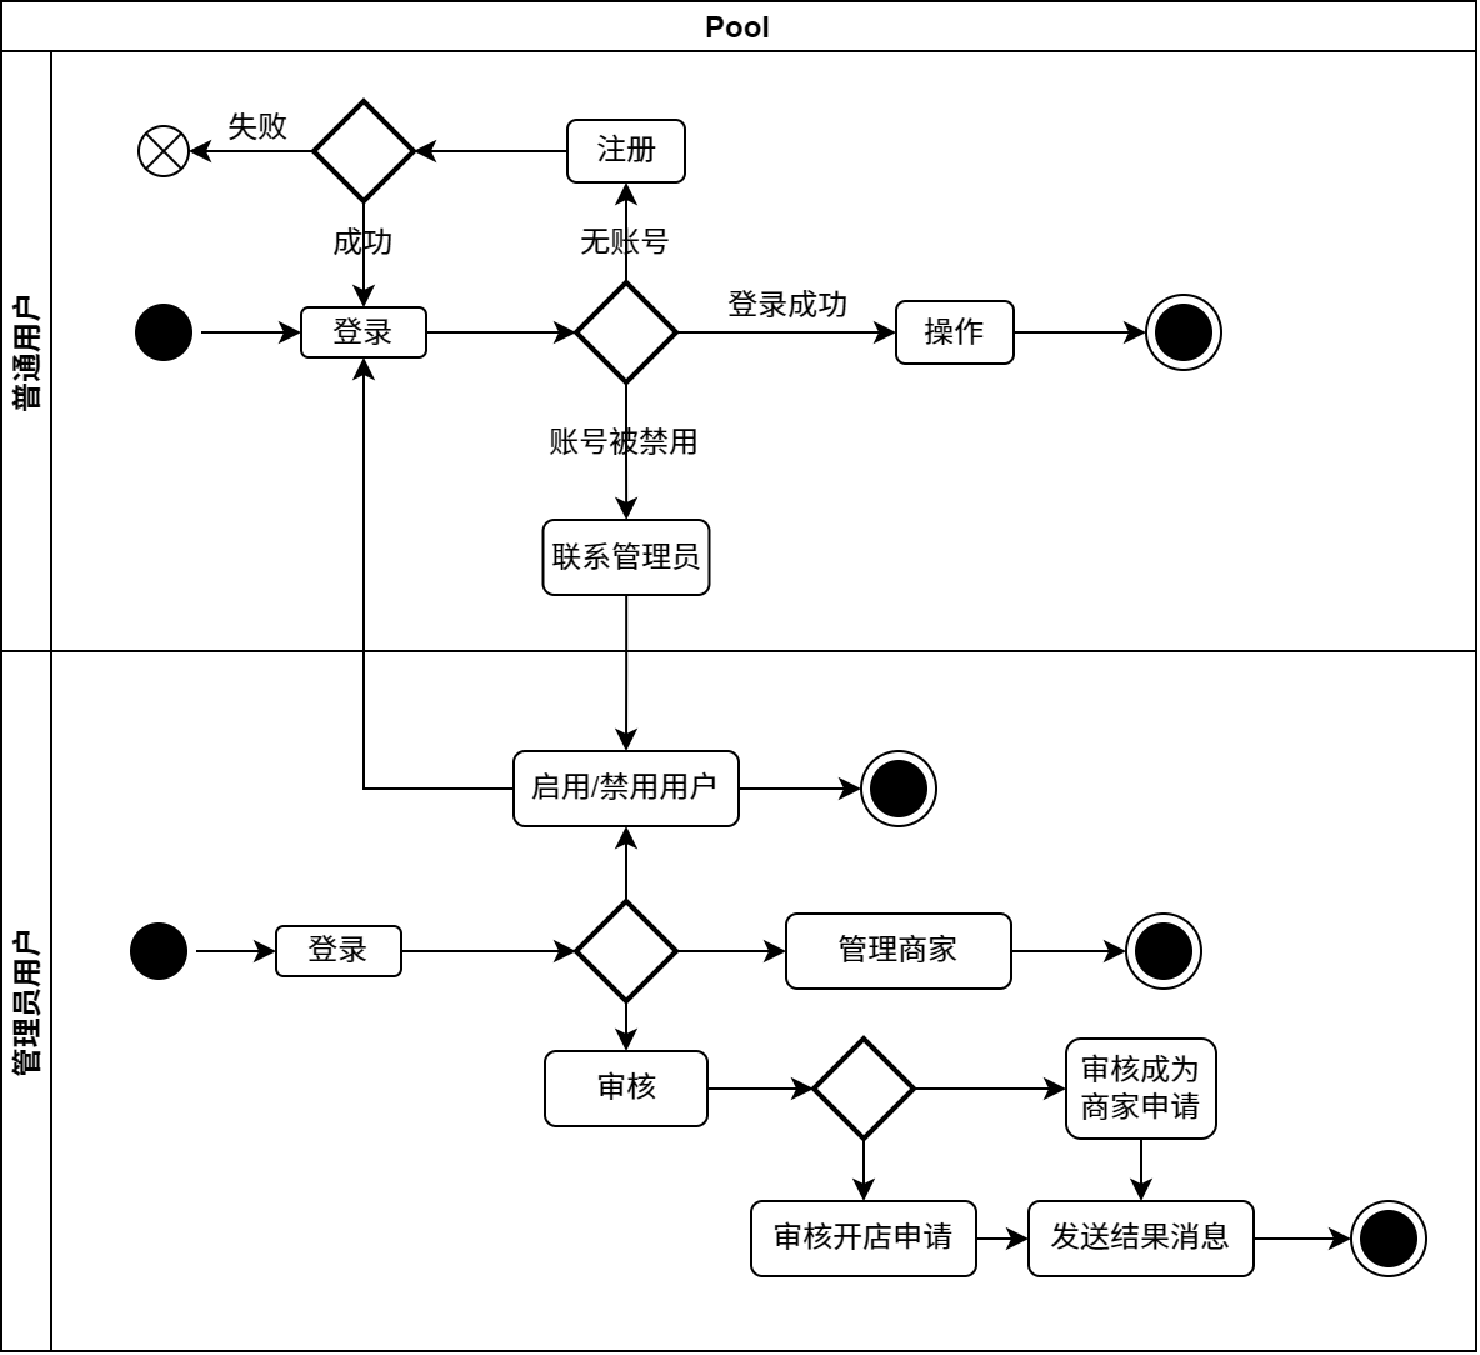
\includegraphics[width=1\textwidth]{figures/in/用户登陆注册活动图}
              \caption{用户登录注册活动图}\label{fig:xml}
              \vspace{\baselineskip}
          \end{figure}


          \newpage

    \item 管理流程

          \begin{figure}[H]
              \centering
              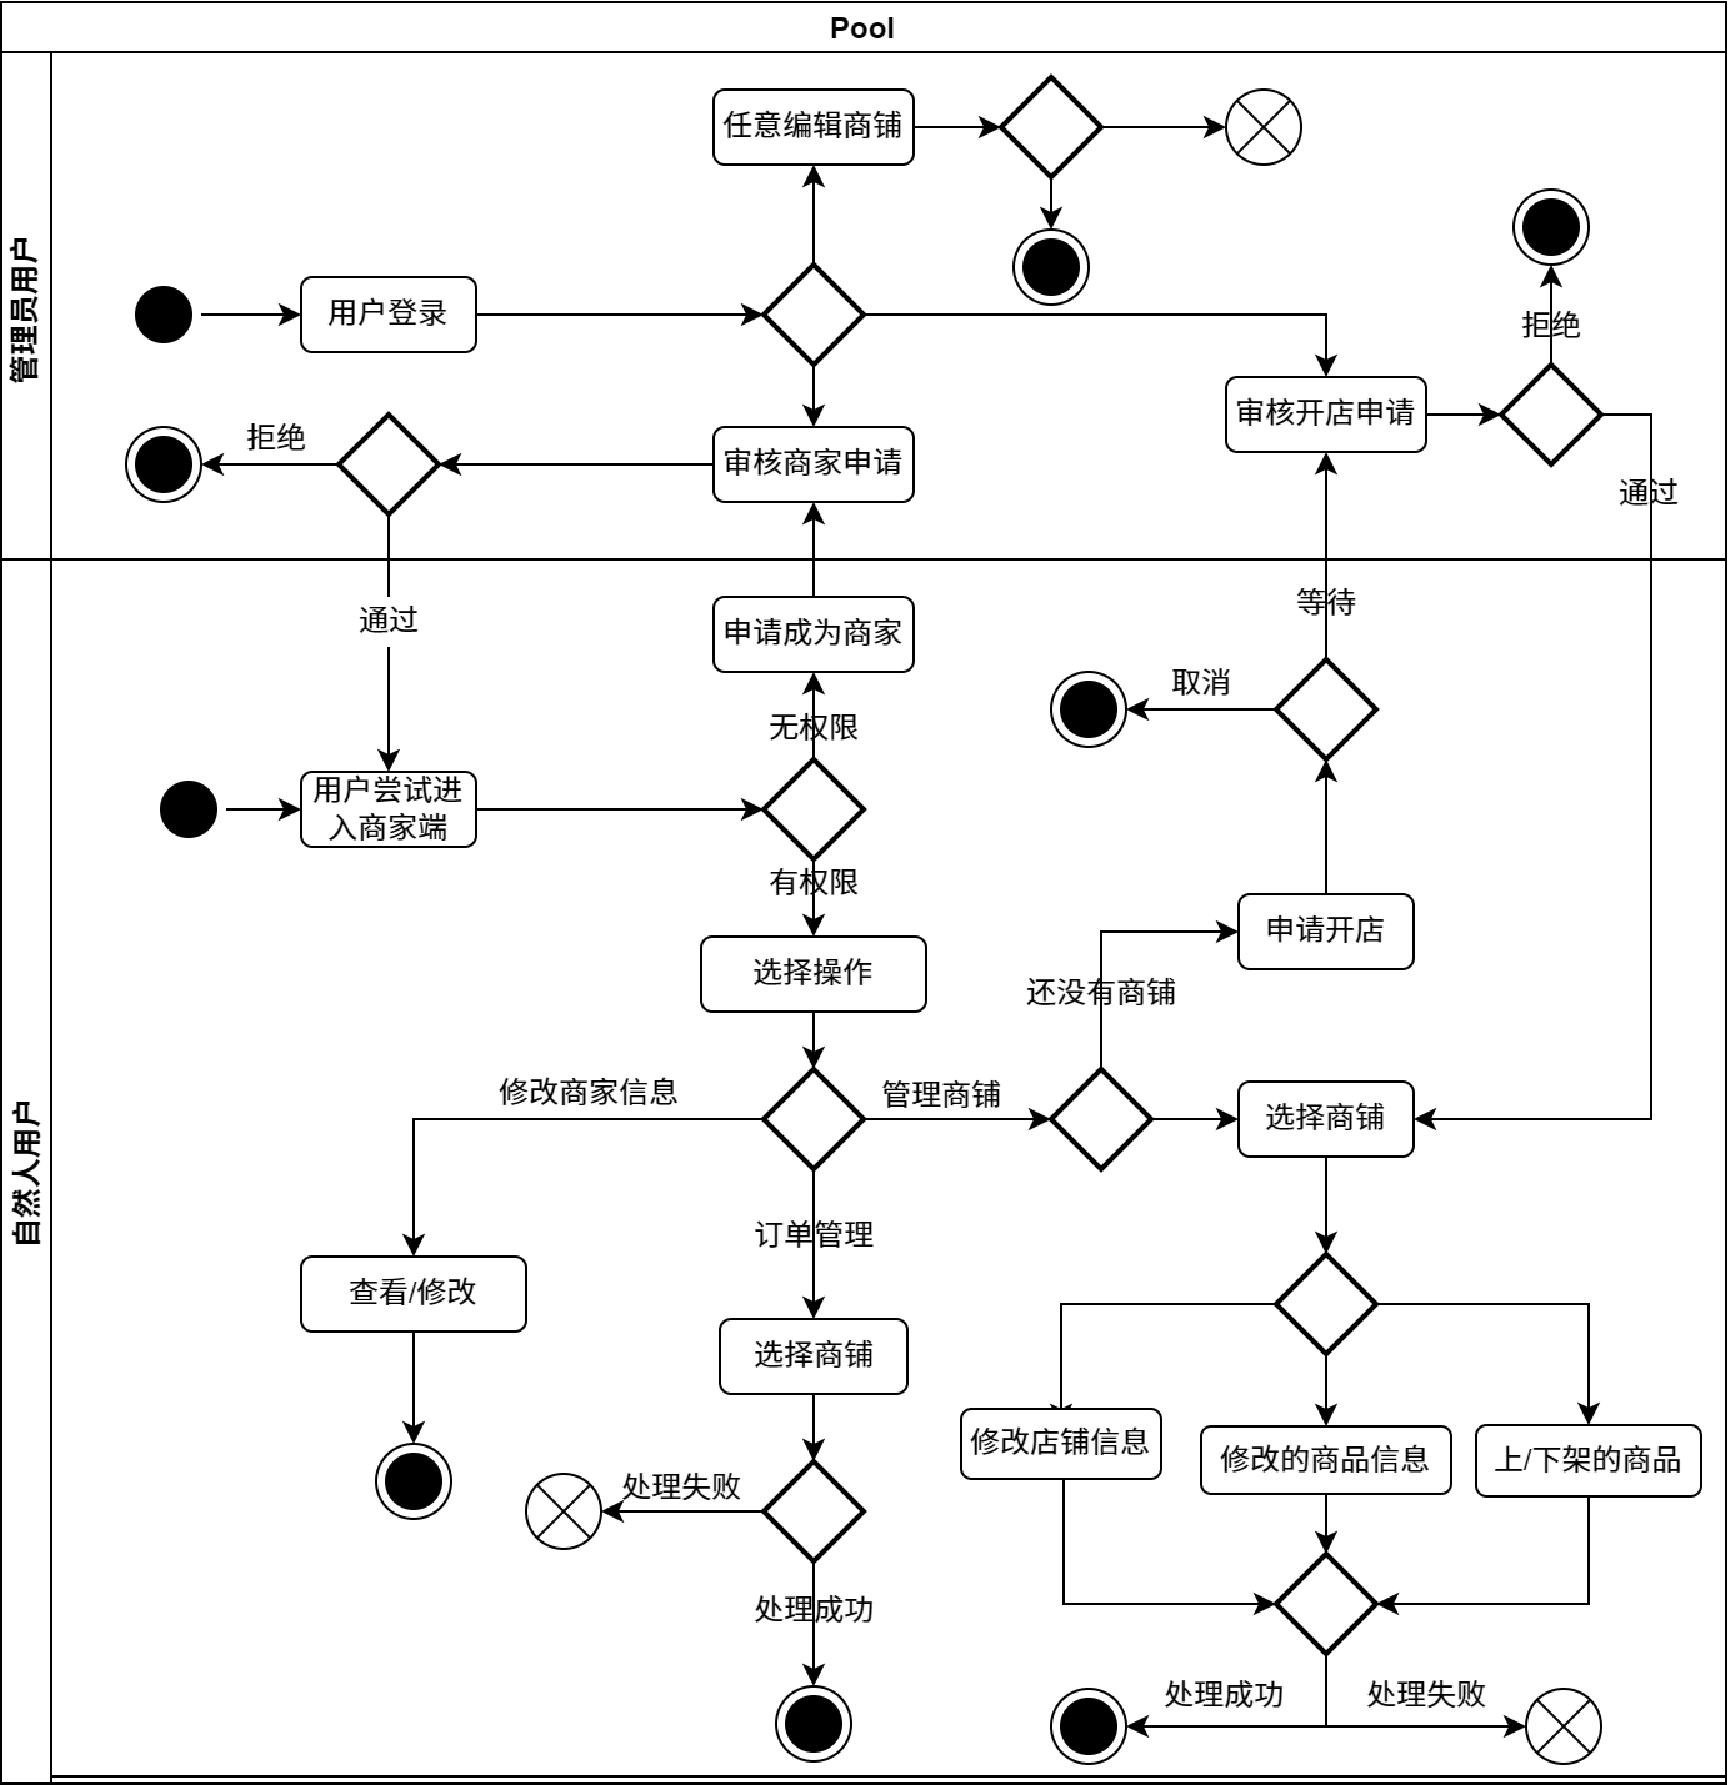
\includegraphics[width=1\textwidth]{figures/in/商家管理活动图}
              \caption{商家管理活动图}\label{fig:xml}
              \vspace{\baselineskip}
          \end{figure}

          \newpage

    \item 订单处理流程

          \begin{figure}[H]
              \centering
              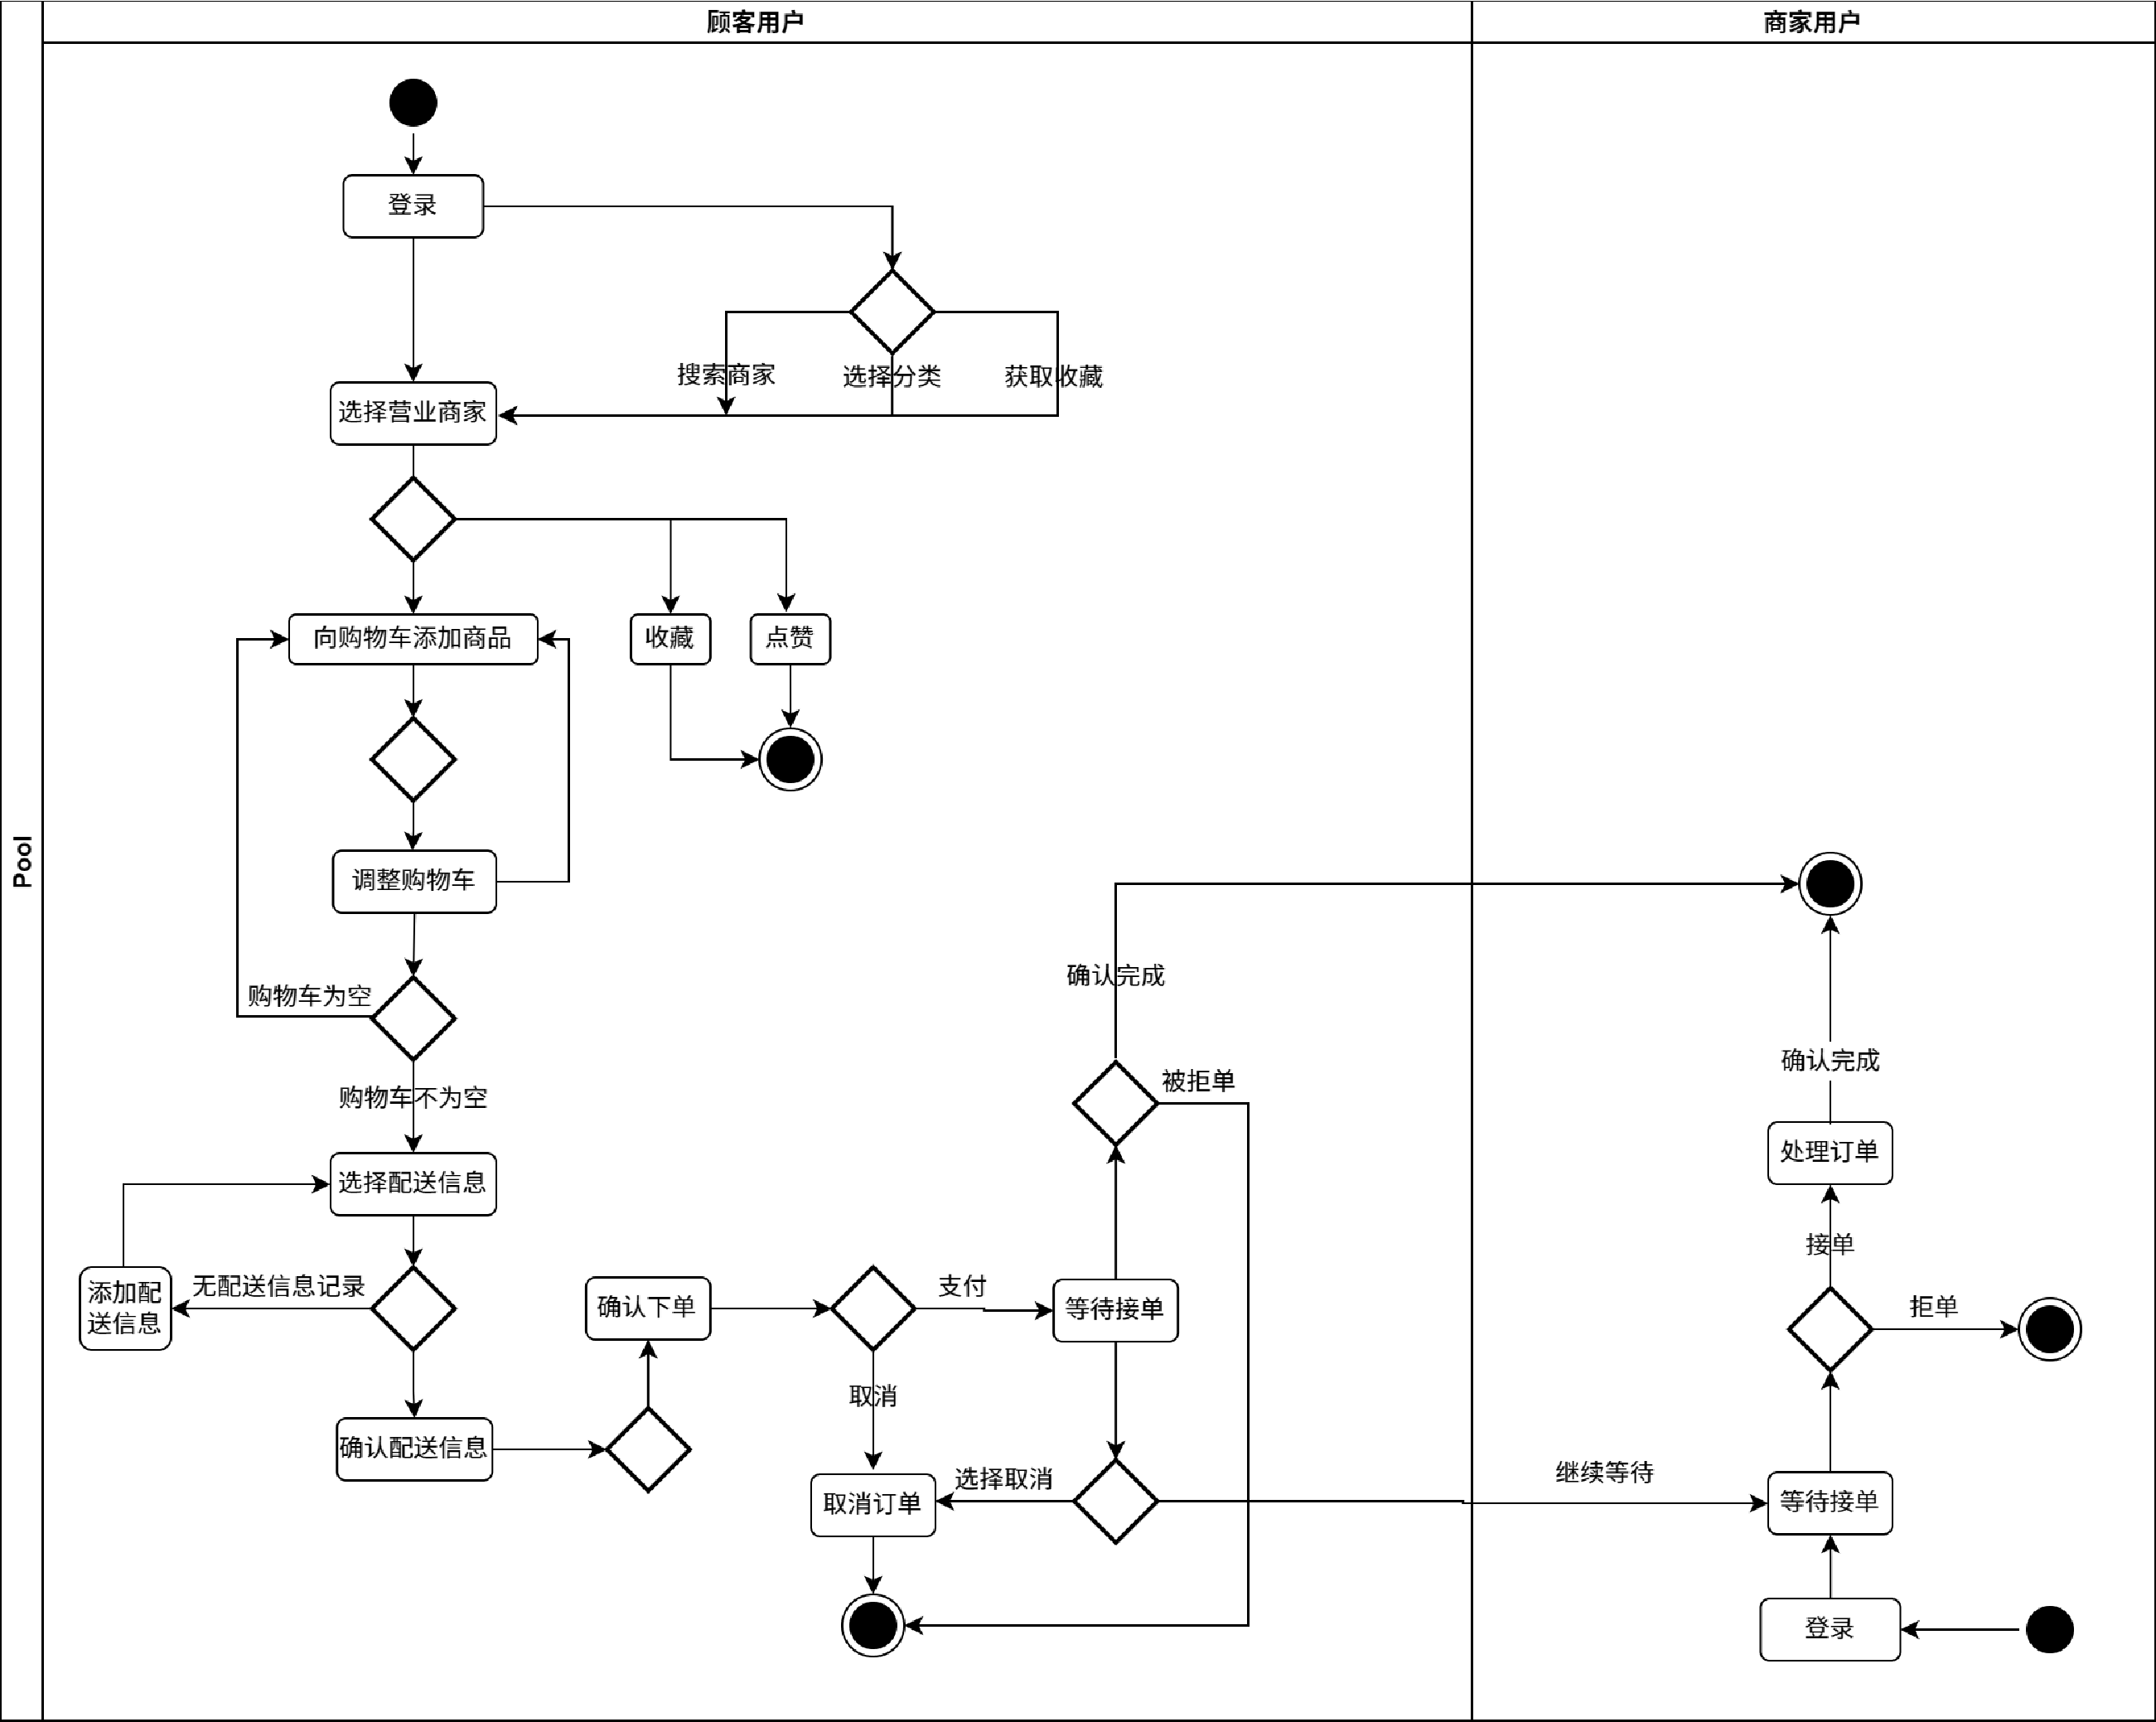
\includegraphics[width=1\textwidth]{figures/in/订单处理活动图}
              \caption{订单处理活动图}\label{fig:xml}
              \vspace{\baselineskip}
          \end{figure}



\end{enumerate}



\section{接口设计}

\subsection{接口统一规范}
为方便响应处理与异常情况的判断，统一将接口响应的数据模型统一为 HttpResult，具体说明如表：
\begin{longtable}{>{\centering\arraybackslash}m{3cm} >{\centering\arraybackslash}m{3cm} >{\centering\arraybackslash}m{4cm}}

    \caption{接口统一规范} \label{tab:training}            \\

    \toprule
    \textbf{字段名 } & \textbf{类型 } & \textbf{说明 }      \\
    \midrule
    \endfirsthead

    \multicolumn{3}{c}{{\tablename\ \thetable{} 续表}} \\
    \toprule
    \textbf{字段名 } & \textbf{类型 } & \textbf{说明 }      \\
    \midrule
    \endhead

    \bottomrule
    \endfoot


    success       & boolean      & 是否出现异常            \\
    code          & string       & 异常状态码             \\
    data          & object       & 返回数据              \\
    message       & string       & 异常信息              \\
\end{longtable}

\subsection{核心接口详情}

\begin{levellist}
    \item \textbf{商铺管理基础接口}
    \begin{levellist}
        \item 根据 ID 修改商铺信息
        \begin{itemize}
            \item 接口路径：PUT /api/businesses/{id}
            \item 路径参数：id（商铺 ID，必填）
            \item 请求体：BusinessUpdateDTO（修改后的商铺信息对象）
            \item 响应：HttpResult<BusinessVO>（修改后的商铺信息对象，包含商家信息）
            \item 关联用户故事 ID：US013（管理商铺信息）
            \item 测试用例：
                  \begin{longtable}{>{\centering\arraybackslash}m{2cm} >{\centering\arraybackslash}m{4cm} >{\centering\arraybackslash}m{5cm} >{\centering\arraybackslash}m{2cm}}

                      \caption{根据 ID 修改商铺信息测试} \label{tab:training}                                           \\

                      \toprule
                      \textbf{用例编号} & \textbf{输入参数（id）}             & \textbf{预期结果}           & \textbf{测试类型} \\
                      \midrule
                      \endfirsthead

                      \multicolumn{4}{c}{{\tablename\ \thetable{} 续表}}                                        \\
                      \toprule
                      \textbf{用例编号} & \textbf{输入参数（id）}             & \textbf{预期结果}           & \textbf{测试类型} \\
                      \midrule
                      \endhead

                      \bottomrule
                      \endfoot

                      TC01          & id=1，name="新商铺名"，address="地址" & code=200，data 返回修改后的商铺  & 正常测试          \\
                      TC02          & id=1，name=""（空字符串）            & code=400，msg="商铺名不能为空"  & 异常测试          \\
                      TC03          & id=9999，name="新名称"            & code=400，msg="商铺不存在"    & 异常测试          \\
                      TC04          & id=1，缺少必填字段                   & code=400，msg="必填字段不能为空" & 异常测试          \\
                  \end{longtable}
        \end{itemize}

        \item 根据 ID 删除商铺
        \begin{itemize}
            \item 接口路径：DELETE /api/businesses/{id}
            \item 路径参数：id（商铺 ID，必填）
            \item 响应：HttpResult<BusinessVO>（删除的商铺信息对象，包含商家信息）
            \item 关联用户故事 ID：US013（管理商铺信息）
            \item 测试用例：
                  \begin{longtable}{>{\centering\arraybackslash}m{2cm} >{\centering\arraybackslash}m{4cm} >{\centering\arraybackslash}m{5cm} >{\centering\arraybackslash}m{2cm}}

                      \caption{根据 ID 删除商铺测试} \label{tab:training}                               \\

                      \toprule
                      \textbf{用例编号} & \textbf{输入参数（id）} & \textbf{预期结果}         & \textbf{测试类型} \\
                      \midrule
                      \endfirsthead

                      \multicolumn{4}{c}{{\tablename\ \thetable{} 续表}}                          \\
                      \toprule
                      \textbf{用例编号} & \textbf{输入参数（id）} & \textbf{预期结果}         & \textbf{测试类型} \\
                      \midrule
                      \endhead

                      \bottomrule
                      \endfoot

                      TC01          & 1                 & code=200，data 返回删除的商铺 & 正常测试          \\
                      TC02          & 9999              & code=400，msg="商铺不存在"  & 异常测试          \\
                      TC03          & 0                 & code=400，msg="参数非法"   & 异常测试          \\
                  \end{longtable}
        \end{itemize}


        \item 修改商铺信息（部分更新）
        \begin{itemize}
            \item 接口路径：PATCH /api/businesses/{id}
            \item 路径参数：id（商铺 ID，必填）
            \item 请求体：BusinessUpdateDTO（修改后的商铺信息对象）
            \item 响应：HttpResult<BusinessVO>（修改后的商铺信息对象）
            \item 关联用户故事 ID：US013（管理商铺信息）
            \item 测试用例：
                  \begin{longtable}{>{\centering\arraybackslash}m{2cm} >{\centering\arraybackslash}m{4cm} >{\centering\arraybackslash}m{5cm} >{\centering\arraybackslash}m{2cm}}

                      \caption{修改商铺信息测试} \label{tab:training}                                     \\

                      \toprule
                      \textbf{用例编号} & \textbf{输入参数（id）} & \textbf{预期结果}           & \textbf{测试类型} \\
                      \midrule
                      \endfirsthead

                      \multicolumn{4}{c}{{\tablename\ \thetable{} 续表}}                            \\
                      \toprule
                      \textbf{用例编号} & \textbf{输入参数（id）} & \textbf{预期结果}           & \textbf{测试类型} \\
                      \midrule
                      \endhead

                      \bottomrule
                      \endfoot

                      TC01          & 部分字段 DTO          & code=200，data 返回修改后的商铺  & 正常测试          \\
                      TC02          & 空 DTO             & code=400，msg="至少需要一个字段" & 异常测试          \\
                  \end{longtable}
        \end{itemize}

        \item 获取所有商铺
        \begin{itemize}
            \item 接口路径：GET /api/businesses
            \item 请求参数：无
            \item 响应：HttpResult<List<BusinessVO>>（商铺数组）
            \item 关联用户故事 ID：US002（浏览商铺列表）
            \item 测试用例：
                  \begin{longtable}{>{\centering\arraybackslash}m{2cm} >{\centering\arraybackslash}m{4cm} >{\centering\arraybackslash}m{5cm} >{\centering\arraybackslash}m{2cm}}

                      \caption{获取所有商铺测试} \label{tab:training}                                  \\

                      \toprule
                      \textbf{用例编号} & \textbf{输入参数（id）} & \textbf{预期结果}        & \textbf{测试类型} \\
                      \midrule
                      \endfirsthead

                      \multicolumn{4}{c}{{\tablename\ \thetable{} 续表}}                         \\
                      \toprule
                      \textbf{用例编号} & \textbf{输入参数（id）} & \textbf{预期结果}        & \textbf{测试类型} \\
                      \midrule
                      \endhead

                      \bottomrule
                      \endfoot

                      TC01          & 无                 & code=200，data 返回所有商铺 & 正常测试          \\
                      TC02          & 无                 & 返回列表不为空              & 正常测试          \\
                  \end{longtable}
        \end{itemize}

        \item 新增商铺
        \begin{itemize}
            \item 接口路径：POST /api/businesses
            \item 请求体：BusinessDTO（新增商家信息对象）
            \item 响应：HttpResult<BusinessVO>（新增的商家对象）
            \item 关联用户故事 ID：US006（申请开店）
            \item 测试用例：
                  \begin{longtable}{>{\centering\arraybackslash}m{2cm} >{\centering\arraybackslash}m{4cm} >{\centering\arraybackslash}m{5cm} >{\centering\arraybackslash}m{2cm}}

                      \caption{新增商铺测试} \label{tab:training}                                       \\

                      \toprule
                      \textbf{用例编号} & \textbf{输入参数（id）} & \textbf{预期结果}           & \textbf{测试类型} \\
                      \midrule
                      \endfirsthead

                      \multicolumn{4}{c}{{\tablename\ \thetable{} 续表}}                            \\
                      \toprule
                      \textbf{用例编号} & \textbf{输入参数（id）} & \textbf{预期结果}           & \textbf{测试类型} \\
                      \midrule
                      \endhead

                      \bottomrule
                      \endfoot

                      TC01          & 有效的 DTO           & code=200，data 返回新增的商铺   & 正常测试          \\
                      TC02          & 缺少必填字段            & code=400，msg="必填字段不能为空" & 异常测试          \\
                  \end{longtable}
        \end{itemize}

        \item 商铺的搜索、筛选与排序
        \begin{itemize}
            \item 接口路径：GET /api/business/search
            \item 请求参数：keyword（搜索关键词）、isScore（是否按评分排序，0/1）、isSales（是否按销售量排序，0/1）
            \item 响应：HttpResult<List<BusinessVO>>（匹配到的商铺信息的数组）
            \item 功能：通过传入的关键字模糊匹配商铺名、商品简介、商铺地址搜索店铺
            \item 关联用户故事 ID：US002（按关键字查询商铺）
            \item 测试用例：
                  \begin{longtable}{>{\centering\arraybackslash}m{2cm} >{\centering\arraybackslash}m{4cm} >{\centering\arraybackslash}m{5cm} >{\centering\arraybackslash}m{2cm}}

                      \caption{商铺的搜索、筛选与排序测试} \label{tab:training}                                                  \\

                      \toprule
                      \textbf{用例编号} & \textbf{输入参数（id）}                    & \textbf{预期结果}          & \textbf{测试类型} \\
                      \midrule
                      \endfirsthead

                      \multicolumn{4}{c}{{\tablename\ \thetable{} 续表}}                                              \\
                      \toprule
                      \textbf{用例编号} & \textbf{输入参数（id）}                    & \textbf{预期结果}          & \textbf{测试类型} \\
                      \midrule
                      \endhead

                      \bottomrule
                      \endfoot

                      TC01          & keyword="火锅"，isScore=0，isSales=0     & code=200，返回火锅相关商铺      & 正常测试          \\
                      TC02          & keyword="xyz123"，isScore=0，isSales=0 & code=200，data 为空列表     & 正常测试          \\
                      TC03          & keyword="商铺"，isScore=1，isSales=0     & code=200，按评分排序         & 正常测试          \\
                      TC04          & keyword="商铺"，isScore=0，isSales=1     & code=200，按销量排序         & 正常测试          \\
                      TC05          & keyword=""（空字符串），isScore=0，isSales=0 & code=400，msg="关键词不能为空" & 异常测试          \\
                      TC06          & keyword="商铺"，isScore=2，isSales=0     & code=400，msg="参数值非法"   & 异常测试          \\
                  \end{longtable}
        \end{itemize}

        \item 商家和管理员新增店铺（带状态）
        \begin{itemize}
            \item 接口路径：POST /api/business/apply
            \item 请求体：business（新增店铺信息）
            \item 响应：HttpResult<Integer>（操作结果）
            \item 权限验证：验证该用户是否有商家或管理员权限
            \item 关联用户故事 ID：US006（申请开店）
            \item 测试用例：
                  \begin{longtable}{>{\centering\arraybackslash}m{2cm} >{\centering\arraybackslash}m{4cm} >{\centering\arraybackslash}m{5cm} >{\centering\arraybackslash}m{2cm}}

                      \caption{商家和管理员新增店铺（带状态）测试} \label{tab:training}                        \\

                      \toprule
                      \textbf{用例编号} & \textbf{输入参数（id）} & \textbf{预期结果}       & \textbf{测试类型} \\
                      \midrule
                      \endfirsthead

                      \multicolumn{4}{c}{{\tablename\ \thetable{} 续表}}                        \\
                      \toprule
                      \textbf{用例编号} & \textbf{输入参数（id）} & \textbf{预期结果}       & \textbf{测试类型} \\
                      \midrule
                      \endhead

                      \bottomrule
                      \endfoot

                      TC01          & 有效的商家信息           & code=200，返回申请 ID    & 正常测试          \\
                      TC02          & 无权限用户             & code=403，msg="权限不足" & 异常测试          \\
                  \end{longtable}
        \end{itemize}

        \item 查询某商家特定状态的所有的店铺
        \begin{itemize}
            \item 接口路径：GET /api/business/merchant
            \item 请求参数：userId（商家 ID）、status（店铺状态：未审核/已审核/审核失败）
            \item 响应：HttpResult<List<BusinessVO>>（所有符合条件的商铺信息数组）
            \item 功能：根据商家 id 查询该商家拥有的所有店铺，同时可以根据传入的 status 字段查询不同状态的商铺
            \item 关联用户故事 ID：US006（查看申请状态）
            \item 测试用例：
                  \begin{longtable}{>{\centering\arraybackslash}m{2cm} >{\centering\arraybackslash}m{4cm} >{\centering\arraybackslash}m{5cm} >{\centering\arraybackslash}m{2cm}}

                      \caption{查询某商家特定状态的所有的店铺测试} \label{tab:training}                           \\

                      \toprule
                      \textbf{用例编号} & \textbf{输入参数（id）}     & \textbf{预期结果}      & \textbf{测试类型} \\
                      \midrule
                      \endfirsthead

                      \multicolumn{4}{c}{{\tablename\ \thetable{} 续表}}                           \\
                      \toprule
                      \textbf{用例编号} & \textbf{输入参数（id）}     & \textbf{预期结果}      & \textbf{测试类型} \\
                      \midrule
                      \endhead

                      \bottomrule
                      \endfoot


                      用例编号          & 输入参数                  & 预期结果               & 测试类型          \\
                      TC01          & userId=1，status="已审核" & code=200，返回已审核的商铺  & 正常测试          \\
                      TC02          & userId=999            & code=200，data 为空列表 & 正常测试          \\
                  \end{longtable}
        \end{itemize}

        \item 查询所有激活的商家
        \begin{itemize}
            \item 接口路径：GET /api/business/active
            \item 请求参数：无
            \item 响应：HttpResult<List<BusinessVO>>（所有符合条件的商家数组）
            \item 功能：管理员查询所有商家集团及其基本信息
            \item 关联用户故事 ID：US013（管理商家集团）
            \item 测试用例：
                  \begin{longtable}{>{\centering\arraybackslash}m{1.7cm} >{\centering\arraybackslash}m{4cm} >{\centering\arraybackslash}m{5.5cm} >{\centering\arraybackslash}m{1.8cm}}

                      \caption{查询所有激活的商家测试} \label{tab:training}                           \\

                      \toprule
                      \textbf{用例编号} & \textbf{输入参数（id）} & \textbf{预期结果}    & \textbf{测试类型} \\
                      \midrule
                      \endfirsthead

                      \multicolumn{4}{c}{{\tablename\ \thetable{} 续表}}                     \\
                      \toprule
                      \textbf{用例编号} & \textbf{输入参数（id）} & \textbf{预期结果}    & \textbf{测试类型} \\
                      \midrule
                      \endhead

                      \bottomrule
                      \endfoot

                      TC01          & 无                 & code=200，返回激活的商家 & 正常测试          \\
                  \end{longtable}
        \end{itemize}

        \item 查询不同类型的店铺
        \begin{itemize}
            \item 接口路径：GET /api/business/type
            \item 请求参数：type（查询的类型 id，范围 1~10）
            \item 响应：HttpResult<List<BusinessVO>>
            \item 功能：查询十种类型的商铺
            \item 关联用户故事 ID：US002（按品类查询商铺）
            \item 测试用例：
                  \begin{longtable}{>{\centering\arraybackslash}m{1.7cm} >{\centering\arraybackslash}m{4cm} >{\centering\arraybackslash}m{5.5cm} >{\centering\arraybackslash}m{1.8cm}}

                      \caption{查询不同类型的店铺测试} \label{tab:training}                               \\

                      \toprule
                      \textbf{用例编号} & \textbf{输入参数（id）} & \textbf{预期结果}        & \textbf{测试类型} \\
                      \midrule
                      \endfirsthead

                      \multicolumn{4}{c}{{\tablename\ \thetable{} 续表}}                         \\
                      \toprule
                      \textbf{用例编号} & \textbf{输入参数（id）} & \textbf{预期结果}        & \textbf{测试类型} \\
                      \midrule
                      \endhead

                      \bottomrule
                      \endfoot

                      TC01          & type=1            & code=200，返回该类型商铺     & 正常测试          \\
                      TC02          & type=11           & code=400，msg="类型不存在" & 异常测试          \\
                  \end{longtable}
        \end{itemize}

        \item 查询轮播图商铺
        \begin{itemize}
            \item 接口路径：GET /api/business/carousel
            \item 请求参数：无
            \item 响应：HttpResult<List<BusinessSearchVO>>（销量前三的商铺及其基本信息）
            \item 功能：返回销量前三的商铺及其基本信息
            \item 关联用户故事 ID：US002（首页轮播展示）
            \item 测试用例：
                  \begin{longtable}{>{\centering\arraybackslash}m{2cm} >{\centering\arraybackslash}m{4cm} >{\centering\arraybackslash}m{5cm} >{\centering\arraybackslash}m{2cm}}

                      \caption{查询轮播图商铺测试} \label{tab:training}                            \\

                      \toprule
                      \textbf{用例编号} & \textbf{输入参数（id）} & \textbf{预期结果}   & \textbf{测试类型} \\
                      \midrule
                      \endfirsthead

                      \multicolumn{4}{c}{{\tablename\ \thetable{} 续表}}                    \\
                      \toprule
                      \textbf{用例编号} & \textbf{输入参数（id）} & \textbf{预期结果}   & \textbf{测试类型} \\
                      \midrule
                      \endhead

                      \bottomrule
                      \endfoot


                      TC01          & 无                 & code=200，返回前三商铺 & 正常测试          \\
                  \end{longtable}
        \end{itemize}

        \item 更新某店铺信息（带状态）
        \begin{itemize}
            \item 接口路径：PUT /api/business/own
            \item 请求参数：id（店铺 ID）
            \item 请求体：BusinessUpdateDTO（店铺更新信息）
            \item 响应：HttpResult<BusinessVO>
            \item 关联用户故事 ID：US008（商家管理店铺）
            \item 测试用例：
                  \begin{longtable}{>{\centering\arraybackslash}m{2cm} >{\centering\arraybackslash}m{4cm} >{\centering\arraybackslash}m{5cm} >{\centering\arraybackslash}m{2cm}}

                      \caption{更新某店铺信息（带状态）测试} \label{tab:training}                              \\

                      \toprule
                      \textbf{用例编号} & \textbf{输入参数（id）} & \textbf{预期结果}          & \textbf{测试类型} \\
                      \midrule
                      \endfirsthead

                      \multicolumn{4}{c}{{\tablename\ \thetable{} 续表}}                           \\
                      \toprule
                      \textbf{用例编号} & \textbf{输入参数（id）} & \textbf{预期结果}          & \textbf{测试类型} \\
                      \midrule
                      \endhead

                      \bottomrule
                      \endfoot

                      TC01          & 有效的 DTO           & code=200，data 返回修改后的商铺 & 正常测试          \\
                  \end{longtable}
        \end{itemize}

    \end{levellist}

    \item \textbf{用户模块接口定义}
    \begin{levellist}

        \item 新增用户（仅登录账号）
        \begin{itemize}
            \item 接口路径：POST /api/users
            \item 请求体：UserCreateDTO（请求体包含用户创建信息）
            \item 响应：HttpResult<UserVO>（返回创建的用户信息）
            \item 关联用户故事 ID：US001（用户注册）
            \item 测试用例：
                  \begin{longtable}{>{\centering\arraybackslash}m{2cm} >{\centering\arraybackslash}m{4cm} >{\centering\arraybackslash}m{5cm} >{\centering\arraybackslash}m{2cm}}

                      \caption{新增用户（仅登录账号）测试} \label{tab:training}                              \\

                      \toprule
                      \textbf{用例编号} & \textbf{输入参数（id）} & \textbf{预期结果}         & \textbf{测试类型} \\
                      \midrule
                      \endfirsthead

                      \multicolumn{4}{c}{{\tablename\ \thetable{} 续表}}                          \\
                      \toprule
                      \textbf{用例编号} & \textbf{输入参数（id）} & \textbf{预期结果}         & \textbf{测试类型} \\
                      \midrule
                      \endhead

                      \bottomrule
                      \endfoot

                      TC01          & 有效的用户信息           & code=200，返回用户信息       & 正常测试          \\
                      TC02          & 用户名已存在            & code=400，msg="用户名已存在" & 异常测试          \\
                  \end{longtable}
        \end{itemize}

        \item 顾客注册
        \begin{itemize}
            \item 接口路径：POST /api/register
            \item 请求体：PersonCreateDTO（请求体包含自然人用户创建信息）
            \item 响应：HttpResult<PersonVO>（返回创建的自然人用户信息）
            \item 关联用户故事 ID：US001（用户注册）
            \item 测试用例：
                  \begin{longtable}{>{\centering\arraybackslash}m{2cm} >{\centering\arraybackslash}m{5cm} >{\centering\arraybackslash}m{4cm} >{\centering\arraybackslash}m{2cm}}

                      \caption{顾客注册测试} \label{tab:training}                                                                                                                 \\

                      \toprule
                      \textbf{用例编号} & \textbf{输入参数（id）}                                                                     & \textbf{预期结果}                 & \textbf{测试类型} \\
                      \midrule
                      \endfirsthead

                      \multicolumn{4}{c}{{\tablename\ \thetable{} 续表}}                                                                                                      \\
                      \toprule
                      \textbf{用例编号} & \textbf{输入参数（id）}                                                                     & \textbf{预期结果}                 & \textbf{测试类型} \\
                      \midrule
                      \endhead

                      \bottomrule
                      \endfoot

                      TC01          & username="newuser"，password="Abc123456"，email="user@example.com"，phone="13800138000"  & code=200，返回用户信息               & 正常测试          \\
                      TC02          & username="newuser"，password="123456"，email="user@example.com"，phone="13800138000"     & code=400，msg="密码必须包含大小写字母和数字" & 异常测试          \\
                      TC03          & username="newuser"，password="Abc123456"，email="invalid-email"，phone="13800138000"     & code=400，msg="邮箱格式错误"         & 异常测试          \\
                      TC04          & username="newuser"，password="Abc123456"，email="user@example.com"，phone="138001380"    & code=400，msg="手机号格式错误"        & 异常测试          \\
                      TC05          & username="testuser"，password="Abc123456"，email="user@example.com"，phone="13800138000" & code=400，msg="用户名已存在"         & 异常测试          \\
                      TC06          & username=""，password="Abc123456"，email="user@example.com"，phone="13800138000"         & code=400，msg="用户名不能为空"        & 异常测试          \\
                  \end{longtable}
        \end{itemize}

        \item 新增自然人用户
        \begin{itemize}
            \item 接口路径：POST /api/persons
            \item 请求体：PersonCreateDTO（请求体包含自然人用户创建信息）
            \item 响应：HttpResult<PersonVO>（返回创建的自然人用户信息）
            \item 关联用户故事 ID：US001（用户注册）
            \item 测试用例：
                  \begin{longtable}{>{\centering\arraybackslash}m{2cm} >{\centering\arraybackslash}m{4cm} >{\centering\arraybackslash}m{5cm} >{\centering\arraybackslash}m{2cm}}

                      \caption{新增自然人用户测试} \label{tab:training}                            \\

                      \toprule
                      \textbf{用例编号} & \textbf{输入参数（id）} & \textbf{预期结果}   & \textbf{测试类型} \\
                      \midrule
                      \endfirsthead

                      \multicolumn{4}{c}{{\tablename\ \thetable{} 续表}}                    \\
                      \toprule
                      \textbf{用例编号} & \textbf{输入参数（id）} & \textbf{预期结果}   & \textbf{测试类型} \\
                      \midrule
                      \endhead

                      \bottomrule
                      \endfoot

                      TC01          & 有效的用户信息           & code=200，返回用户信息 & 正常测试          \\
                  \end{longtable}
        \end{itemize}


        \item 修改密码
        \begin{itemize}
            \item 接口路径：POST /api/password
            \item 请求体：LoginDTO（请求体包含用户名和密码）
            \item 响应：HttpResult<String>（返回操作结果）
            \item 关联用户故事 ID：US001（用户账号管理）
            \item 测试用例：
                  \begin{longtable}{>{\centering\arraybackslash}m{1.7cm} >{\centering\arraybackslash}m{4cm} >{\centering\arraybackslash}m{5.5cm} >{\centering\arraybackslash}m{1.8cm}}

                      \caption{修改密码测试} \label{tab:training}                                   \\

                      \toprule
                      \textbf{用例编号} & \textbf{输入参数（id）} & \textbf{预期结果}       & \textbf{测试类型} \\
                      \midrule
                      \endfirsthead

                      \multicolumn{4}{c}{{\tablename\ \thetable{} 续表}}                        \\
                      \toprule
                      \textbf{用例编号} & \textbf{输入参数（id）} & \textbf{预期结果}       & \textbf{测试类型} \\
                      \midrule
                      \endhead

                      \bottomrule
                      \endfoot

                      TC01          & 正确的旧密码            & code=200，msg="修改成功" & 正常测试          \\
                      TC02          & 错误的旧密码            & code=400，msg="密码错误" & 异常测试          \\
                  \end{longtable}
        \end{itemize}

        \item 获取当前登录用户
        \begin{itemize}
            \item 接口路径：GET /api/user
            \item 请求参数：无
            \item 响应：HttpResult<UserVO>（返回当前登录用户信息）
            \item 关联用户故事 ID：US001（用户登录）
            \item 测试用例：
                  \begin{longtable}{>{\centering\arraybackslash}m{2cm} >{\centering\arraybackslash}m{4cm} >{\centering\arraybackslash}m{5cm} >{\centering\arraybackslash}m{2cm}}

                      \caption{获取当前登录用户测试} \label{tab:training}                              \\

                      \toprule
                      \textbf{用例编号} & \textbf{输入参数（id）} & \textbf{预期结果}      & \textbf{测试类型} \\
                      \midrule
                      \endfirsthead

                      \multicolumn{4}{c}{{\tablename\ \thetable{} 续表}}                       \\
                      \toprule
                      \textbf{用例编号} & \textbf{输入参数（id）} & \textbf{预期结果}      & \textbf{测试类型} \\
                      \midrule
                      \endhead

                      \bottomrule
                      \endfoot


                      TC01          & 有效的 token         & code=200，返回用户信息    & 正常测试          \\
                      TC02          & 无 token           & code=401，msg="未授权" & 异常测试          \\
                  \end{longtable}
        \end{itemize}

        \item 用户登录认证
        \begin{itemize}
            \item 接口路径：POST /api/auth
            \item 请求体：LoginDTO（请求体包含登录凭证）
            \item 响应：HttpResult<JWTToken>（返回认证令牌）
            \item 关联用户故事 ID：US001（用户登录）
            \item 测试用例：
                  \begin{longtable}{>{\centering\arraybackslash}m{2cm} >{\centering\arraybackslash}m{4cm} >{\centering\arraybackslash}m{5cm} >{\centering\arraybackslash}m{2cm}}

                      \caption{用户登录认证测试} \label{tab:training}                                                                \\

                      \toprule
                      \textbf{用例编号} & \textbf{输入参数（id）}                           & \textbf{预期结果}            & \textbf{测试类型} \\
                      \midrule
                      \endfirsthead

                      \multicolumn{4}{c}{{\tablename\ \thetable{} 续表}}                                                       \\
                      \toprule
                      \textbf{用例编号} & \textbf{输入参数（id）}                           & \textbf{预期结果}            & \textbf{测试类型} \\
                      \midrule
                      \endhead

                      \bottomrule
                      \endfoot

                      TC01          & username="testuser"，password="Abc123456"    & code=200，返回 JWT token    & 正常测试          \\
                      TC02          & username="testuser"，password="wrongpass"    & code=400，msg="用户名或密码错误"  & 异常测试          \\
                      TC03          & username="nonexistent"，password="Abc123456" & code=400，msg="用户名或密码错误"  & 异常测试          \\
                      TC04          & username=""，password="Abc123456"            & code=400，msg="用户名不能为空"   & 异常测试          \\
                      TC05          & username="testuser"，password=""             & code=400，msg="密码不能为空"    & 异常测试          \\
                      TC06          & username="testuser"，password="123"          & code=400，msg="密码长度不符合要求" & 异常测试          \\
                  \end{longtable}
        \end{itemize}

        \item 启用/禁用用户
        \begin{itemize}
            \item 接口路径：PUT /api/{username}/status
            \item 路径参数：username（用户名，必填）
            \item 请求参数：activated（查询参数表示是否激活）
            \item 响应：HttpResult<String>（返回操作结果消息）
            \item 关联用户故事 ID：US012（管理员管理用户）
            \item 测试用例：
                  \begin{longtable}{>{\centering\arraybackslash}m{1.7cm} >{\centering\arraybackslash}m{3.7cm} >{\centering\arraybackslash}m{6cm} >{\centering\arraybackslash}m{1.7cm}}

                      \caption{启用/禁用用户测试} \label{tab:training}                                 \\

                      \toprule
                      \textbf{用例编号} & \textbf{输入参数（id）} & \textbf{预期结果}        & \textbf{测试类型} \\
                      \midrule
                      \endfirsthead

                      \multicolumn{4}{c}{{\tablename\ \thetable{} 续表}}                         \\
                      \toprule
                      \textbf{用例编号} & \textbf{输入参数（id）} & \textbf{预期结果}        & \textbf{测试类型} \\
                      \midrule
                      \endhead

                      \bottomrule
                      \endfoot

                      TC01          & activated=1       & code=200，msg="启用成功"  & 正常测试          \\
                      TC02          & activated=0       & code=200，msg="禁用成功"  & 正常测试          \\
                      TC03          & 不存在的用户            & code=400，msg="用户不存在" & 异常测试          \\
                  \end{longtable}
        \end{itemize}

        \item 切换用户启用/禁用状态
        \begin{itemize}
            \item 接口路径：PATCH /api/{username}/status
            \item 路径参数：username（用户名，必填）
            \item 响应：HttpResult<UserVO>（返回用户信息）
            \item 关联用户故事 ID：US012（管理员管理用户）
            \item 测试用例：
                  \begin{longtable}{>{\centering\arraybackslash}m{2cm} >{\centering\arraybackslash}m{4cm} >{\centering\arraybackslash}m{5cm} >{\centering\arraybackslash}m{2cm}}

                      \caption{切换用户启用/禁用状态测试} \label{tab:training}                        \\

                      \toprule
                      \textbf{用例编号} & \textbf{输入参数（id）} & \textbf{预期结果}   & \textbf{测试类型} \\
                      \midrule
                      \endfirsthead

                      \multicolumn{4}{c}{{\tablename\ \thetable{} 续表}}                    \\
                      \toprule
                      \textbf{用例编号} & \textbf{输入参数（id）} & \textbf{预期结果}   & \textbf{测试类型} \\
                      \midrule
                      \endhead

                      \bottomrule
                      \endfoot

                      TC01          & 启用的用户             & code=200，状态变为禁用 & 正常测试          \\
                      TC02          & 禁用的用户             & code=200，状态变为启用 & 正常测试          \\
                  \end{longtable}
        \end{itemize}

        \item 修改个人信息
        \begin{itemize}
            \item 接口路径：PUT /api/person/info
            \item 请求体：PersonUpdateDTO（请求体包含个人信息更新内容）
            \item 响应：HttpResult<Person>（返回完整的个人信息）
            \item 关联用户故事 ID：US001（用户账号管理）
            \item 测试用例：
                  \begin{longtable}{>{\centering\arraybackslash}m{1.7cm} >{\centering\arraybackslash}m{4cm} >{\centering\arraybackslash}m{5.5cm} >{\centering\arraybackslash}m{1.8cm}}

                      \caption{修改个人信息测试} \label{tab:training}                                   \\

                      \toprule
                      \textbf{用例编号} & \textbf{输入参数（id）} & \textbf{预期结果}         & \textbf{测试类型} \\
                      \midrule
                      \endfirsthead

                      \multicolumn{4}{c}{{\tablename\ \thetable{} 续表}}                          \\
                      \toprule
                      \textbf{用例编号} & \textbf{输入参数（id）} & \textbf{预期结果}         & \textbf{测试类型} \\
                      \midrule
                      \endhead

                      \bottomrule
                      \endfoot

                      TC01          & 有效的更新信息           & code=200，返回更新后的信息     & 正常测试          \\
                      TC02          & 邮箱格式错误            & code=400，msg="邮箱格式错误" & 异常测试          \\
                  \end{longtable}
        \end{itemize}

        \item 获取不同状态的自然人用户
        \begin{itemize}
            \item 接口路径：GET /api/persons
            \item 请求参数：status（查询参数表示用户状态）
            \item 响应：HttpResult<List<PersonVO>>（返回自然人用户列表）
            \item 关联用户故事 ID：US012（管理员管理用户）
            \item 测试用例：
                  \begin{longtable}{>{\centering\arraybackslash}m{1.7cm} >{\centering\arraybackslash}m{4cm} >{\centering\arraybackslash}m{5.3cm} >{\centering\arraybackslash}m{2cm}}

                      \caption{获取不同状态的自然人用户测试} \label{tab:training}                        \\

                      \toprule
                      \textbf{用例编号} & \textbf{输入参数（id）} & \textbf{预期结果}    & \textbf{测试类型} \\
                      \midrule
                      \endfirsthead

                      \multicolumn{4}{c}{{\tablename\ \thetable{} 续表}}                     \\
                      \toprule
                      \textbf{用例编号} & \textbf{输入参数（id）} & \textbf{预期结果}    & \textbf{测试类型} \\
                      \midrule
                      \endhead

                      \bottomrule
                      \endfoot

                      TC01          & status="启用"       & code=200，返回启用的用户 & 正常测试          \\
                      TC02          & status="禁用"       & code=200，返回禁用的用户 & 正常测试          \\
                  \end{longtable}
        \end{itemize}

        \item 搜索用户
        \begin{itemize}
            \item 接口路径：POST /api/persons/search
            \item 请求体：UserSearchDTO（请求体包含搜索关键词和状态）
            \item 响应：HttpResult<List<PersonVO>>（返回搜索到的用户列表）
            \item 关联用户故事 ID：US012（管理员管理用户）
            \item 测试用例：
                  \begin{longtable}{>{\centering\arraybackslash}m{1.7cm} >{\centering\arraybackslash}m{4cm} >{\centering\arraybackslash}m{5.3cm} >{\centering\arraybackslash}m{2cm}}

                      \caption{搜索用户测试} \label{tab:training}                                  \\

                      \toprule
                      \textbf{用例编号} & \textbf{输入参数（id）} & \textbf{预期结果}      & \textbf{测试类型} \\
                      \midrule
                      \endfirsthead

                      \multicolumn{4}{c}{{\tablename\ \thetable{} 续表}}                       \\
                      \toprule
                      \textbf{用例编号} & \textbf{输入参数（id）} & \textbf{预期结果}      & \textbf{测试类型} \\
                      \midrule
                      \endhead

                      \bottomrule
                      \endfoot

                      TC01          & keyword="张"       & code=200，返回匹配的用户   & 正常测试          \\
                      TC02          & keyword="不存在"     & code=200，data 为空列表 & 正常测试          \\
                  \end{longtable}
        \end{itemize}

        \item 根据 ID 获取自然人属性
        \begin{itemize}
            \item 接口路径：GET /api/personInfo
            \item 请求参数：id（查询参数表示用户 ID）
            \item 响应：HttpResult<Person>（返回指定用户的完整个人信息）
            \item 关联用户故事 ID：US001（用户账号管理）
            \item 测试用例：
                  \begin{longtable}{>{\centering\arraybackslash}m{1.7cm} >{\centering\arraybackslash}m{3.3cm} >{\centering\arraybackslash}m{6cm} >{\centering\arraybackslash}m{2cm}}

                      \caption{根据 ID 获取自然人属性测试} \label{tab:training}                           \\

                      \toprule
                      \textbf{用例编号} & \textbf{输入参数（id）} & \textbf{预期结果}        & \textbf{测试类型} \\
                      \midrule
                      \endfirsthead

                      \multicolumn{4}{c}{{\tablename\ \thetable{} 续表}}                         \\
                      \toprule
                      \textbf{用例编号} & \textbf{输入参数（id）} & \textbf{预期结果}        & \textbf{测试类型} \\
                      \midrule
                      \endhead

                      \bottomrule
                      \endfoot

                      TC01          & id=1              & code=200，返回用户信息      & 正常测试          \\
                      TC02          & id=999            & code=400，msg="用户不存在" & 异常测试          \\
                  \end{longtable}
        \end{itemize}

        \item 删除用户
        \begin{itemize}
            \item 接口路径：DELETE /api/{username}
            \item 路径参数：username（用户名，必填）
            \item 响应：HttpResult（返回操作结果）
            \item 关联用户故事 ID：US012（管理员管理用户）
            \item 测试用例：
                  \begin{longtable}{>{\centering\arraybackslash}m{1.7cm} >{\centering\arraybackslash}m{3.3cm} >{\centering\arraybackslash}m{6cm} >{\centering\arraybackslash}m{2cm}}

                      \caption{删除用户测试} \label{tab:training}                                    \\

                      \toprule
                      \textbf{用例编号} & \textbf{输入参数（id）} & \textbf{预期结果}        & \textbf{测试类型} \\
                      \midrule
                      \endfirsthead

                      \multicolumn{4}{c}{{\tablename\ \thetable{} 续表}}                         \\
                      \toprule
                      \textbf{用例编号} & \textbf{输入参数（id）} & \textbf{预期结果}        & \textbf{测试类型} \\
                      \midrule
                      \endhead

                      \bottomrule
                      \endfoot

                      TC01          & 存在的用户             & code=200，msg="删除成功"  & 正常测试          \\
                      TC02          & 不存在的用户            & code=400，msg="用户不存在" & 异常测试          \\
                  \end{longtable}
        \end{itemize}

    \end{levellist}

    \item \textbf{地址与权限模块接口定义}
    \begin{levellist}
        \item 新增地址
        \begin{itemize}
            \item 接口路径：POST /api/addresses
            \item 请求体：AddressCreateDTO（请求体包含地址创建信息）
            \item 响应：HttpResult<AddressVO>（返回创建的地址信息）
            \item 关联用户故事 ID：US004（管理收货地址）
            \item 测试用例：
                  \begin{longtable}{>{\centering\arraybackslash}m{1.7cm} >{\centering\arraybackslash}m{6cm} >{\centering\arraybackslash}m{3.5cm} >{\centering\arraybackslash}m{1.8cm}}

                      \caption{新增地址测试} \label{tab:training}                                                                             \\

                      \toprule
                      \textbf{用例编号} & \textbf{输入参数（id）}                                        & \textbf{预期结果}          & \textbf{测试类型} \\
                      \midrule
                      \endfirsthead

                      \multicolumn{4}{c}{{\tablename\ \thetable{} 续表}}                                                                  \\
                      \toprule
                      \textbf{用例编号} & \textbf{输入参数（id）}                                        & \textbf{预期结果}          & \textbf{测试类型} \\
                      \midrule
                      \endhead

                      \bottomrule
                      \endfoot

                      TC01          & contactName="张三"，phone="13800138000"，address="北京市朝阳区某街道" & code=200，返回地址信息        & 正常测试          \\
                      TC02          & contactName="张三"，phone="12345678901"，address="北京市朝阳区某街道" & code=400，msg="手机号格式错误" & 异常测试          \\
                      TC03          & contactName=""，phone="13800138000"，address="北京市朝阳区某街道"   & code=400，msg="联系人不能为空" & 异常测试          \\
                      TC04          & contactName="张三"，phone="13800138000"，address=""          & code=400，msg="地址不能为空"  & 异常测试          \\
                  \end{longtable}
        \end{itemize}


        \item 删除配送地址
        \begin{itemize}
            \item 接口路径：POST /api/addresses/removeDeliveryAddress
            \item 请求体：DeliveryAddress（请求体包含地址信息）
            \item 响应：HttpResult（返回操作结果）
            \item 关联用户故事 ID：US004（管理收货地址）
            \item 测试用例：
                  \begin{longtable}{>{\centering\arraybackslash}m{1.7cm} >{\centering\arraybackslash}m{3cm} >{\centering\arraybackslash}m{6.3cm} >{\centering\arraybackslash}m{2cm}}

                      \caption{删除配送地址测试} \label{tab:training}                                  \\

                      \toprule
                      \textbf{用例编号} & \textbf{输入参数（id）} & \textbf{预期结果}        & \textbf{测试类型} \\
                      \midrule
                      \endfirsthead

                      \multicolumn{4}{c}{{\tablename\ \thetable{} 续表}}                         \\
                      \toprule
                      \textbf{用例编号} & \textbf{输入参数（id）} & \textbf{预期结果}        & \textbf{测试类型} \\
                      \midrule
                      \endhead

                      \bottomrule
                      \endfoot

                      TC01          & 有效的地址 id          & code=200，msg="删除成功"  & 正常测试          \\
                      TC02          & 不存在的地址            & code=400，msg="地址不存在" & 异常测试          \\
                  \end{longtable}
        \end{itemize}

        \item 更新配送地址
        \begin{itemize}
            \item 接口路径：POST /api/addresses/updateDeliveryAddress
            \item 请求体：DeliveryAddress（请求体包含地址更新信息）
            \item 响应：HttpResult（返回操作结果）
            \item 关联用户故事 ID：US004（管理收货地址）
            \item 测试用例：
                  \begin{longtable}{>{\centering\arraybackslash}m{1.7cm} >{\centering\arraybackslash}m{4cm} >{\centering\arraybackslash}m{5.5cm} >{\centering\arraybackslash}m{1.8cm}}

                      \caption{更新配送地址测试} \label{tab:training}                                    \\

                      \toprule
                      \textbf{用例编号} & \textbf{输入参数（id）} & \textbf{预期结果}          & \textbf{测试类型} \\
                      \midrule
                      \endfirsthead

                      \multicolumn{4}{c}{{\tablename\ \thetable{} 续表}}                           \\
                      \toprule
                      \textbf{用例编号} & \textbf{输入参数（id）} & \textbf{预期结果}          & \textbf{测试类型} \\
                      \midrule
                      \endhead

                      \bottomrule
                      \endfoot

                      TC01          & 有效的更新信息           & code=200，msg="更新成功"    & 正常测试          \\
                      TC02          & 手机号格式错误           & code=400，msg="手机号格式错误" & 异常测试          \\
                  \end{longtable}
        \end{itemize}

        \item 获取用户地址列表
        \begin{itemize}
            \item 接口路径：GET /api/addresses/listDeliveryAddressByUserId
            \item 请求参数：userId（查询参数表示用户 ID）
            \item 响应：HttpResult<List<DeliveryAddress>>（返回地址列表）
            \item 关联用户故事 ID：US004（管理收货地址）
            \item 测试用例：
                  \begin{longtable}{>{\centering\arraybackslash}m{2cm} >{\centering\arraybackslash}m{4cm} >{\centering\arraybackslash}m{5cm} >{\centering\arraybackslash}m{2cm}}

                      \caption{获取用户地址列表测试} \label{tab:training}                              \\

                      \toprule
                      \textbf{用例编号} & \textbf{输入参数（id）} & \textbf{预期结果}      & \textbf{测试类型} \\
                      \midrule
                      \endfirsthead

                      \multicolumn{4}{c}{{\tablename\ \thetable{} 续表}}                       \\
                      \toprule
                      \textbf{用例编号} & \textbf{输入参数（id）} & \textbf{预期结果}      & \textbf{测试类型} \\
                      \midrule
                      \endhead

                      \bottomrule
                      \endfoot


                      TC01          & userId=1          & code=200，返回地址列表    & 正常测试          \\
                      TC02          & userId=999        & code=200，data 为空列表 & 正常测试          \\
                  \end{longtable}
        \end{itemize}

        \item 根据 ID 获取配送地址
        \begin{itemize}
            \item 接口路径：POST /api/addresses/getDeliveryAddressById
            \item 请求体：DeliveryAddress（请求体包含地址 ID）
            \item 响应：HttpResult<DeliveryAddress>（返回地址详细信息）
            \item 关联用户故事 ID：US004（管理收货地址）
            \item 测试用例：
                  \begin{longtable}{>{\centering\arraybackslash}m{1.7cm} >{\centering\arraybackslash}m{3cm} >{\centering\arraybackslash}m{6.3cm} >{\centering\arraybackslash}m{2cm}}

                      \caption{根据 ID 获取配送地址测试} \label{tab:training}                            \\

                      \toprule
                      \textbf{用例编号} & \textbf{输入参数（id）} & \textbf{预期结果}        & \textbf{测试类型} \\
                      \midrule
                      \endfirsthead

                      \multicolumn{4}{c}{{\tablename\ \thetable{} 续表}}                         \\
                      \toprule
                      \textbf{用例编号} & \textbf{输入参数（id）} & \textbf{预期结果}        & \textbf{测试类型} \\
                      \midrule
                      \endhead

                      \bottomrule
                      \endfoot

                      TC01          & 有效的地址 id          & code=200，返回地址信息      & 正常测试          \\
                      TC02          & 不存在的地址            & code=400，msg="地址不存在" & 异常测试          \\
                  \end{longtable}
        \end{itemize}

        \item 审核商家申请
        \begin{itemize}
            \item 接口路径：POST /api/permission/audit
            \item 请求体：AuditPermissionDTO（请求体包含审核信息）
            \item 响应：HttpResult<PermissionApplication>（返回审核结果）
            \item 关联用户故事 ID：US009（管理员审批商家申请）
            \item 测试用例：
                  \begin{longtable}{>{\centering\arraybackslash}m{1.7cm} >{\centering\arraybackslash}m{3cm} >{\centering\arraybackslash}m{6.3cm} >{\centering\arraybackslash}m{2cm}}

                      \caption{审核商家申请测试} \label{tab:training}                                 \\

                      \toprule
                      \textbf{用例编号} & \textbf{输入参数（id）} & \textbf{预期结果}       & \textbf{测试类型} \\
                      \midrule
                      \endfirsthead

                      \multicolumn{4}{c}{{\tablename\ \thetable{} 续表}}                        \\
                      \toprule
                      \textbf{用例编号} & \textbf{输入参数（id）} & \textbf{预期结果}       & \textbf{测试类型} \\
                      \midrule
                      \endhead

                      \bottomrule
                      \endfoot

                      TC01          & 批准申请              & code=200，msg="审核通过" & 正常测试          \\
                      TC02          & 拒绝申请              & code=200，msg="审核拒绝" & 正常测试          \\
                  \end{longtable}
        \end{itemize}

        \item 审核开店申请
        \begin{itemize}
            \item 接口路径：POST /api/permission/audit-shop
            \item 请求体：BusinessPermissionDTO（请求体包含店铺审核信息）
            \item 响应：HttpResult<BusinessPermissionVO>（返回审核结果）
            \item 关联用户故事 ID：US010（管理员审批新增商铺申请）
            \item 测试用例：
                  \begin{longtable}{>{\centering\arraybackslash}m{1.7cm} >{\centering\arraybackslash}m{3cm} >{\centering\arraybackslash}m{6.3cm} >{\centering\arraybackslash}m{2cm}}

                      \caption{审核开店申请测试} \label{tab:training}                                 \\

                      \toprule
                      \textbf{用例编号} & \textbf{输入参数（id）} & \textbf{预期结果}       & \textbf{测试类型} \\
                      \midrule
                      \endfirsthead

                      \multicolumn{4}{c}{{\tablename\ \thetable{} 续表}}                        \\
                      \toprule
                      \textbf{用例编号} & \textbf{输入参数（id）} & \textbf{预期结果}       & \textbf{测试类型} \\
                      \midrule
                      \endhead

                      \bottomrule
                      \endfoot

                      TC01          & 批准申请              & code=200，msg="审核通过" & 正常测试          \\
                      TC02          & 拒绝申请              & code=200，msg="审核拒绝" & 异常测试          \\
                  \end{longtable}
        \end{itemize}

        \item 申请开店
        \begin{itemize}
            \item 接口路径：POST /api/permission/apply-shop
            \item 请求体：BusinessPermissionDTO（请求体包含开店申请信息）
            \item 响应：HttpResult<BusinessPermissionVO>（返回申请结果）
            \item 关联用户故事 ID：US006（申请开店）
            \item 测试用例：
                  \begin{longtable}{>{\centering\arraybackslash}m{1.7cm} >{\centering\arraybackslash}m{3cm} >{\centering\arraybackslash}m{6.3cm} >{\centering\arraybackslash}m{2cm}}

                      \caption{申请开店测试} \label{tab:training}                                   \\

                      \toprule
                      \textbf{用例编号} & \textbf{输入参数（id）} & \textbf{预期结果}       & \textbf{测试类型} \\
                      \midrule
                      \endfirsthead

                      \multicolumn{4}{c}{{\tablename\ \thetable{} 续表}}                        \\
                      \toprule
                      \textbf{用例编号} & \textbf{输入参数（id）} & \textbf{预期结果}       & \textbf{测试类型} \\
                      \midrule
                      \endhead

                      \bottomrule
                      \endfoot


                      TC01          & 有效的申请信息           & code=200，返回申请 ID    & 正常测试          \\
                      TC02          & 缺少必填字段            & code=400，msg="参数错误" & 异常测试          \\
                  \end{longtable}
        \end{itemize}

        \item 申请成为商家
        \begin{itemize}
            \item 接口路径：POST /api/permission/apply-merchant
            \item 请求参数：无
            \item 响应：HttpResult<PermissionApplication>（返回申请结果）
            \item 关联用户故事 ID：US006（申请成为商家）
            \item 测试用例：
                  \begin{longtable}{>{\centering\arraybackslash}m{1.7cm} >{\centering\arraybackslash}m{3cm} >{\centering\arraybackslash}m{6.3cm} >{\centering\arraybackslash}m{2cm}}

                      \caption{申请成为商家测试} \label{tab:training}                                 \\

                      \toprule
                      \textbf{用例编号} & \textbf{输入参数（id）} & \textbf{预期结果}       & \textbf{测试类型} \\
                      \midrule
                      \endfirsthead

                      \multicolumn{4}{c}{{\tablename\ \thetable{} 续表}}                        \\
                      \toprule
                      \textbf{用例编号} & \textbf{输入参数（id）} & \textbf{预期结果}       & \textbf{测试类型} \\
                      \midrule
                      \endhead

                      \bottomrule
                      \endfoot

                      TC01          & 有效的用户             & code=200，返回申请 ID    & 正常测试          \\
                      TC02          & 已是商家              & code=400，msg="已是商家" & 异常测试          \\
                  \end{longtable}
        \end{itemize}

        \item 获取开店申请待审核列表
        \begin{itemize}
            \item 接口路径：GET /api/permission/shop-applications
            \item 请求参数：无
            \item 响应：HttpResult<List<BusinessPermissionVO>>（返回开店申请列表）
            \item 关联用户故事 ID：US010（管理员审批新增商铺申请）
            \item 测试用例：
                  \begin{longtable}{>{\centering\arraybackslash}m{2cm} >{\centering\arraybackslash}m{4cm} >{\centering\arraybackslash}m{5cm} >{\centering\arraybackslash}m{2cm}}

                      \caption{获取开店申请待审核列表测试} \label{tab:training}                        \\

                      \toprule
                      \textbf{用例编号} & \textbf{输入参数（id）} & \textbf{预期结果}   & \textbf{测试类型} \\
                      \midrule
                      \endfirsthead

                      \multicolumn{4}{c}{{\tablename\ \thetable{} 续表}}                    \\
                      \toprule
                      \textbf{用例编号} & \textbf{输入参数（id）} & \textbf{预期结果}   & \textbf{测试类型} \\
                      \midrule
                      \endhead

                      \bottomrule
                      \endfoot


                      TC01          & 无                 & code=200，返回申请列表 & 正常测试          \\
                  \end{longtable}
        \end{itemize}

        \item 获取商家申请待审核列表
        \begin{itemize}
            \item 接口路径：GET /api/permission/merchant-applications
            \item 请求参数：无
            \item 响应：HttpResult<List<MerchantApplicationsVO>>（返回商家申请列表）
            \item 关联用户故事 ID：US009（管理员审批商家申请）
            \item 测试用例：
                  \begin{longtable}{>{\centering\arraybackslash}m{2cm} >{\centering\arraybackslash}m{4cm} >{\centering\arraybackslash}m{5cm} >{\centering\arraybackslash}m{2cm}}

                      \caption{获取商家申请待审核列表测试} \label{tab:training}                        \\

                      \toprule
                      \textbf{用例编号} & \textbf{输入参数（id）} & \textbf{预期结果}   & \textbf{测试类型} \\
                      \midrule
                      \endfirsthead

                      \multicolumn{4}{c}{{\tablename\ \thetable{} 续表}}                    \\
                      \toprule
                      \textbf{用例编号} & \textbf{输入参数（id）} & \textbf{预期结果}   & \textbf{测试类型} \\
                      \midrule
                      \endhead

                      \bottomrule
                      \endfoot

                      TC01          & 无                 & code=200，返回申请列表 & 正常测试          \\
                  \end{longtable}
        \end{itemize}
    \end{levellist}

    \item \textbf{商品与购物车模块接口定义}
    \begin{levellist}
        \item 根据商家或订单获取商品列表
        \begin{itemize}
            \item 接口路径：GET /api/foods
            \item 请求参数：business（商铺 id，可选）、order（订单 id，可选）
            \item 响应：HttpResult<List<FoodVO>>（商品信息列表）
            \item 关联用户故事 ID：US003（查看商铺商品列表）
            \item 测试用例：
                  \begin{longtable}{>{\centering\arraybackslash}m{1.7cm} >{\centering\arraybackslash}m{3cm} >{\centering\arraybackslash}m{6.3cm} >{\centering\arraybackslash}m{2cm}}

                      \caption{根据商家或订单获取商品列表测试} \label{tab:training}                          \\

                      \toprule
                      \textbf{用例编号} & \textbf{输入参数（id）} & \textbf{预期结果}       & \textbf{测试类型} \\
                      \midrule
                      \endfirsthead

                      \multicolumn{4}{c}{{\tablename\ \thetable{} 续表}}                        \\
                      \toprule
                      \textbf{用例编号} & \textbf{输入参数（id）} & \textbf{预期结果}       & \textbf{测试类型} \\
                      \midrule
                      \endhead

                      \bottomrule
                      \endfoot

                      TC01          & business=1        & code=200，返回该商铺商品    & 正常测试          \\
                      TC02          & order=1           & code=200，返回订单商品     & 正常测试          \\
                      TC03          & 都不传               & code=400，msg="参数错误" & 异常测试          \\
                  \end{longtable}
        \end{itemize}

        \item 根据商品 ID 获取商品信息
        \begin{itemize}
            \item 接口路径：GET /api/foods/{id}
            \item 路径参数：id（商品 id，必填）
            \item 响应：HttpResult<FoodVO>（商品信息对象）
            \item 关联用户故事 ID：US003（查看商品详情）
            \item 测试用例：
                  \begin{longtable}{>{\centering\arraybackslash}m{1.7cm} >{\centering\arraybackslash}m{3cm} >{\centering\arraybackslash}m{6.3cm} >{\centering\arraybackslash}m{2cm}}

                      \caption{根据商品 ID 获取商品信息测试} \label{tab:training}                          \\

                      \toprule
                      \textbf{用例编号} & \textbf{输入参数（id）} & \textbf{预期结果}        & \textbf{测试类型} \\
                      \midrule
                      \endfirsthead

                      \multicolumn{4}{c}{{\tablename\ \thetable{} 续表}}                         \\
                      \toprule
                      \textbf{用例编号} & \textbf{输入参数（id）} & \textbf{预期结果}        & \textbf{测试类型} \\
                      \midrule
                      \endhead

                      \bottomrule
                      \endfoot


                      TC01          & id=1              & code=200，返回商品信息      & 正常测试          \\
                      TC02          & id=999            & code=400，msg="商品不存在" & 异常测试          \\
                  \end{longtable}
        \end{itemize}

        \item 新增商品
        \begin{itemize}
            \item 接口路径：POST /api/foods
            \item 请求体：foodDTO（商品信息对象）
            \item 响应：HttpResult<FoodVO>（商品 id）
            \item 关联用户故事 ID：US008（商家管理商品）
            \item 测试用例：
                  \begin{longtable}{>{\centering\arraybackslash}m{1.7cm} >{\centering\arraybackslash}m{3cm} >{\centering\arraybackslash}m{6.3cm} >{\centering\arraybackslash}m{2cm}}

                      \caption{新增商品测试} \label{tab:training}                                   \\

                      \toprule
                      \textbf{用例编号} & \textbf{输入参数（id）} & \textbf{预期结果}       & \textbf{测试类型} \\
                      \midrule
                      \endfirsthead

                      \multicolumn{4}{c}{{\tablename\ \thetable{} 续表}}                        \\
                      \toprule
                      \textbf{用例编号} & \textbf{输入参数（id）} & \textbf{预期结果}       & \textbf{测试类型} \\
                      \midrule
                      \endhead

                      \bottomrule
                      \endfoot

                      TC01          & 有效的商品信息           & code=200，返回商品 id    & 正常测试          \\
                      TC02          & 缺少必填字段            & code=400，msg="参数错误" & 异常测试          \\
                  \end{longtable}
        \end{itemize}


        \item 修改商品信息
        \begin{itemize}
            \item 接口路径：PATCH /api/foods/{id}
            \item 路径参数：id（商品 id，必填）
            \item 请求体：foodDTO（商品信息对象）
            \item 响应：HttpResult<FoodVO>（修改成功后的商品对象）
            \item 关联用户故事 ID：US008（商家管理商品）
            \item 测试用例：
                  \begin{longtable}{>{\centering\arraybackslash}m{1.7cm} >{\centering\arraybackslash}m{3cm} >{\centering\arraybackslash}m{6.3cm} >{\centering\arraybackslash}m{2cm}}

                      \caption{修改商品信息测试} \label{tab:training}                                  \\

                      \toprule
                      \textbf{用例编号} & \textbf{输入参数（id）} & \textbf{预期结果}        & \textbf{测试类型} \\
                      \midrule
                      \endfirsthead

                      \multicolumn{4}{c}{{\tablename\ \thetable{} 续表}}                         \\
                      \toprule
                      \textbf{用例编号} & \textbf{输入参数（id）} & \textbf{预期结果}        & \textbf{测试类型} \\
                      \midrule
                      \endhead

                      \bottomrule
                      \endfoot

                      TC01          & 有效的更新信息           & code=200，返回修改后的商品    & 正常测试          \\
                      TC02          & 不存在的商品            & code=400，msg="商品不存在" & 异常测试          \\
                  \end{longtable}
        \end{itemize}

        \item 根据商家获取商品列表（普通用户只能看到已上架的）
        \begin{itemize}
            \item 接口路径：GET /api/foods/list
            \item 请求参数：businessId（商铺 id，必填）、shelveStatus（商品状态：0-未上架，1-已上架，可选）
            \item 响应：HttpResult<List<FoodItemVO>>（商品信息列表）
            \item 关联用户故事 ID：US003（查看商铺商品列表）
            \item 测试用例：
                  \begin{longtable}{>{\centering\arraybackslash}m{1.7cm} >{\centering\arraybackslash}m{3cm} >{\centering\arraybackslash}m{6.3cm} >{\centering\arraybackslash}m{2cm}}

                      \caption{根据商家获取商品列表测试} \label{tab:training}                                        \\

                      \toprule
                      \textbf{用例编号} & \textbf{输入参数（id）}           & \textbf{预期结果}        & \textbf{测试类型} \\
                      \midrule
                      \endfirsthead

                      \multicolumn{4}{c}{{\tablename\ \thetable{} 续表}}                                   \\
                      \toprule
                      \textbf{用例编号} & \textbf{输入参数（id）}           & \textbf{预期结果}        & \textbf{测试类型} \\
                      \midrule
                      \endhead

                      \bottomrule
                      \endfoot


                      TC01          & businessId=1，shelveStatus=1 & code=200，返回已上架商品     & 正常测试          \\
                      TC02          & businessId=1，shelveStatus=0 & code=200，返回未上架商品     & 正常测试          \\
                      TC03          & businessId=999              & code=400，msg="商铺不存在" & 异常测试          \\
                  \end{longtable}
        \end{itemize}

        \item 商铺新增商品（管理员可以随便添加，商家只能为自己的商铺添加）
        \begin{itemize}
            \item 接口路径：POST /api/foods/addItem
            \item 请求体：foodCreateDTO（新增商品信息对象）
            \item 响应：HttpResult<Long>（商品 id）
            \item 关联用户故事 ID：US008（商家管理商品）
            \item 测试用例：
                  \begin{longtable}{>{\centering\arraybackslash}m{1.7cm} >{\centering\arraybackslash}m{3cm} >{\centering\arraybackslash}m{6.3cm} >{\centering\arraybackslash}m{2cm}}

                      \caption{商铺新增商品测试} \label{tab:training}                                 \\

                      \toprule
                      \textbf{用例编号} & \textbf{输入参数（id）} & \textbf{预期结果}       & \textbf{测试类型} \\
                      \midrule
                      \endfirsthead

                      \multicolumn{4}{c}{{\tablename\ \thetable{} 续表}}                        \\
                      \toprule
                      \textbf{用例编号} & \textbf{输入参数（id）} & \textbf{预期结果}       & \textbf{测试类型} \\
                      \midrule
                      \endhead

                      \bottomrule
                      \endfoot

                      TC01          & 有效的商品信息           & code=200，返回商品 id    & 正常测试          \\
                      TC02          & 商家添加他人商铺商品        & code=403，msg="权限不足" & 异常测试          \\
                  \end{longtable}
        \end{itemize}

        \item 上架/下架商品（商家用户只能操作自己的商铺）
        \begin{itemize}
            \item 接口路径：GET /api/foods/status
            \item 请求参数：foodId（商品 id，必填）、status（状态，0-下架，1-上架，必填）
            \item 响应：HttpResult<Long>（操作成功的商品 id）
            \item 关联用户故事 ID：US008（商家管理商品）
            \item 测试用例：
                  \begin{longtable}{>{\centering\arraybackslash}m{1.7cm} >{\centering\arraybackslash}m{3cm} >{\centering\arraybackslash}m{6.3cm} >{\centering\arraybackslash}m{2cm}}

                      \caption{上架/下架商品测试} \label{tab:training}                                \\

                      \toprule
                      \textbf{用例编号} & \textbf{输入参数（id）} & \textbf{预期结果}       & \textbf{测试类型} \\
                      \midrule
                      \endfirsthead

                      \multicolumn{4}{c}{{\tablename\ \thetable{} 续表}}                        \\
                      \toprule
                      \textbf{用例编号} & \textbf{输入参数（id）} & \textbf{预期结果}       & \textbf{测试类型} \\
                      \midrule
                      \endhead

                      \bottomrule
                      \endfoot

                      TC01          & status=1          & code=200，商品上架       & 正常测试          \\
                      TC02          & status=0          & code=200，商品下架       & 正常测试          \\
                      TC03          & 他人的商品             & code=403，msg="权限不足" & 异常测试          \\
                  \end{longtable}
        \end{itemize}

        \item 商铺修改商品（商家用户只能操作自己的商铺）
        \begin{itemize}
            \item 接口路径：POST /api/foods/modifyItem
            \item 请求体：foodUpdateDTO（修改商品对象）
            \item 响应：HttpResult<Long>（操作成功的商品 id）
            \item 关联用户故事 ID：US008（商家管理商品）
            \item 测试用例：
                  \begin{longtable}{>{\centering\arraybackslash}m{1.7cm} >{\centering\arraybackslash}m{3cm} >{\centering\arraybackslash}m{6.3cm} >{\centering\arraybackslash}m{2cm}}

                      \caption{商铺修改商品测试} \label{tab:training}                                 \\

                      \toprule
                      \textbf{用例编号} & \textbf{输入参数（id）} & \textbf{预期结果}       & \textbf{测试类型} \\
                      \midrule
                      \endfirsthead

                      \multicolumn{4}{c}{{\tablename\ \thetable{} 续表}}                        \\
                      \toprule
                      \textbf{用例编号} & \textbf{输入参数（id）} & \textbf{预期结果}       & \textbf{测试类型} \\
                      \midrule
                      \endhead

                      \bottomrule
                      \endfoot

                      TC01          & 有效的更新信息           & code=200，返回商品 id    & 正常测试          \\
                      TC02          & 他人的商品             & code=403，msg="权限不足" & 异常测试          \\
                  \end{longtable}
        \end{itemize}

        \item 商家删除商品（商家用户只能操作自己的商铺）
        \begin{itemize}
            \item 接口路径：GET /api/foods/delete
            \item 请求参数：foodId（商品 id，必填）
            \item 响应：HttpResult<Long>（操作成功的商品 id）
            \item 关联用户故事 ID：US008（商家管理商品）
            \item 测试用例：
                  \begin{longtable}{>{\centering\arraybackslash}m{1.7cm} >{\centering\arraybackslash}m{3cm} >{\centering\arraybackslash}m{6.3cm} >{\centering\arraybackslash}m{2cm}}

                      \caption{商家删除商品测试} \label{tab:training}                                 \\

                      \toprule
                      \textbf{用例编号} & \textbf{输入参数（id）} & \textbf{预期结果}       & \textbf{测试类型} \\
                      \midrule
                      \endfirsthead

                      \multicolumn{4}{c}{{\tablename\ \thetable{} 续表}}                        \\
                      \toprule
                      \textbf{用例编号} & \textbf{输入参数（id）} & \textbf{预期结果}       & \textbf{测试类型} \\
                      \midrule
                      \endhead

                      \bottomrule
                      \endfoot

                      TC01          & 有效的商品 id          & code=200，返回商品 id    & 正常测试          \\
                      TC02          & 他人的商品             & code=403，msg="权限不足" & 异常测试          \\
                  \end{longtable}
        \end{itemize}

        \item 向购物车添加商品
        \begin{itemize}
            \item 接口路径：POST /api/carts
            \item 请求体：cartItemCreateDTO（购物车对象）
            \item 响应：HttpResult<CartVO>（插入的购物车对象）
            \item 关联用户故事 ID：US005（购物车管理）
            \item 测试用例：
                  \begin{longtable}{>{\centering\arraybackslash}m{1.7cm} >{\centering\arraybackslash}m{3cm} >{\centering\arraybackslash}m{6.3cm} >{\centering\arraybackslash}m{2cm}}

                      \caption{向购物车添加商品测试} \label{tab:training}                                \\

                      \toprule
                      \textbf{用例编号} & \textbf{输入参数（id）} & \textbf{预期结果}        & \textbf{测试类型} \\
                      \midrule
                      \endfirsthead

                      \multicolumn{4}{c}{{\tablename\ \thetable{} 续表}}                         \\
                      \toprule
                      \textbf{用例编号} & \textbf{输入参数（id）} & \textbf{预期结果}        & \textbf{测试类型} \\
                      \midrule
                      \endhead

                      \bottomrule
                      \endfoot

                      TC01          & 有效的购物车项           & code=200，返回购物车对象     & 正常测试          \\
                      TC02          & 商品不存在             & code=400，msg="商品不存在" & 异常测试          \\
                  \end{longtable}
        \end{itemize}

        \item 获取用户在指定商家的购物车商品列表
        \begin{itemize}
            \item 接口路径：GET /api/carts/list
            \item 请求参数：businessId（商铺 id，必填）
            \item 响应：HttpResult<List<CartItemVO>>（用户在指定商铺的购物车列表）
            \item 关联用户故事 ID：US005（购物车管理）
            \item 测试用例：
                  \begin{longtable}{>{\centering\arraybackslash}m{1.7cm} >{\centering\arraybackslash}m{3cm} >{\centering\arraybackslash}m{6.3cm} >{\centering\arraybackslash}m{2cm}}

                      \caption{获取用户在指定商家的购物车商品列表测试} \label{tab:training}                     \\

                      \toprule
                      \textbf{用例编号} & \textbf{输入参数（id）} & \textbf{预期结果}      & \textbf{测试类型} \\
                      \midrule
                      \endfirsthead

                      \multicolumn{4}{c}{{\tablename\ \thetable{} 续表}}                       \\
                      \toprule
                      \textbf{用例编号} & \textbf{输入参数（id）} & \textbf{预期结果}      & \textbf{测试类型} \\
                      \midrule
                      \endhead

                      \bottomrule
                      \endfoot

                      TC01          & businessId=1      & code=200，返回购物车列表   & 正常测试          \\
                      TC02          & businessId=999    & code=200，data 为空列表 & 正常测试          \\
                  \end{longtable}
        \end{itemize}

        \item 向购物车添加商品
        \begin{itemize}
            \item 接口路径：GET /api/carts/add
            \item 请求参数：foodId（商品 id，必填）、quantity（商品数量，必填）
            \item 响应：HttpResult<Long>（成功插入的记录 id）
            \item 关联用户故事 ID：US005（购物车管理）
            \item 测试用例：
                  \begin{longtable}{>{\centering\arraybackslash}m{1.7cm} >{\centering\arraybackslash}m{3cm} >{\centering\arraybackslash}m{6.3cm} >{\centering\arraybackslash}m{2cm}}

                      \caption{向购物车添加商品测试} \label{tab:training}                                       \\

                      \toprule
                      \textbf{用例编号} & \textbf{输入参数（id）}      & \textbf{预期结果}          & \textbf{测试类型} \\
                      \midrule
                      \endfirsthead

                      \multicolumn{4}{c}{{\tablename\ \thetable{} 续表}}                                \\
                      \toprule
                      \textbf{用例编号} & \textbf{输入参数（id）}      & \textbf{预期结果}          & \textbf{测试类型} \\
                      \midrule
                      \endhead

                      \bottomrule
                      \endfoot

                      TC01          & foodId=1，quantity=1    & code=200，返回记录 id       & 正常测试          \\
                      TC02          & foodId=1，quantity=10   & code=200，返回记录 id       & 正常测试          \\
                      TC03          & foodId=1，quantity=0    & code=400，msg="数量必须大于0" & 异常测试          \\
                      TC04          & foodId=1，quantity=-1   & code=400，msg="数量必须大于0" & 异常测试          \\
                      TC05          & foodId=9999，quantity=1 & code=400，msg="商品不存在"   & 异常测试          \\
                  \end{longtable}
        \end{itemize}

        \item 修改购物车指定商品数量
        \begin{itemize}
            \item 接口路径：GET /api/carts/quantity
            \item 请求参数：cartId（记录 id，必填）、quantity（商品数量，必填）
            \item 响应：HttpResult<Long>（操作成功的记录 id）
            \item 关联用户故事 ID：US005（购物车管理）
            \item 测试用例：
                  \begin{longtable}{>{\centering\arraybackslash}m{1.7cm} >{\centering\arraybackslash}m{3cm} >{\centering\arraybackslash}m{6.3cm} >{\centering\arraybackslash}m{2cm}}

                      \caption{修改购物车指定商品数量测试} \label{tab:training}                              \\

                      \toprule
                      \textbf{用例编号} & \textbf{输入参数（id）} & \textbf{预期结果}         & \textbf{测试类型} \\
                      \midrule
                      \endfirsthead

                      \multicolumn{4}{c}{{\tablename\ \thetable{} 续表}}                          \\
                      \toprule
                      \textbf{用例编号} & \textbf{输入参数（id）} & \textbf{预期结果}         & \textbf{测试类型} \\
                      \midrule
                      \endhead

                      \bottomrule
                      \endfoot

                      TC01          & quantity=5        & code=200，返回记录 id      & 正常测试          \\
                      TC02          & quantity=0        & code=400，msg="数量不能为0" & 异常测试          \\
                  \end{longtable}
        \end{itemize}

        \item 清空用户在指定商家的购物车
        \begin{itemize}
            \item 接口路径：GET /api/carts/clear
            \item 请求参数：businessId（商铺 id，必填）
            \item 响应：HttpResult<Long>（操作成功的记录 id）
            \item 关联用户故事 ID：US005（购物车管理）
            \item 测试用例：
                  \begin{longtable}{>{\centering\arraybackslash}m{1.7cm} >{\centering\arraybackslash}m{3cm} >{\centering\arraybackslash}m{6.3cm} >{\centering\arraybackslash}m{2cm}}

                      \caption{清空用户在指定商家的购物车测试} \label{tab:training}                          \\

                      \toprule
                      \textbf{用例编号} & \textbf{输入参数（id）} & \textbf{预期结果}       & \textbf{测试类型} \\
                      \midrule
                      \endfirsthead

                      \multicolumn{4}{c}{{\tablename\ \thetable{} 续表}}                        \\
                      \toprule
                      \textbf{用例编号} & \textbf{输入参数（id）} & \textbf{预期结果}       & \textbf{测试类型} \\
                      \midrule
                      \endhead

                      \bottomrule
                      \endfoot


                      TC01          & businessId=1      & code=200，msg="清空成功" & 正常测试          \\
                  \end{longtable}
        \end{itemize}

        \item 移除指定购物车商品
        \begin{itemize}
            \item 接口路径：GET /api/carts/remove
            \item 请求参数：cartId（记录 id，必填）
            \item 响应：HttpResult<Long>（操作成功的记录 id）
            \item 关联用户故事 ID：US005（购物车管理）
            \item 测试用例：
                  \begin{longtable}{>{\centering\arraybackslash}m{1.7cm} >{\centering\arraybackslash}m{3cm} >{\centering\arraybackslash}m{6.3cm} >{\centering\arraybackslash}m{2cm}}

                      \caption{移除指定购物车商品测试} \label{tab:training}                               \\

                      \toprule
                      \textbf{用例编号} & \textbf{输入参数（id）} & \textbf{预期结果}        & \textbf{测试类型} \\
                      \midrule
                      \endfirsthead

                      \multicolumn{4}{c}{{\tablename\ \thetable{} 续表}}                         \\
                      \toprule
                      \textbf{用例编号} & \textbf{输入参数（id）} & \textbf{预期结果}        & \textbf{测试类型} \\
                      \midrule
                      \endhead

                      \bottomrule
                      \endfoot

                      TC01          & 有效的 cartId        & code=200，返回记录 id     & 正常测试          \\
                      TC02          & 不存在的 cartId       & code=400，msg="记录不存在" & 异常测试          \\
                  \end{longtable}
        \end{itemize}
    \end{levellist}

    \item \textbf{订单模块接口定义}
    \begin{levellist}
        \item 根据 ID 获取用户订单
        \begin{itemize}
            \item 接口路径：GET /api/orders/{id}
            \item 路径参数：id（订单 id，必填）
            \item 响应：HttpResult<OrderVO>（订单详情对象）
            \item 关联用户故事 ID：US007（查看订单详情）
            \item 测试用例：
                  \begin{longtable}{>{\centering\arraybackslash}m{1.7cm} >{\centering\arraybackslash}m{3cm} >{\centering\arraybackslash}m{6.3cm} >{\centering\arraybackslash}m{2cm}}

                      \caption{根据 ID 获取用户订单测试} \label{tab:training}                            \\

                      \toprule
                      \textbf{用例编号} & \textbf{输入参数（id）} & \textbf{预期结果}        & \textbf{测试类型} \\
                      \midrule
                      \endfirsthead

                      \multicolumn{4}{c}{{\tablename\ \thetable{} 续表}}                         \\
                      \toprule
                      \textbf{用例编号} & \textbf{输入参数（id）} & \textbf{预期结果}        & \textbf{测试类型} \\
                      \midrule
                      \endhead

                      \bottomrule
                      \endfoot

                      TC01          & id=1              & code=200，返回订单信息      & 正常测试          \\
                      TC02          & id=9999           & code=400，msg="订单不存在" & 异常测试          \\
                      TC03          & id=0              & code=400，msg="参数非法"  & 异常测试          \\
                      TC04          & id=-1             & code=400，msg="参数非法"  & 异常测试          \\
                  \end{longtable}
        \end{itemize}

        \item 新增订单
        \begin{itemize}
            \item 接口路径：POST /api/orders
            \item 请求体：orderDTO（订单信息对象）
            \item 响应：HttpResult<OrderVO>（新增的订单 id）
            \item 关联用户故事 ID：US005（下单）
            \item 测试用例：
                  \begin{longtable}{>{\centering\arraybackslash}m{1.7cm} >{\centering\arraybackslash}m{5.2cm} >{\centering\arraybackslash}m{4cm} >{\centering\arraybackslash}m{2cm}}

                      \caption{新增订单测试} \label{tab:training}                                                                                \\

                      \toprule
                      \textbf{用例编号} & \textbf{输入参数（id）}                                          & \textbf{预期结果}           & \textbf{测试类型} \\
                      \midrule
                      \endfirsthead

                      \multicolumn{4}{c}{{\tablename\ \thetable{} 续表}}                                                                     \\
                      \toprule
                      \textbf{用例编号} & \textbf{输入参数（id）}                                          & \textbf{预期结果}           & \textbf{测试类型} \\
                      \midrule
                      \endhead

                      \bottomrule
                      \endfoot

                      TC01          & businessId=1，addressId=1，items=[\{foodId:1,quantity:2}]    & code=200，返回订单 id        & 正常测试          \\
                      TC02          & businessId=1，addressId=1，items=[]                          & code=400，msg="订单商品不能为空" & 异常测试          \\
                      TC03          & businessId=9999，addressId=1，items=[\{foodId:1,quantity:2}] & code=400，msg="商铺不存在"    & 异常测试          \\
                      TC04          & businessId=1，addressId=9999，items=[\{foodId:1,quantity:2}] & code=400，msg="地址不存在"    & 异常测试          \\
                  \end{longtable}
        \end{itemize}

        \item 根据商家和状态获取订单列表
        \begin{itemize}
            \item 接口路径：GET /api/orders/list/business
            \item 请求参数：businessId（商铺 id，必填）、orderState（订单状态：0-未支付，1-待接单，2-已接单，3-已完成，4-已取消，可选）
            \item 响应：HttpResult<List<OrderItemDetailVO>>（订单信息列表）
            \item 关联用户故事 ID：US007（商家查看订单）
            \item 测试用例：
                  \begin{longtable}{>{\centering\arraybackslash}m{1.7cm} >{\centering\arraybackslash}m{3cm} >{\centering\arraybackslash}m{6.3cm} >{\centering\arraybackslash}m{2cm}}

                      \caption{根据商家和状态获取订单列表测试} \label{tab:training}                                   \\

                      \toprule
                      \textbf{用例编号} & \textbf{输入参数（id）}         & \textbf{预期结果}        & \textbf{测试类型} \\
                      \midrule
                      \endfirsthead

                      \multicolumn{4}{c}{{\tablename\ \thetable{} 续表}}                                 \\
                      \toprule
                      \textbf{用例编号} & \textbf{输入参数（id）}         & \textbf{预期结果}        & \textbf{测试类型} \\
                      \midrule
                      \endhead

                      \bottomrule
                      \endfoot

                      TC01          & businessId=1，orderState=1 & code=200，返回待接单订单     & 正常测试          \\
                      TC02          & businessId=999            & code=400，msg="商铺不存在" & 异常测试          \\
                  \end{longtable}
        \end{itemize}

        \item 获取用户自己的相应状态的订单列表
        \begin{itemize}
            \item 接口路径：GET /api/orders/list/user
            \item 请求参数：orderState（订单状态：0-未支付，1-待接单，2-已接单，3-已完成，4-已取消，可选）
            \item 响应：HttpResult<List<OrderItemVO>>（订单信息列表）
            \item 关联用户故事 ID：US007（用户查看订单）
            \item 测试用例：
                  \begin{longtable}{>{\centering\arraybackslash}m{1.7cm} >{\centering\arraybackslash}m{3cm} >{\centering\arraybackslash}m{6.3cm} >{\centering\arraybackslash}m{2cm}}

                      \caption{获取用户自己的相应状态的订单列表测试} \label{tab:training}                    \\

                      \toprule
                      \textbf{用例编号} & \textbf{输入参数（id）} & \textbf{预期结果}    & \textbf{测试类型} \\
                      \midrule
                      \endfirsthead

                      \multicolumn{4}{c}{{\tablename\ \thetable{} 续表}}                     \\
                      \toprule
                      \textbf{用例编号} & \textbf{输入参数（id）} & \textbf{预期结果}    & \textbf{测试类型} \\
                      \midrule
                      \endhead

                      \bottomrule
                      \endfoot


                      TC01          & orderState=3      & code=200，返回已完成订单 & 正常测试          \\
                      TC02          & 无参数               & code=200，返回所有订单  & 正常测试          \\
                  \end{longtable}
        \end{itemize}

        \item 获取订单详情
        \begin{itemize}
            \item 接口路径：GET /api/orders/detail
            \item 请求参数：orderId（订单 id，必填）
            \item 响应：HttpResult<OrderItemDetailVO>（订单详细信息对象）
            \item 关联用户故事 ID：US007（查看订单详情）
            \item 测试用例：
                  \begin{longtable}{>{\centering\arraybackslash}m{1.7cm} >{\centering\arraybackslash}m{3cm} >{\centering\arraybackslash}m{6.3cm} >{\centering\arraybackslash}m{2cm}}

                      \caption{获取订单详情测试} \label{tab:training}                                  \\

                      \toprule
                      \textbf{用例编号} & \textbf{输入参数（id）} & \textbf{预期结果}        & \textbf{测试类型} \\
                      \midrule
                      \endfirsthead

                      \multicolumn{4}{c}{{\tablename\ \thetable{} 续表}}                         \\
                      \toprule
                      \textbf{用例编号} & \textbf{输入参数（id）} & \textbf{预期结果}        & \textbf{测试类型} \\
                      \midrule
                      \endhead

                      \bottomrule
                      \endfoot

                      TC01          & orderId=1         & code=200，返回订单详情      & 正常测试          \\
                      TC02          & orderId=999       & code=400，msg="订单不存在" & 异常测试          \\
                  \end{longtable}
        \end{itemize}

        \item 设置订单状态
        \begin{itemize}
            \item 接口路径：PUT /api/orders/status
            \item 请求参数：orderState（订单状态：0-未支付，1-待接单，2-已接单，3-已完成，4-已取消，必填）、orderId（订单 id，必填）
            \item 响应：HttpResult<Long>（操作成功的订单 id）
            \item 关联用户故事 ID：US007（更新订单状态）
            \item 测试用例：
                  \begin{longtable}{>{\centering\arraybackslash}m{1.7cm} >{\centering\arraybackslash}m{3cm} >{\centering\arraybackslash}m{6.3cm} >{\centering\arraybackslash}m{2cm}}

                      \caption{设置订单状态测试} \label{tab:training}                                  \\

                      \toprule
                      \textbf{用例编号} & \textbf{输入参数（id）} & \textbf{预期结果}        & \textbf{测试类型} \\
                      \midrule
                      \endfirsthead

                      \multicolumn{4}{c}{{\tablename\ \thetable{} 续表}}                         \\
                      \toprule
                      \textbf{用例编号} & \textbf{输入参数（id）} & \textbf{预期结果}        & \textbf{测试类型} \\
                      \midrule
                      \endhead

                      \bottomrule
                      \endfoot

                      TC01          & orderState=2      & code=200，返回订单 id     & 正常测试          \\
                      TC02          & orderState=5      & code=400，msg="状态不合法" & 异常测试          \\
                  \end{longtable}
        \end{itemize}

        \item 下单
        \begin{itemize}
            \item 接口路径：GET /api/orders/submit
            \item 请求参数：businessId（商铺 id，必填）、addressId（配送信息 id，必填）
            \item 响应：HttpResult<Long>（订单 id）
            \item 关联用户故事 ID：US005（下单）
            \item 测试用例：
                  \begin{longtable}{>{\centering\arraybackslash}m{1.7cm} >{\centering\arraybackslash}m{3cm} >{\centering\arraybackslash}m{6.3cm} >{\centering\arraybackslash}m{2cm}}

                      \caption{下单测试} \label{tab:training}                                      \\

                      \toprule
                      \textbf{用例编号} & \textbf{输入参数（id）} & \textbf{预期结果}        & \textbf{测试类型} \\
                      \midrule
                      \endfirsthead

                      \multicolumn{4}{c}{{\tablename\ \thetable{} 续表}}                         \\
                      \toprule
                      \textbf{用例编号} & \textbf{输入参数（id）} & \textbf{预期结果}        & \textbf{测试类型} \\
                      \midrule
                      \endhead

                      \bottomrule
                      \endfoot

                      TC01          & 有效的参数             & code=200，返回订单 id     & 正常测试          \\
                      TC02          & 不存在的商铺            & code=400，msg="商铺不存在" & 异常测试          \\
                  \end{longtable}
        \end{itemize}
    \end{levellist}


    \item \textbf{其他模块接口定义}
    \begin{levellist}
        \item 更新商铺点赞收藏等信息
        \begin{itemize}
            \item 接口路径：POST /api/merchant/interaction/updata
            \item 请求体：MerchantInteractionDTO（传入用户 id、商铺 id、是否点赞或收藏）
            \item 响应：HttpResult
            \item 关联用户故事 ID：US011（收藏/点赞商铺）
            \item 测试用例：
                  \begin{longtable}{>{\centering\arraybackslash}m{1.7cm} >{\centering\arraybackslash}m{3cm} >{\centering\arraybackslash}m{6.3cm} >{\centering\arraybackslash}m{2cm}}

                      \caption{更新商铺点赞收藏等信息测试} \label{tab:training}                            \\

                      \toprule
                      \textbf{用例编号} & \textbf{输入参数（id）} & \textbf{预期结果}       & \textbf{测试类型} \\
                      \midrule
                      \endfirsthead

                      \multicolumn{4}{c}{{\tablename\ \thetable{} 续表}}                        \\
                      \toprule
                      \textbf{用例编号} & \textbf{输入参数（id）} & \textbf{预期结果}       & \textbf{测试类型} \\
                      \midrule
                      \endhead

                      \bottomrule
                      \endfoot

                      TC01          & 有效的交互信息           & code=200，操作成功       & 正常测试          \\
                      TC02          & 缺少必填字段            & code=400，msg="参数错误" & 异常测试          \\
                  \end{longtable}
        \end{itemize}

        \item 获取某用户收藏列表
        \begin{itemize}
            \item 接口路径：GET /api/merchant/interaction/collections
            \item 路径参数：userId（用户 id，必填）
            \item 响应：HttpResult<List<BusinessVO>>（商铺对象的数组）
            \item 功能：供用户在我的界面查看自己的收藏商铺
            \item 关联用户故事 ID：US011（查看收藏商铺）
            \item 测试用例：
                  \begin{longtable}{>{\centering\arraybackslash}m{2cm} >{\centering\arraybackslash}m{4cm} >{\centering\arraybackslash}m{5cm} >{\centering\arraybackslash}m{2cm}}

                      \caption{获取某用户收藏列表测试} \label{tab:training}                             \\

                      \toprule
                      \textbf{用例编号} & \textbf{输入参数（id）} & \textbf{预期结果}      & \textbf{测试类型} \\
                      \midrule
                      \endfirsthead

                      \multicolumn{4}{c}{{\tablename\ \thetable{} 续表}}                       \\
                      \toprule
                      \textbf{用例编号} & \textbf{输入参数（id）} & \textbf{预期结果}      & \textbf{测试类型} \\
                      \midrule
                      \endhead

                      \bottomrule
                      \endfoot

                      TC01          & userId=1          & code=200，返回收藏列表    & 正常测试          \\
                      TC02          & userId=999        & code=200，data 为空列表 & 正常测试          \\
                  \end{longtable}
        \end{itemize}

        \item 获取某商铺点赞收藏总数与评分
        \begin{itemize}
            \item 接口路径：GET /api/merchant/interaction/stats
            \item 路径参数：merchantId（商铺 id，必填）
            \item 响应：HttpResult<MerchantStats>（商铺点赞收藏总数及评分）
            \item 功能：查询某一商家的点赞收藏数及归一化后的评分
            \item 关联用户故事 ID：US011（显示商铺评分和点赞数）
            \item 测试用例：
                  \begin{longtable}{>{\centering\arraybackslash}m{1.7cm} >{\centering\arraybackslash}m{3cm} >{\centering\arraybackslash}m{6.3cm} >{\centering\arraybackslash}m{2cm}}

                      \caption{获取某商铺点赞收藏总数与评分测试} \label{tab:training}                          \\

                      \toprule
                      \textbf{用例编号} & \textbf{输入参数（id）} & \textbf{预期结果}        & \textbf{测试类型} \\
                      \midrule
                      \endfirsthead

                      \multicolumn{4}{c}{{\tablename\ \thetable{} 续表}}                         \\
                      \toprule
                      \textbf{用例编号} & \textbf{输入参数（id）} & \textbf{预期结果}        & \textbf{测试类型} \\
                      \midrule
                      \endhead

                      \bottomrule
                      \endfoot


                      TC01          & merchantId=1      & code=200，返回统计数据      & 正常测试          \\
                      TC02          & merchantId=999    & code=400，msg="商铺不存在" & 异常测试          \\
                  \end{longtable}
        \end{itemize}

        \item 获取某商家下的所有商铺的点赞收藏总数
        \begin{itemize}
            \item 接口路径：GET /api/merchant/interaction/statsByUserId
            \item 路径参数：userId（商家 id，必填）
            \item 响应：HttpResult<List<MerchantStats>>（商铺点赞收藏总数及评分的数组）
            \item 功能：供商家查询自己的所有商铺的点赞收藏数和评分列表
            \item 关联用户故事 ID：US017（商家查看经营数据）
            \item 测试用例：
                  \begin{longtable}{>{\centering\arraybackslash}m{2cm} >{\centering\arraybackslash}m{4cm} >{\centering\arraybackslash}m{5cm} >{\centering\arraybackslash}m{2cm}}

                      \caption{获取某商家下的所有商铺的点赞收藏总数测试} \label{tab:training}                    \\

                      \toprule
                      \textbf{用例编号} & \textbf{输入参数（id）} & \textbf{预期结果}      & \textbf{测试类型} \\
                      \midrule
                      \endfirsthead

                      \multicolumn{4}{c}{{\tablename\ \thetable{} 续表}}                       \\
                      \toprule
                      \textbf{用例编号} & \textbf{输入参数（id）} & \textbf{预期结果}      & \textbf{测试类型} \\
                      \midrule
                      \endhead

                      \bottomrule
                      \endfoot

                      TC01          & userId=1          & code=200，返回统计列表    & 正常测试          \\
                      TC02          & userId=999        & code=200，data 为空列表 & 正常测试          \\
                  \end{longtable}
        \end{itemize}

        \item 获取总用户数
        \begin{itemize}
            \item 接口路径：GET /api/admin/countUser
            \item 请求参数：无
            \item 响应：HttpResult<Integer>（返回用户总数）
            \item 关联用户故事 ID：US018（管理员查看平台数据）
            \item 测试用例：
                  \begin{longtable}{>{\centering\arraybackslash}m{2cm} >{\centering\arraybackslash}m{4cm} >{\centering\arraybackslash}m{5cm} >{\centering\arraybackslash}m{2cm}}

                      \caption{获取总用户数测试} \label{tab:training}                             \\

                      \toprule
                      \textbf{用例编号} & \textbf{输入参数（id）} & \textbf{预期结果}   & \textbf{测试类型} \\
                      \midrule
                      \endfirsthead

                      \multicolumn{4}{c}{{\tablename\ \thetable{} 续表}}                    \\
                      \toprule
                      \textbf{用例编号} & \textbf{输入参数（id）} & \textbf{预期结果}   & \textbf{测试类型} \\
                      \midrule
                      \endhead

                      \bottomrule
                      \endfoot


                      TC01          & 无                 & code=200，返回用户总数 & 正常测试          \\
                  \end{longtable}
        \end{itemize}

        \item 获取总营业额
        \begin{itemize}
            \item 接口路径：GET /api/admin/countPrice
            \item 请求参数：无
            \item 响应：HttpResult<Double>（返回总营业额）
            \item 关联用户故事 ID：US018（管理员查看平台数据）
            \item 测试用例：
                  \begin{longtable}{>{\centering\arraybackslash}m{2cm} >{\centering\arraybackslash}m{4cm} >{\centering\arraybackslash}m{5cm} >{\centering\arraybackslash}m{2cm}}

                      \caption{获取总营业额测试} \label{tab:training}                             \\

                      \toprule
                      \textbf{用例编号} & \textbf{输入参数（id）} & \textbf{预期结果}   & \textbf{测试类型} \\
                      \midrule
                      \endfirsthead

                      \multicolumn{4}{c}{{\tablename\ \thetable{} 续表}}                    \\
                      \toprule
                      \textbf{用例编号} & \textbf{输入参数（id）} & \textbf{预期结果}   & \textbf{测试类型} \\
                      \midrule
                      \endhead

                      \bottomrule
                      \endfoot


                      TC01          & 无                 & code=200，返回总营业额 & 正常测试          \\
                  \end{longtable}
        \end{itemize}

        \item 获取总店铺数
        \begin{itemize}
            \item 接口路径：GET /api/admin/countBusiness
            \item 请求参数：无
            \item 响应：HttpResult<Integer>（返回店铺总数）
            \item 关联用户故事 ID：US018（管理员查看平台数据）
            \item 测试用例：
                  \begin{longtable}{>{\centering\arraybackslash}m{2cm} >{\centering\arraybackslash}m{4cm} >{\centering\arraybackslash}m{5cm} >{\centering\arraybackslash}m{2cm}}

                      \caption{获取总店铺数测试} \label{tab:training}                             \\

                      \toprule
                      \textbf{用例编号} & \textbf{输入参数（id）} & \textbf{预期结果}   & \textbf{测试类型} \\
                      \midrule
                      \endfirsthead

                      \multicolumn{4}{c}{{\tablename\ \thetable{} 续表}}                    \\
                      \toprule
                      \textbf{用例编号} & \textbf{输入参数（id）} & \textbf{预期结果}   & \textbf{测试类型} \\
                      \midrule
                      \endhead

                      \bottomrule
                      \endfoot

                      TC01          & 无                 & code=200，返回店铺总数 & 正常测试          \\
                  \end{longtable}
        \end{itemize}

        \item 标记消息为已读
        \begin{itemize}
            \item 接口路径：PUT /api/notifications/{id}/read
            \item 路径参数：id（消息 ID，必填）
            \item 响应：HttpResult（返回操作结果）
            \item 关联用户故事 ID：US015（订单状态实时推送）
            \item 测试用例：
                  \begin{longtable}{>{\centering\arraybackslash}m{1.7cm} >{\centering\arraybackslash}m{3cm} >{\centering\arraybackslash}m{6.3cm} >{\centering\arraybackslash}m{2cm}}

                      \caption{标记消息为已读测试} \label{tab:training}                                 \\

                      \toprule
                      \textbf{用例编号} & \textbf{输入参数（id）} & \textbf{预期结果}        & \textbf{测试类型} \\
                      \midrule
                      \endfirsthead

                      \multicolumn{4}{c}{{\tablename\ \thetable{} 续表}}                         \\
                      \toprule
                      \textbf{用例编号} & \textbf{输入参数（id）} & \textbf{预期结果}        & \textbf{测试类型} \\
                      \midrule
                      \endhead

                      \bottomrule
                      \endfoot

                      TC01          & 有效的消息 id          & code=200，msg="标记成功"  & 正常测试          \\
                      TC02          & 不存在的消息            & code=400，msg="消息不存在" & 异常测试          \\
                  \end{longtable}
        \end{itemize}

        \item 获取用户消息列表
        \begin{itemize}
            \item 接口路径：GET /api/notifications
            \item 请求参数：userId（查询参数表示用户 ID）
            \item 响应：HttpResult<List<Notification>>（返回消息列表）
            \item 关联用户故事 ID：US015（订单状态实时推送）
            \item 测试用例：
                  \begin{longtable}{>{\centering\arraybackslash}m{2cm} >{\centering\arraybackslash}m{4cm} >{\centering\arraybackslash}m{5cm} >{\centering\arraybackslash}m{2cm}}

                      \caption{获取用户消息列表测试} \label{tab:training}                              \\

                      \toprule
                      \textbf{用例编号} & \textbf{输入参数（id）} & \textbf{预期结果}      & \textbf{测试类型} \\
                      \midrule
                      \endfirsthead

                      \multicolumn{4}{c}{{\tablename\ \thetable{} 续表}}                       \\
                      \toprule
                      \textbf{用例编号} & \textbf{输入参数（id）} & \textbf{预期结果}      & \textbf{测试类型} \\
                      \midrule
                      \endhead

                      \bottomrule
                      \endfoot


                      TC01          & userId=1          & code=200，返回消息列表    & 正常测试          \\
                      TC02          & userId=999        & code=200，data 为空列表 & 正常测试          \\
                  \end{longtable}
        \end{itemize}

        \item 上传文件
        \begin{itemize}
            \item 接口路径：POST /upload
            \item 请求参数：file（查询参数表示上传的文件）
            \item 响应：HttpResult<String>（返回文件访问路径）
            \item 关联用户故事 ID：US001、US006（用户头像、商铺图片上传）
            \item 测试用例：
                  \begin{longtable}{>{\centering\arraybackslash}m{2cm} >{\centering\arraybackslash}m{4cm} >{\centering\arraybackslash}m{5cm} >{\centering\arraybackslash}m{2cm}}

                      \caption{上传文件测试} \label{tab:training}                                                      \\

                      \toprule
                      \textbf{用例编号} & \textbf{输入参数（id）}        & \textbf{预期结果}                   & \textbf{测试类型} \\
                      \midrule
                      \endfirsthead

                      \multicolumn{4}{c}{{\tablename\ \thetable{} 续表}}                                           \\
                      \toprule
                      \textbf{用例编号} & \textbf{输入参数（id）}        & \textbf{预期结果}                   & \textbf{测试类型} \\
                      \midrule
                      \endhead

                      \bottomrule
                      \endfoot

                      TC01          & file=avatar.jpg（2MB）     & code=200，返回文件路径                 & 正常测试          \\
                      TC02          & file=avatar.png（1.5MB）   & code=200，返回文件路径                 & 正常测试          \\
                      TC03          & file=largefile.jpg（50MB） & code=400，msg="文件大小不能超过10MB"     & 异常测试          \\
                      TC04          & file=document.pdf（2MB）   & code=400，msg="仅支持jpg、png、gif格式" & 异常测试          \\
                      TC05          & file=（空文件）               & code=400，msg="文件不能为空"           & 异常测试          \\
                  \end{longtable}
        \end{itemize}

    \end{levellist}

\end{levellist}

\section{用户界面(UI)设计}

\subsection{用户角色与界面映射}

\begin{longtable}{>{\centering\arraybackslash}m{1.5cm} >{\centering\arraybackslash}m{1cm} >{\centering\arraybackslash}m{9cm} >{\centering\arraybackslash}m{2cm}}

    \caption{用户角色与界面映射} \label{tab:training}                                                                                                                                                                                                                                                                                                                                                                         \\

    \toprule
    \textbf{端类型} & \textbf{用户角色} & \textbf{核心界面列表}                                                                                                                                                                                                                                                                                                                                            & \textbf{关联功能模块（2.5）} \\
    \midrule
    \endfirsthead

    \multicolumn{4}{c}{{\tablename\ \thetable{} 续表}}                                                                                                                                                                                                                                                                                                                                                                 \\
    \toprule
    \textbf{端类型} & \textbf{用户角色} & \textbf{核心界面列表}                                                                                                                                                                                                                                                                                                                                            & \textbf{关联功能模块（2.5）} \\
    \midrule
    \endhead

    \bottomrule
    \endfoot


    用户端          & 用户            & 登录页（Login.vue）、注册页（Register.vue）、顾客首页（Index.vue）、商铺列表页、商铺详情页（BusinessInfo.vue）、购物车页（Cart.vue）、收货地址管理页（UserAddress.vue）、地址新增 / 编辑页（AddUserAddress.vue/EditUserAddress.vue）、订单列表页（Order.vue）、订单详情页（ListDetail.vue）、支付页（Payment.vue）、支付成功页（SuccessfulPayment.vue）、个人信息中心（MyInformation.vue）、我的收藏页（Favorites.vue）、通知中心（Notifications.vue）、AI 智能客服页（AiChat.vue） & 2.5.1 用户端功能模块        \\



    商家端          & 商家            & 商家登录页、商家信息页（MerchantProfile.vue）、商铺管理页（MerchantBusiness.vue）、商铺信息编辑页（MerchantBusinessInfo.vue）、商品管理页（MerchantFood.vue）、订单管理页（MerchantOrders.vue）、商家人气统计页（MerchantStats.vue）、申请开店页（ApplyMerchant.vue）                                                                                                                                                       & 2.5.2 商家端功能模块        \\



    管理端          & 管理员           & 管理员登录页、商家申请审核页（AdminAudit.vue）、商铺申请审核页（AdminShopAudit.vue）、用户管理页（UserManagement.vue）、商家集团与商铺管理页（AdminBusiness.vue/AdminShop.vue）、平台数据看板页（AdminDashboard.vue）                                                                                                                                                                                               & 2.5.3 管理员端功能模块       \\
\end{longtable}

\subsection{页面风格与布局}
\begin{enumerate}
    \item 整体风格：简约校园风（主色 #4CAF50，辅助色 #FFFFFF，字体微软雅黑），适配移动端（用户多在手机使用）。
    \item 布局规范：所有页面顶部统一 “导航栏”（含 logo、角色入口），底部统一 “版权信息”；商铺列表页采用 “卡片式布局”（适配 US003 筛选结果展示）。
    \item 迭代调整原则：Sprint1 优先完成 “用户端核心界面”（登录页、商铺列表页），Sprint2 补充 “商家端界面”，Sprint3 完善 “管理端界面”，避免一次性设计所有界面导致返工。
\end{enumerate}

\subsection{UI设计草图}

\textbf{1. 用户端界面}

\begin{figure}[H]
    \centering

    \hspace*{-1.5cm}

    \begin{minipage}[t]{0.35\linewidth}
        \centering
        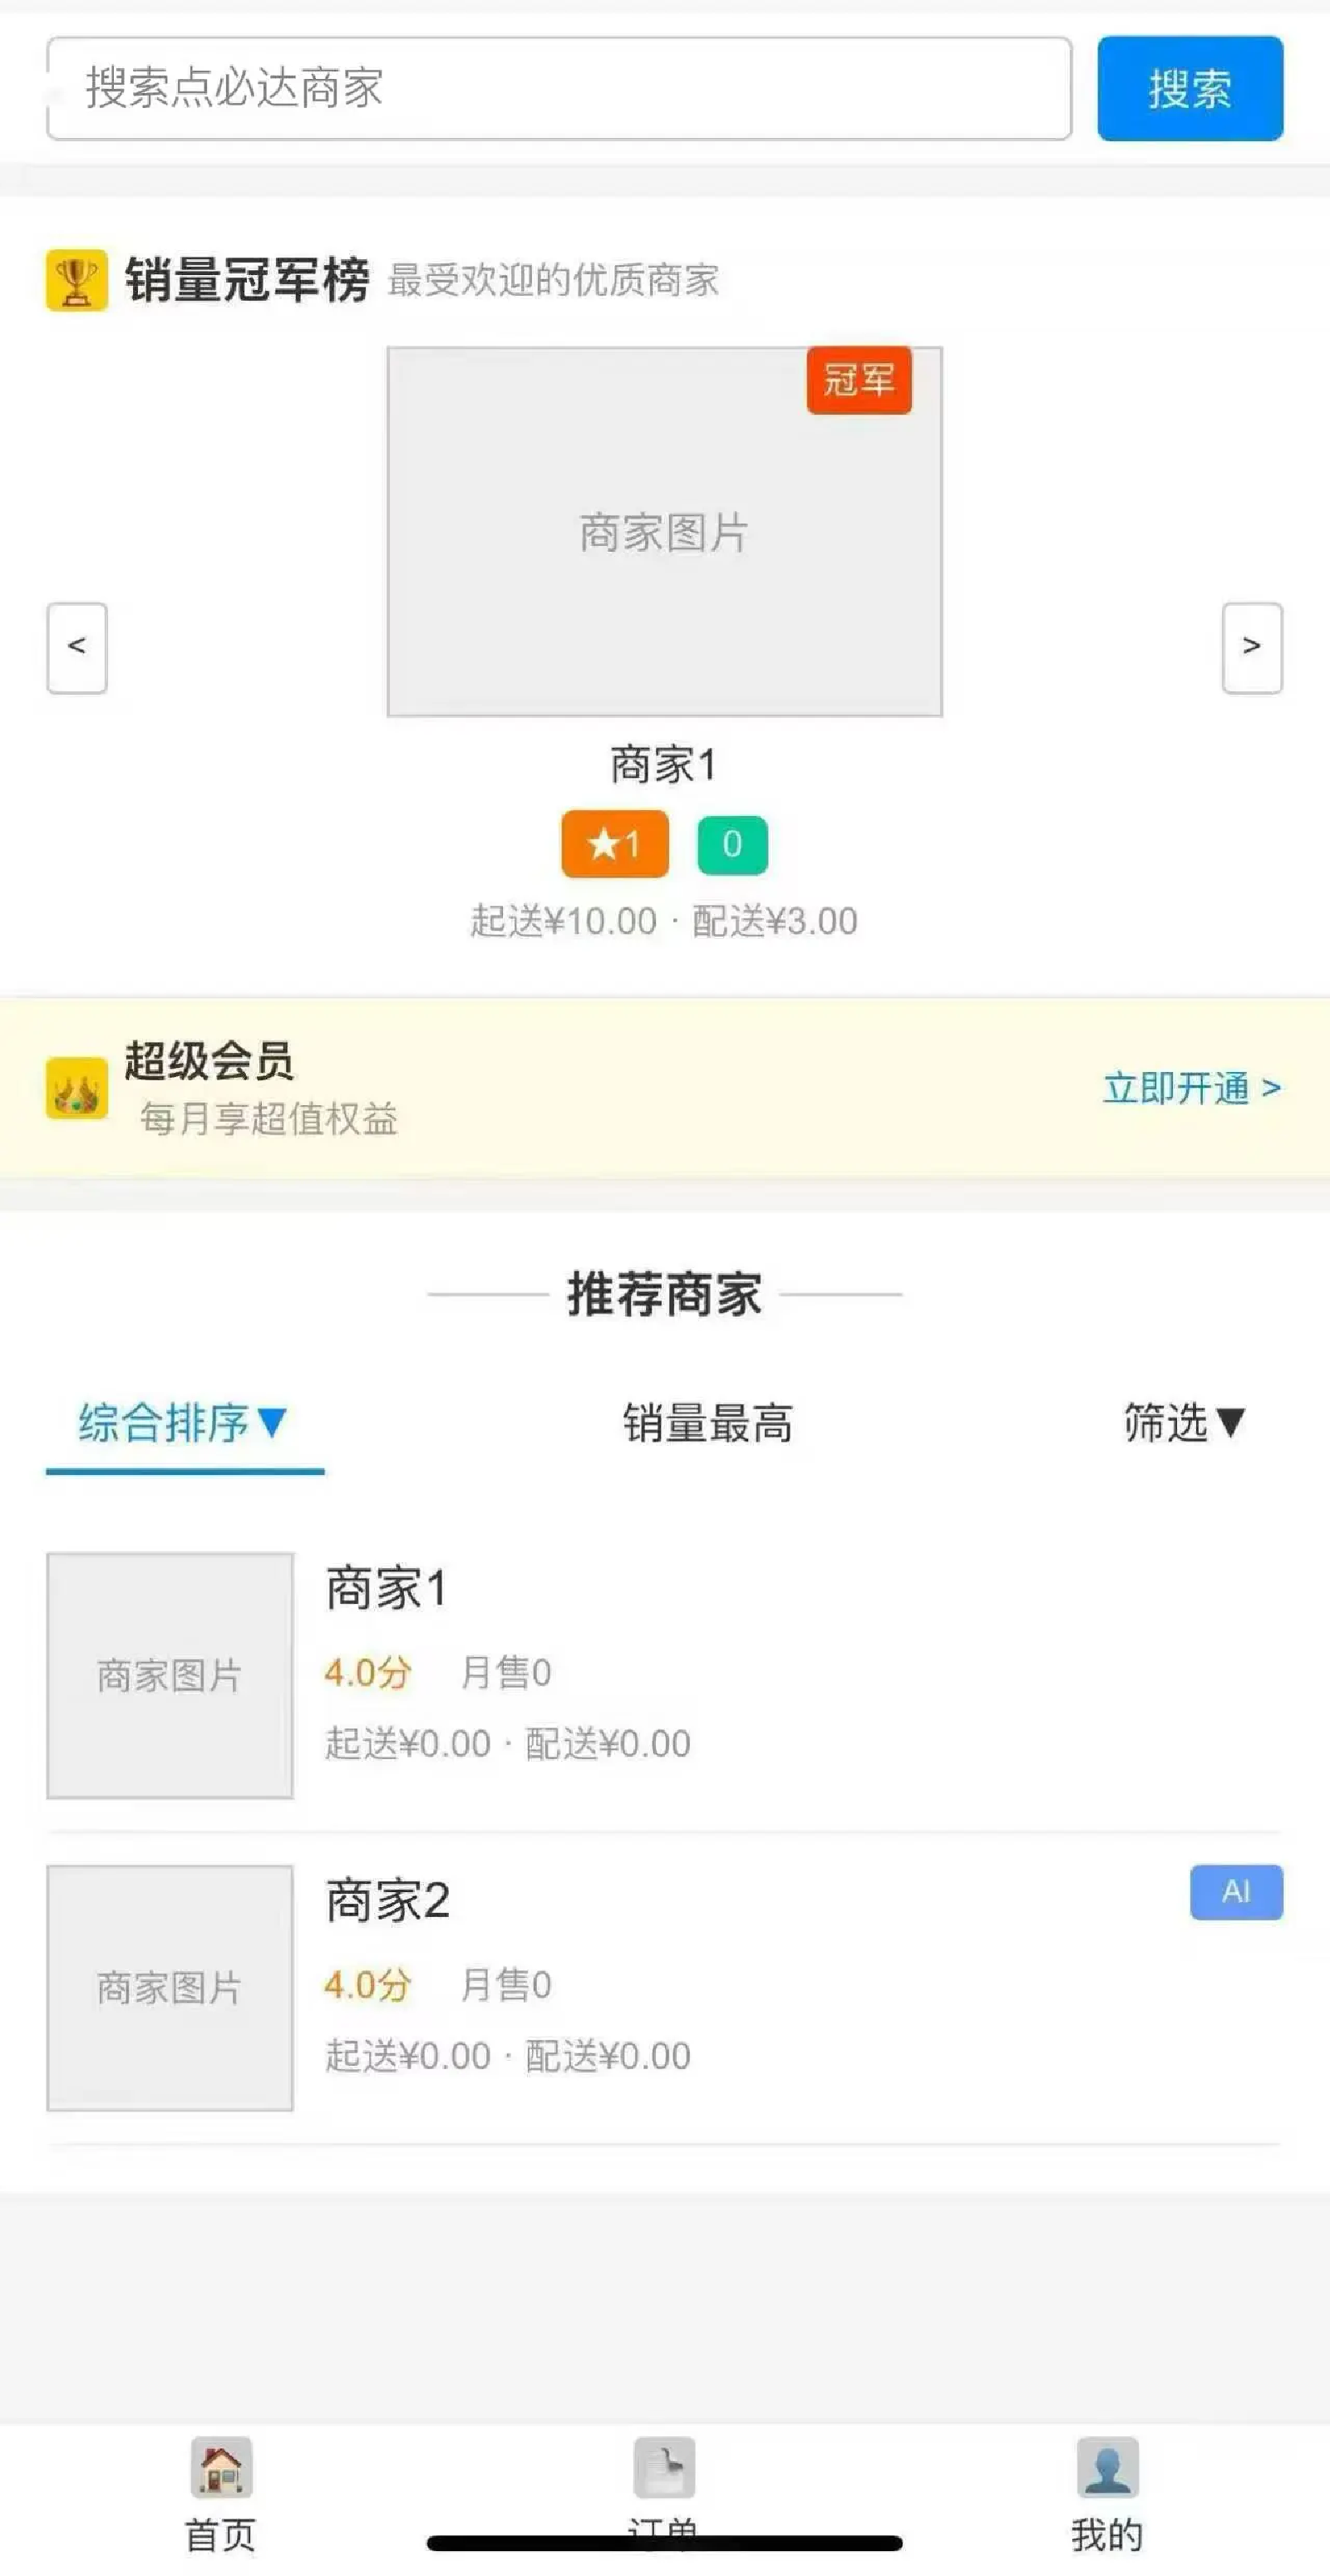
\includegraphics[width=0.8\linewidth]{figures/frontend/img1}
    \end{minipage}
    \hspace{1cm}
    \begin{minipage}[t]{0.35\linewidth}
        \centering
        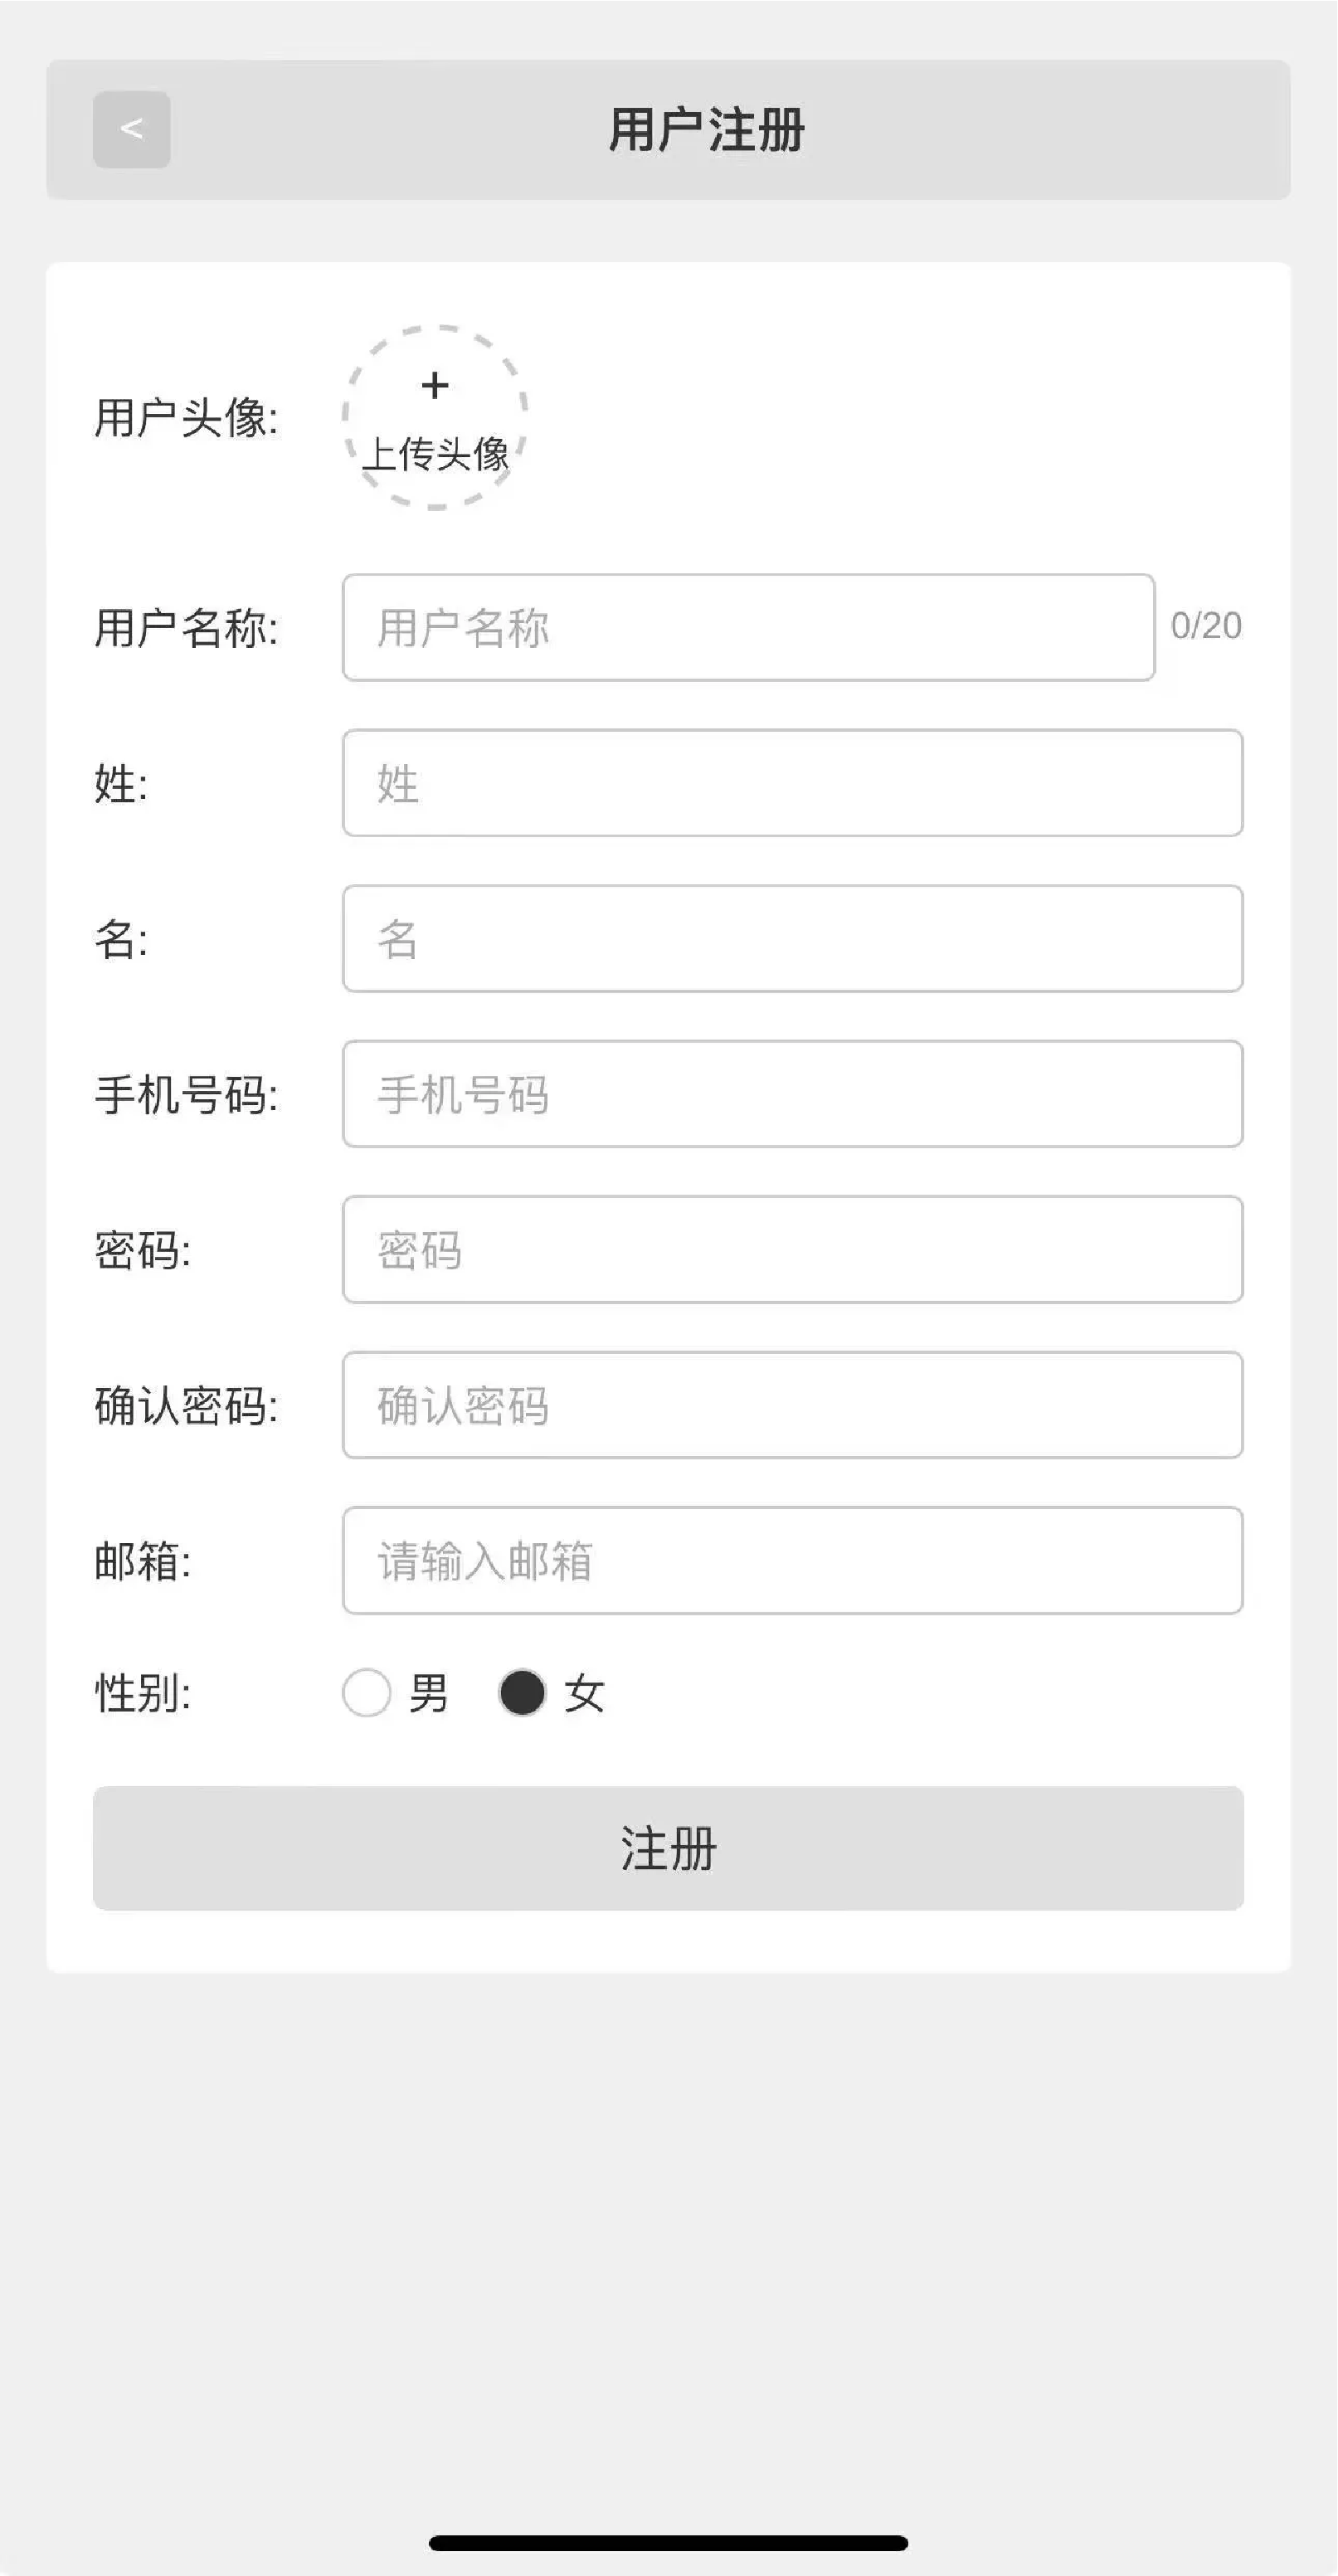
\includegraphics[width=0.8\linewidth]{figures/frontend/img2}
    \end{minipage}

    \hspace*{-1.5cm}

    \caption{首页 \& 用户注册界面}
    \label{fig:interfaces}
\end{figure}

\begin{figure}[H]
    \centering


    \hspace*{-1.5cm}

    \begin{minipage}[t]{0.35\linewidth}
        \centering
        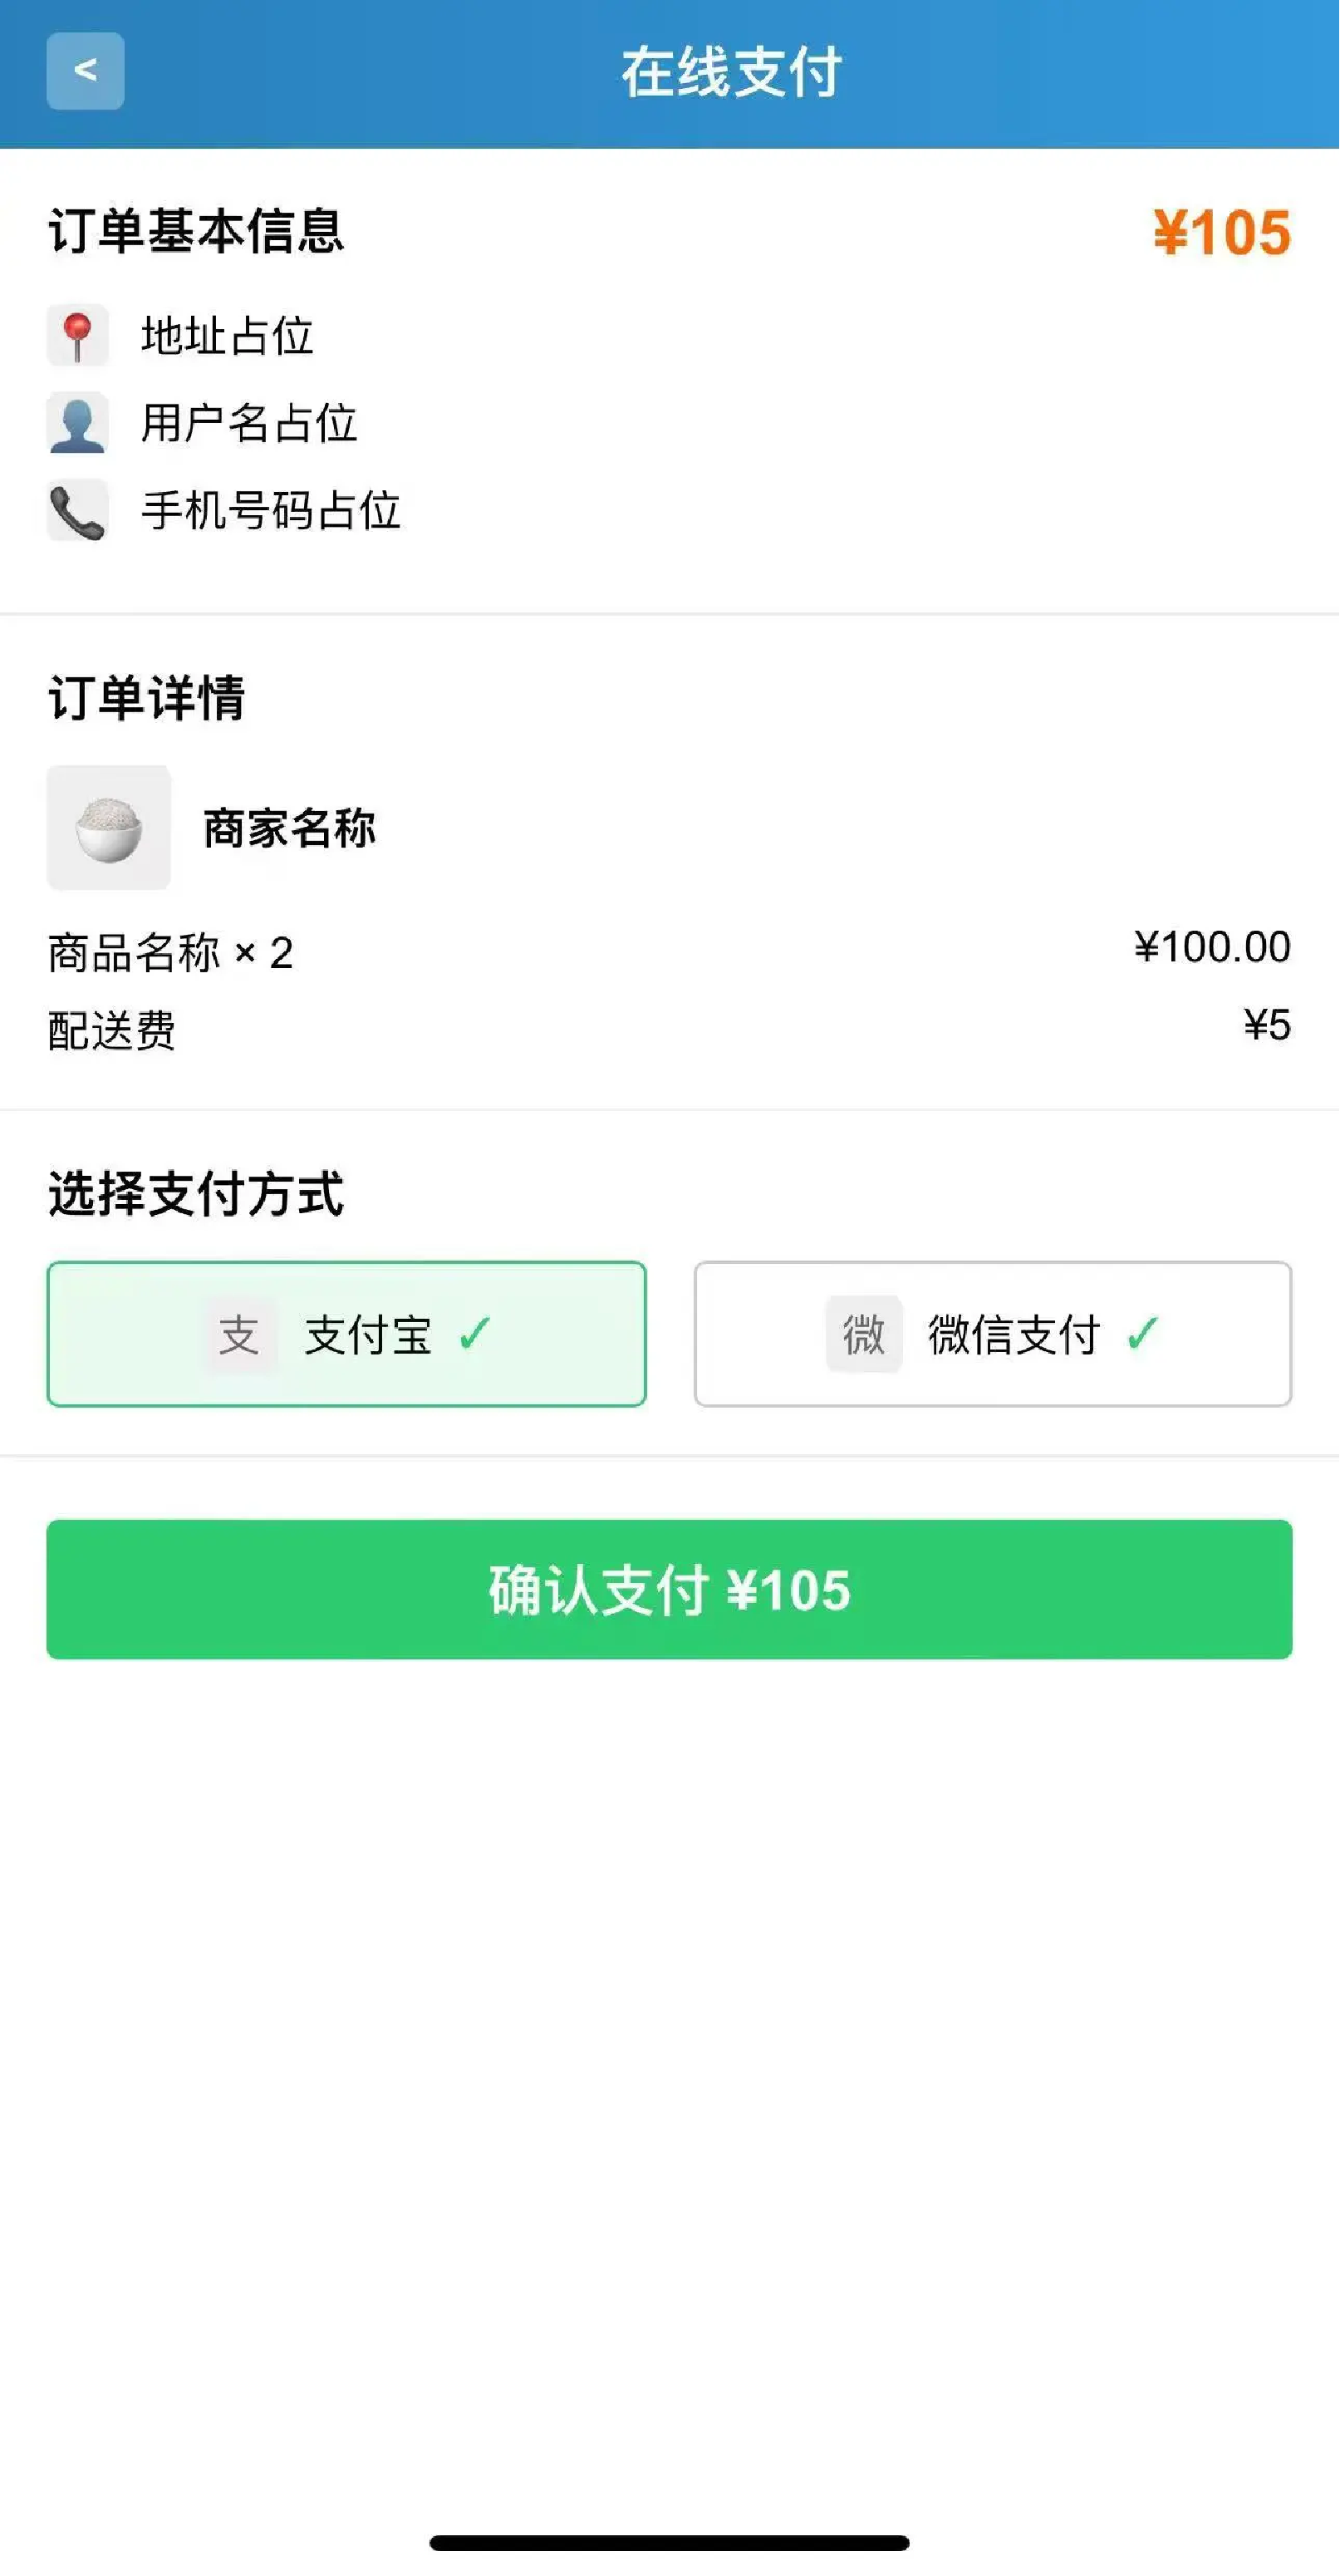
\includegraphics[width=0.8\linewidth]{figures/frontend/img3}
    \end{minipage}
    \hspace{1cm}
    \begin{minipage}[t]{0.35\linewidth}
        \centering
        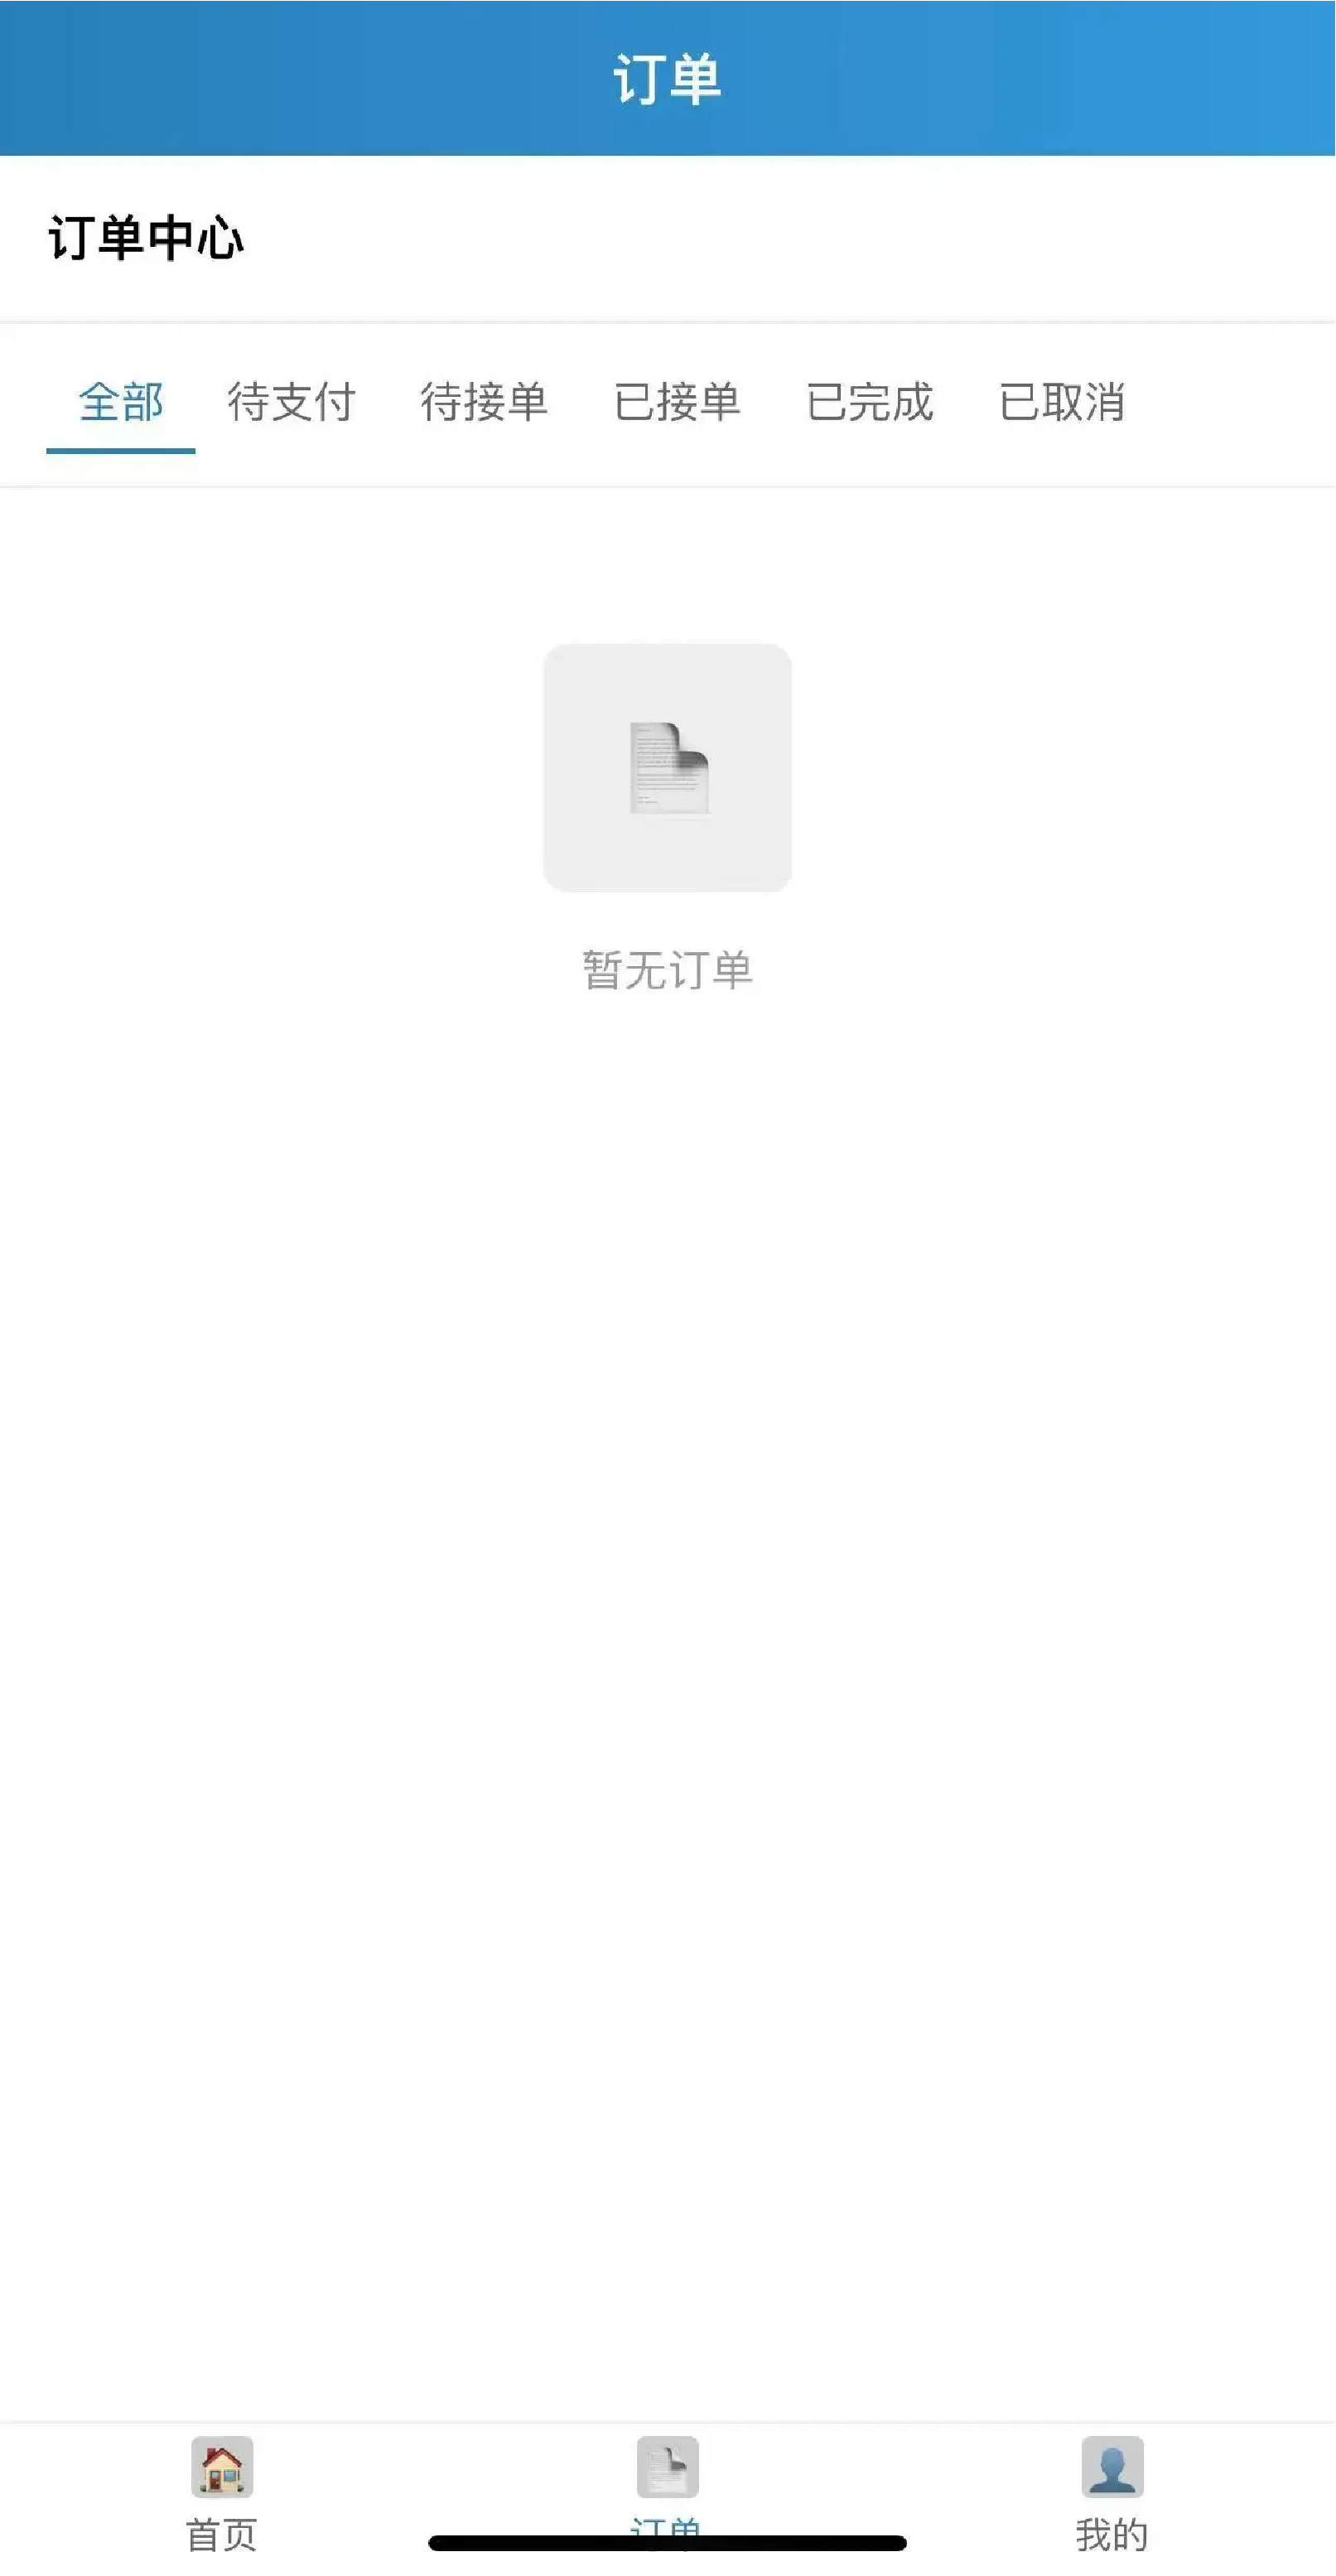
\includegraphics[width=0.8\linewidth]{figures/frontend/img4}
    \end{minipage}

    \hspace*{-1.5cm}

    \caption{支付页面 \& 顾客订单页面}
    \label{fig:interfaces}
\end{figure}

\begin{figure}[H]
    \centering


    \hspace*{-1.5cm}

    \begin{minipage}[t]{0.35\linewidth}
        \centering
        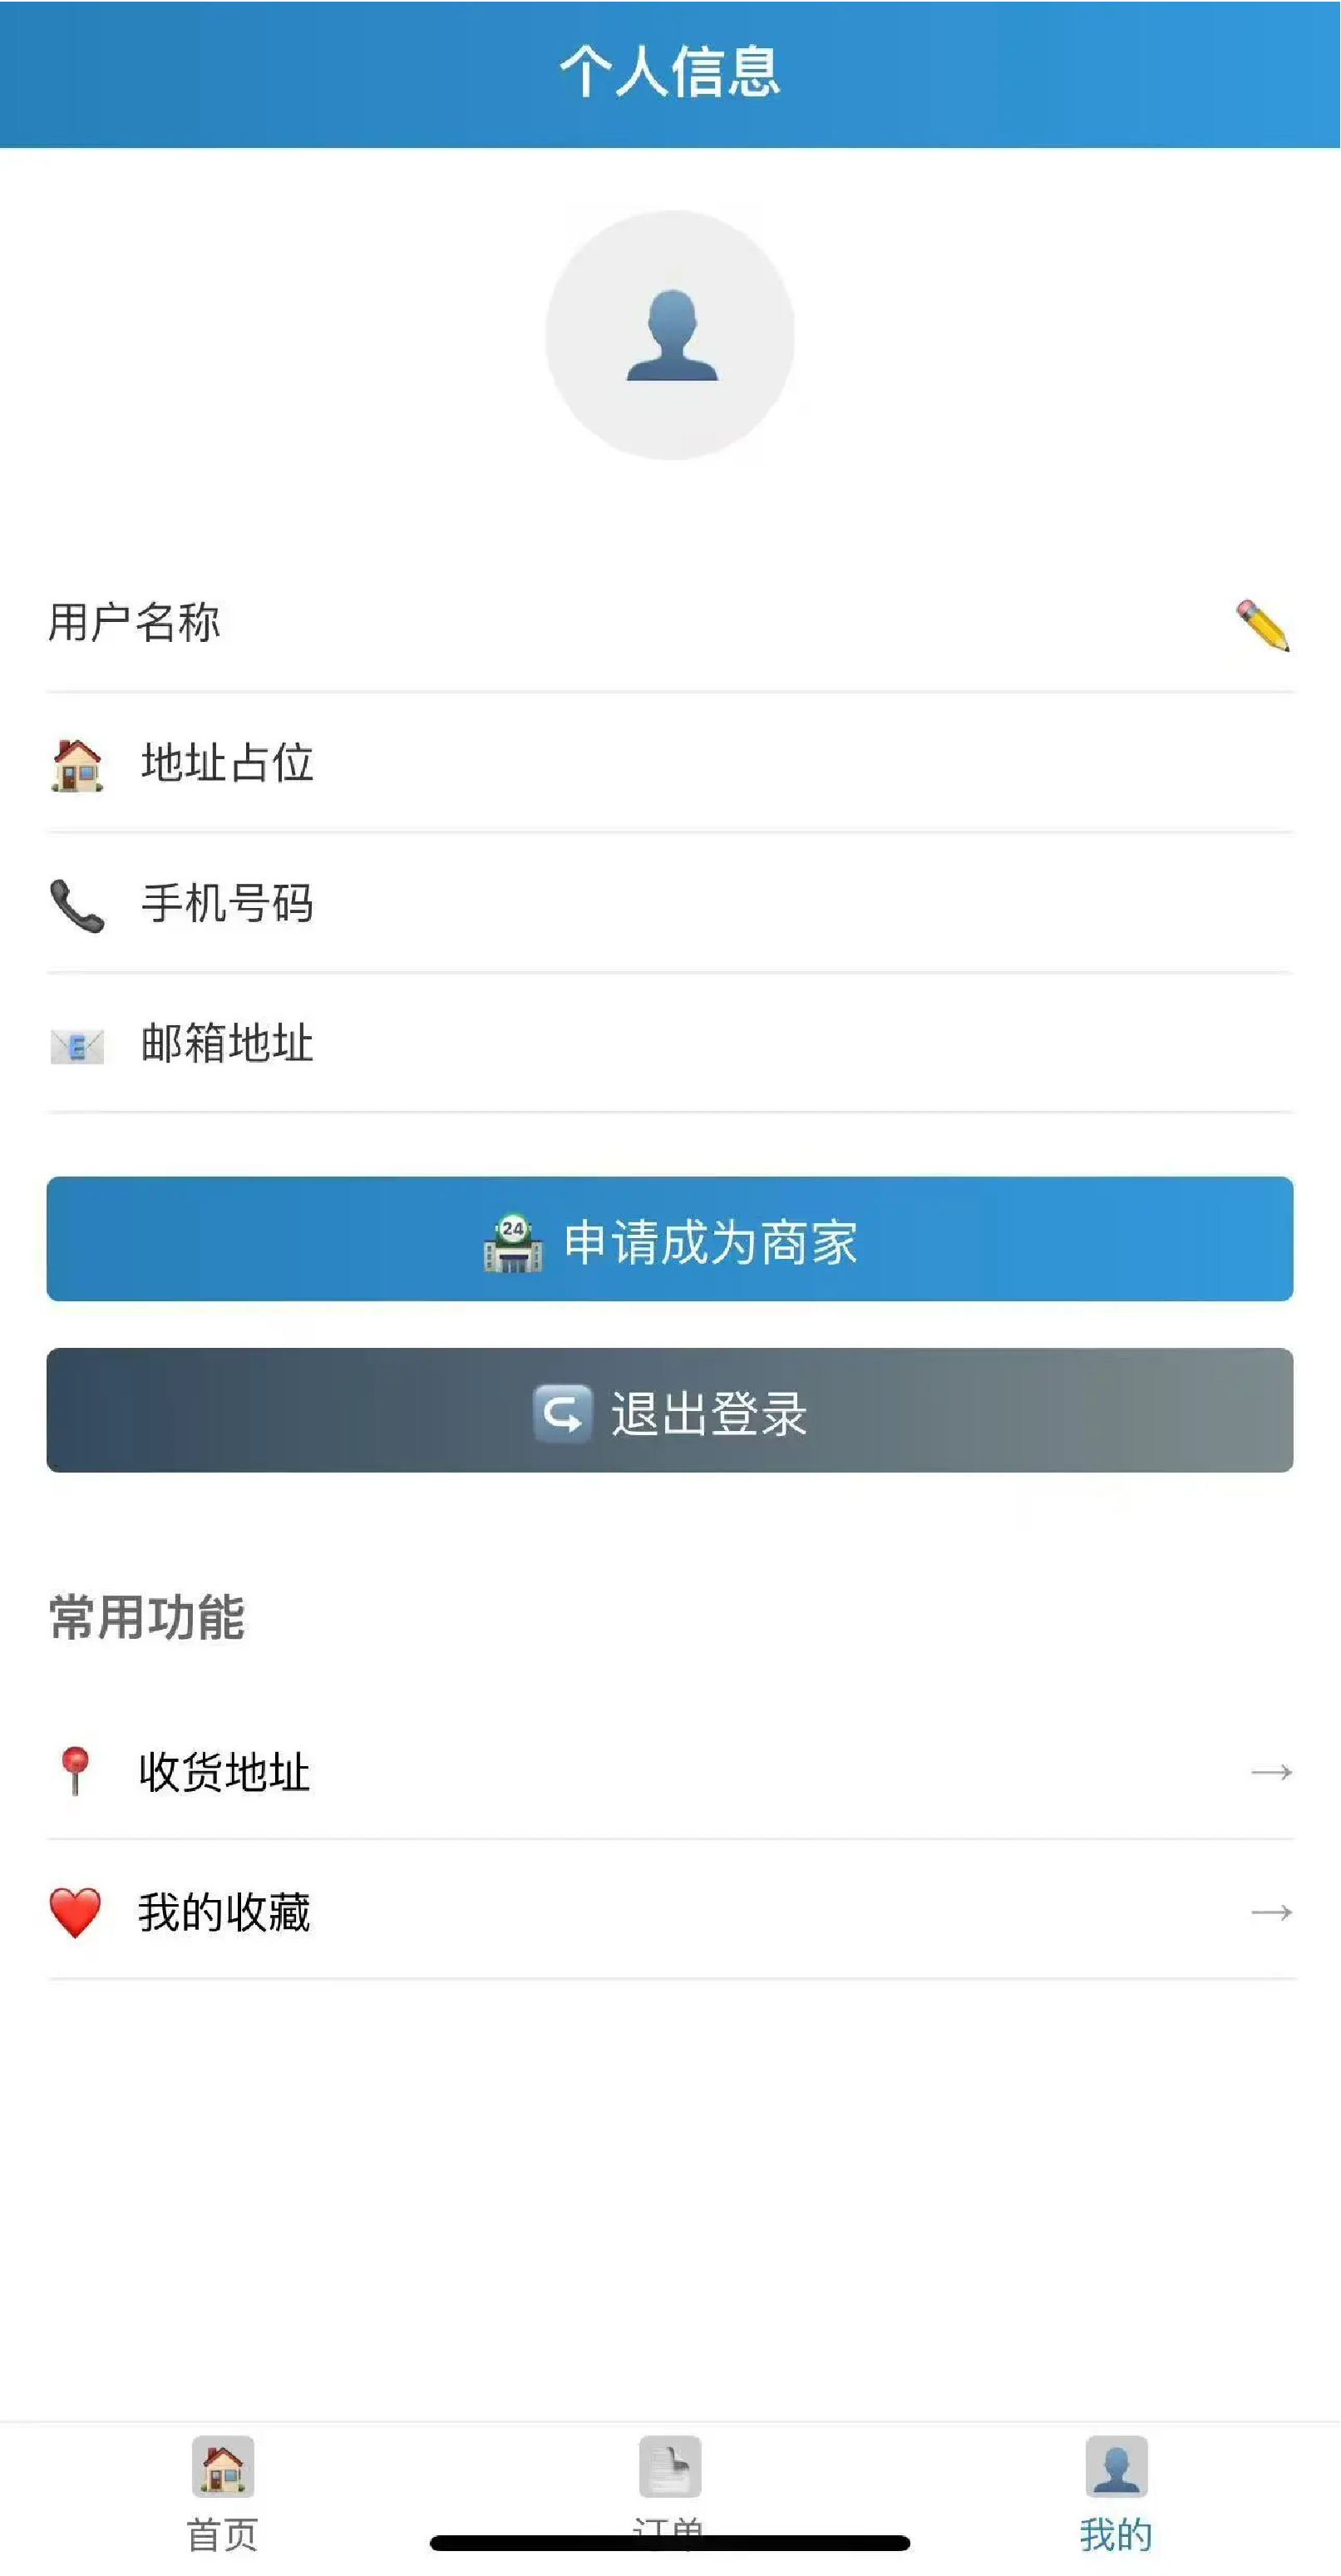
\includegraphics[width=0.8\linewidth]{figures/frontend/img5}
    \end{minipage}
    \hspace{1cm}
    \begin{minipage}[t]{0.35\linewidth}
        \centering
        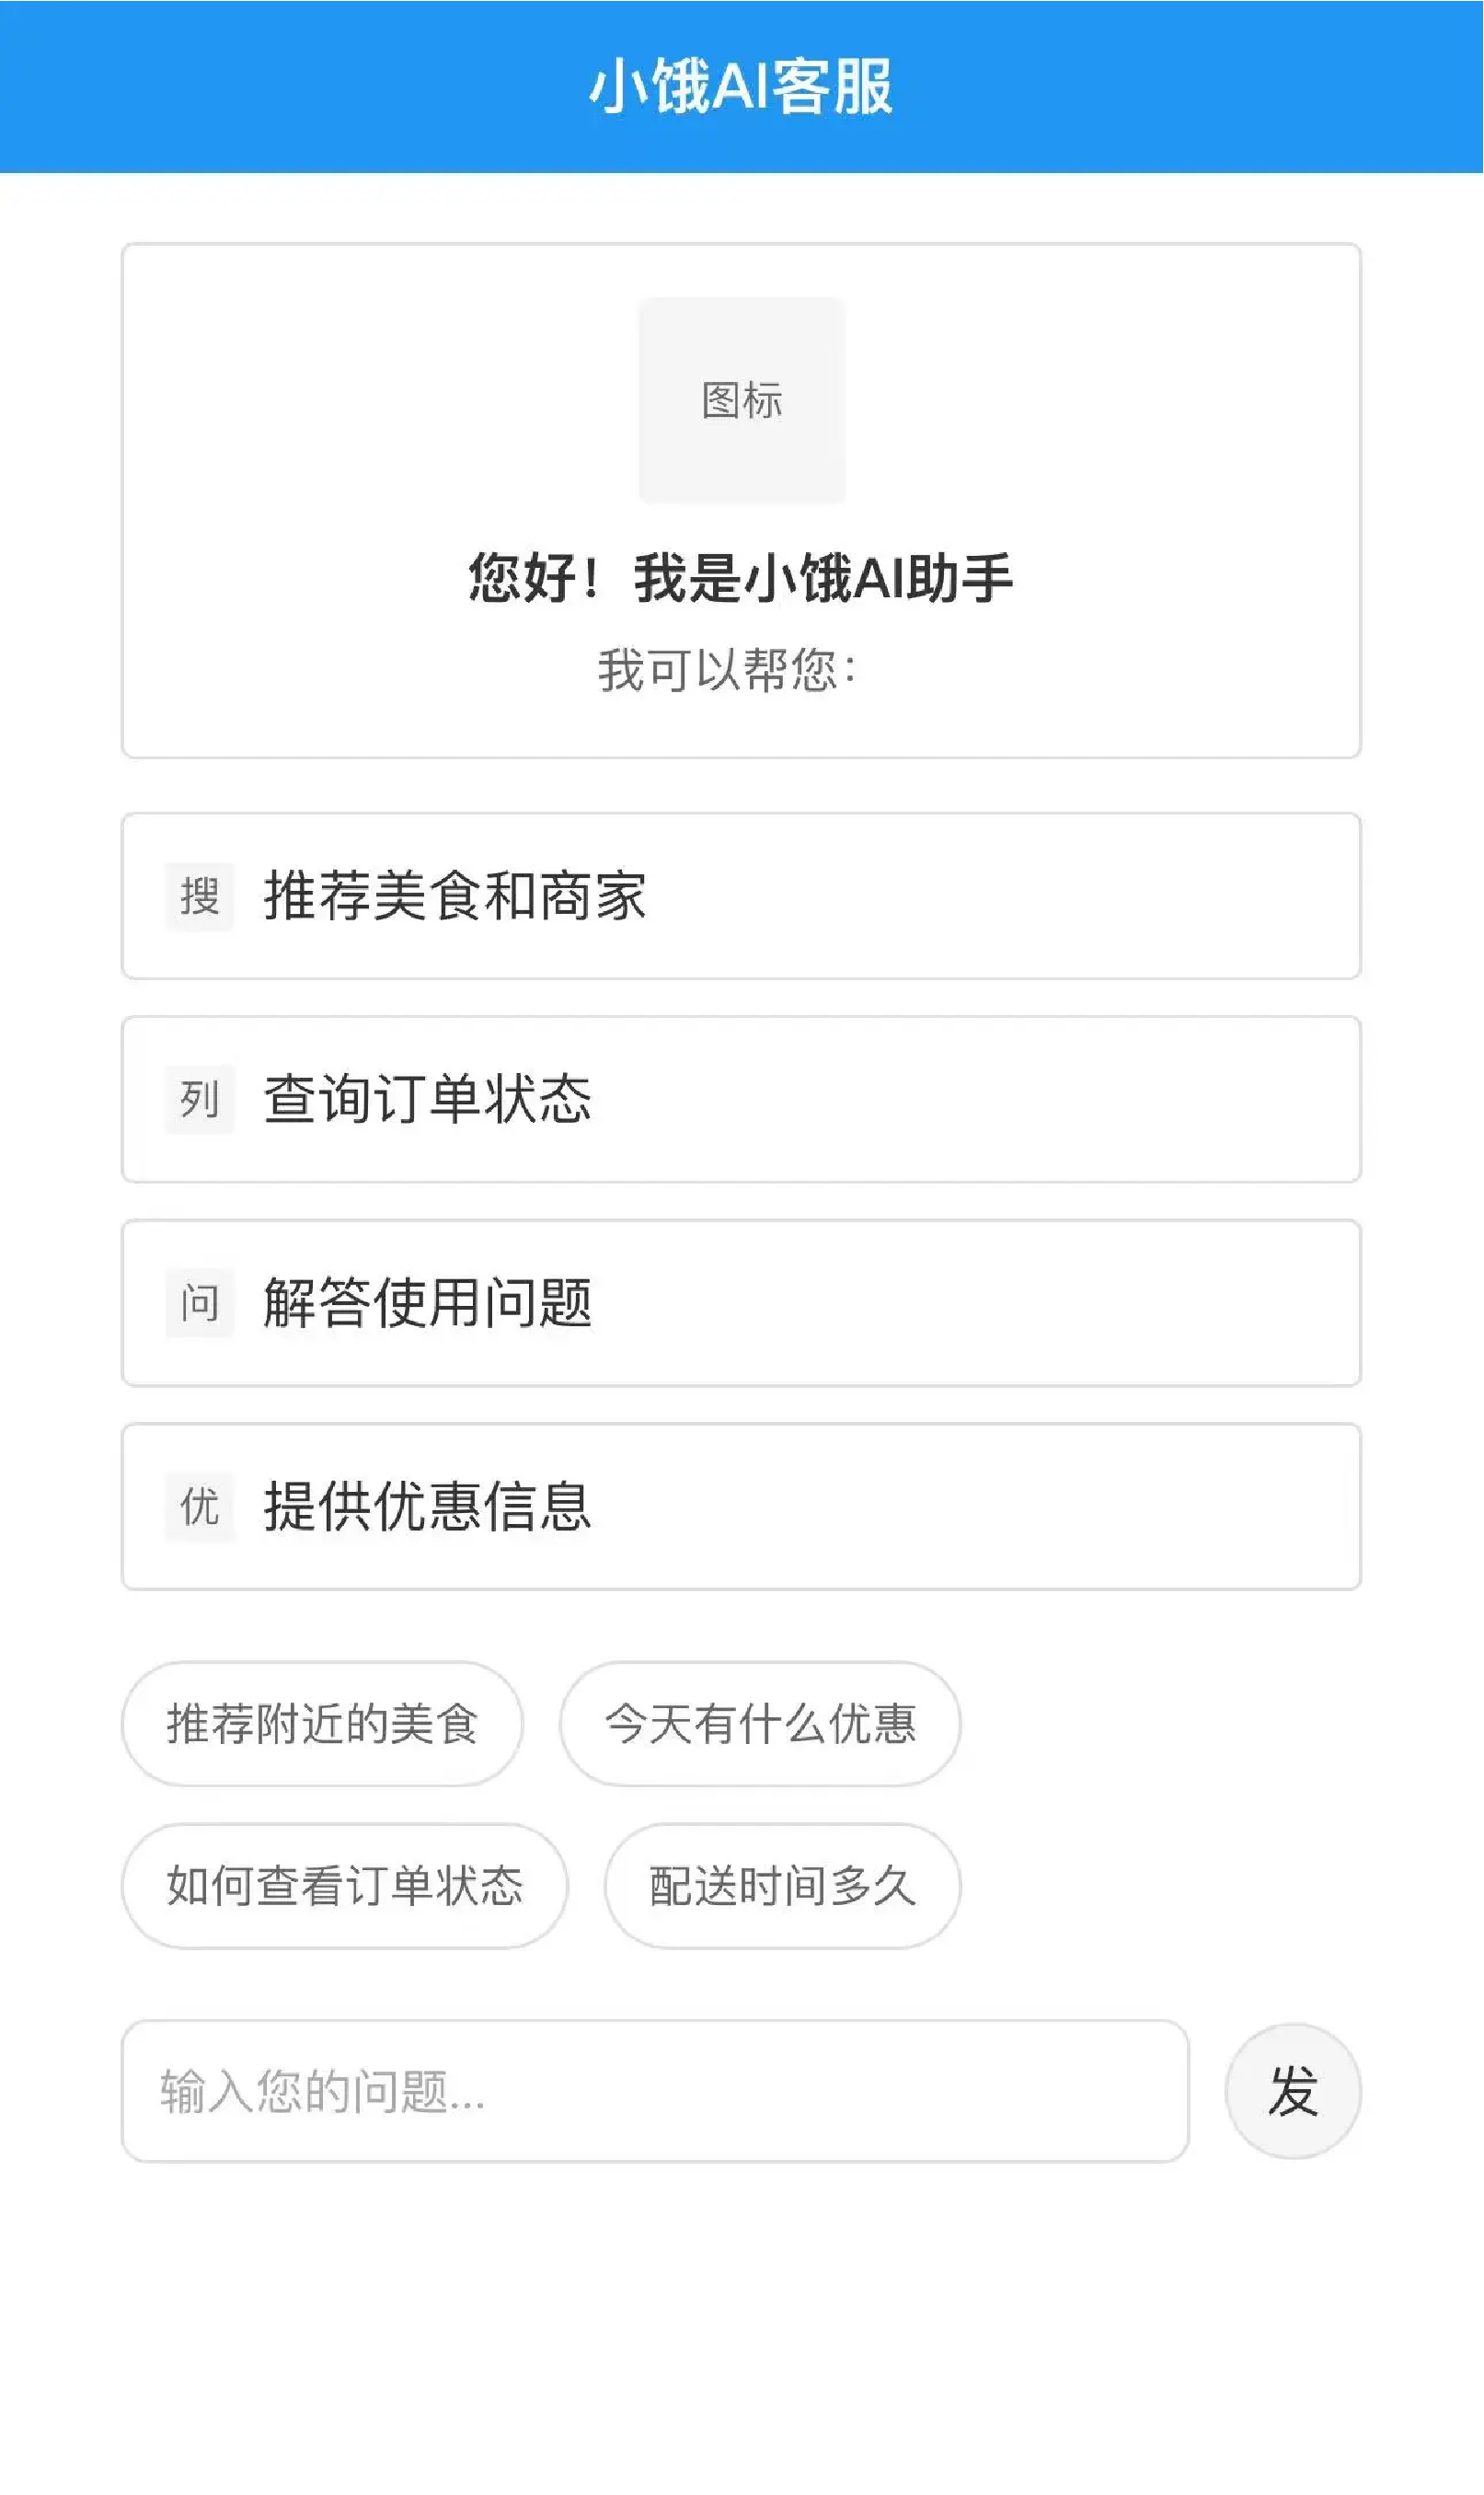
\includegraphics[width=0.8\linewidth]{figures/frontend/img6}
    \end{minipage}

    \hspace*{-1.5cm}

    \caption{支付页面 \& 顾客订单页面}
    \label{fig:interfaces}
\end{figure}

\newpage


\textbf{2. 商家端界面}

\begin{figure}[H]
    \centering


    \hspace*{-1.5cm}

    \begin{minipage}[t]{0.35\linewidth}
        \centering
        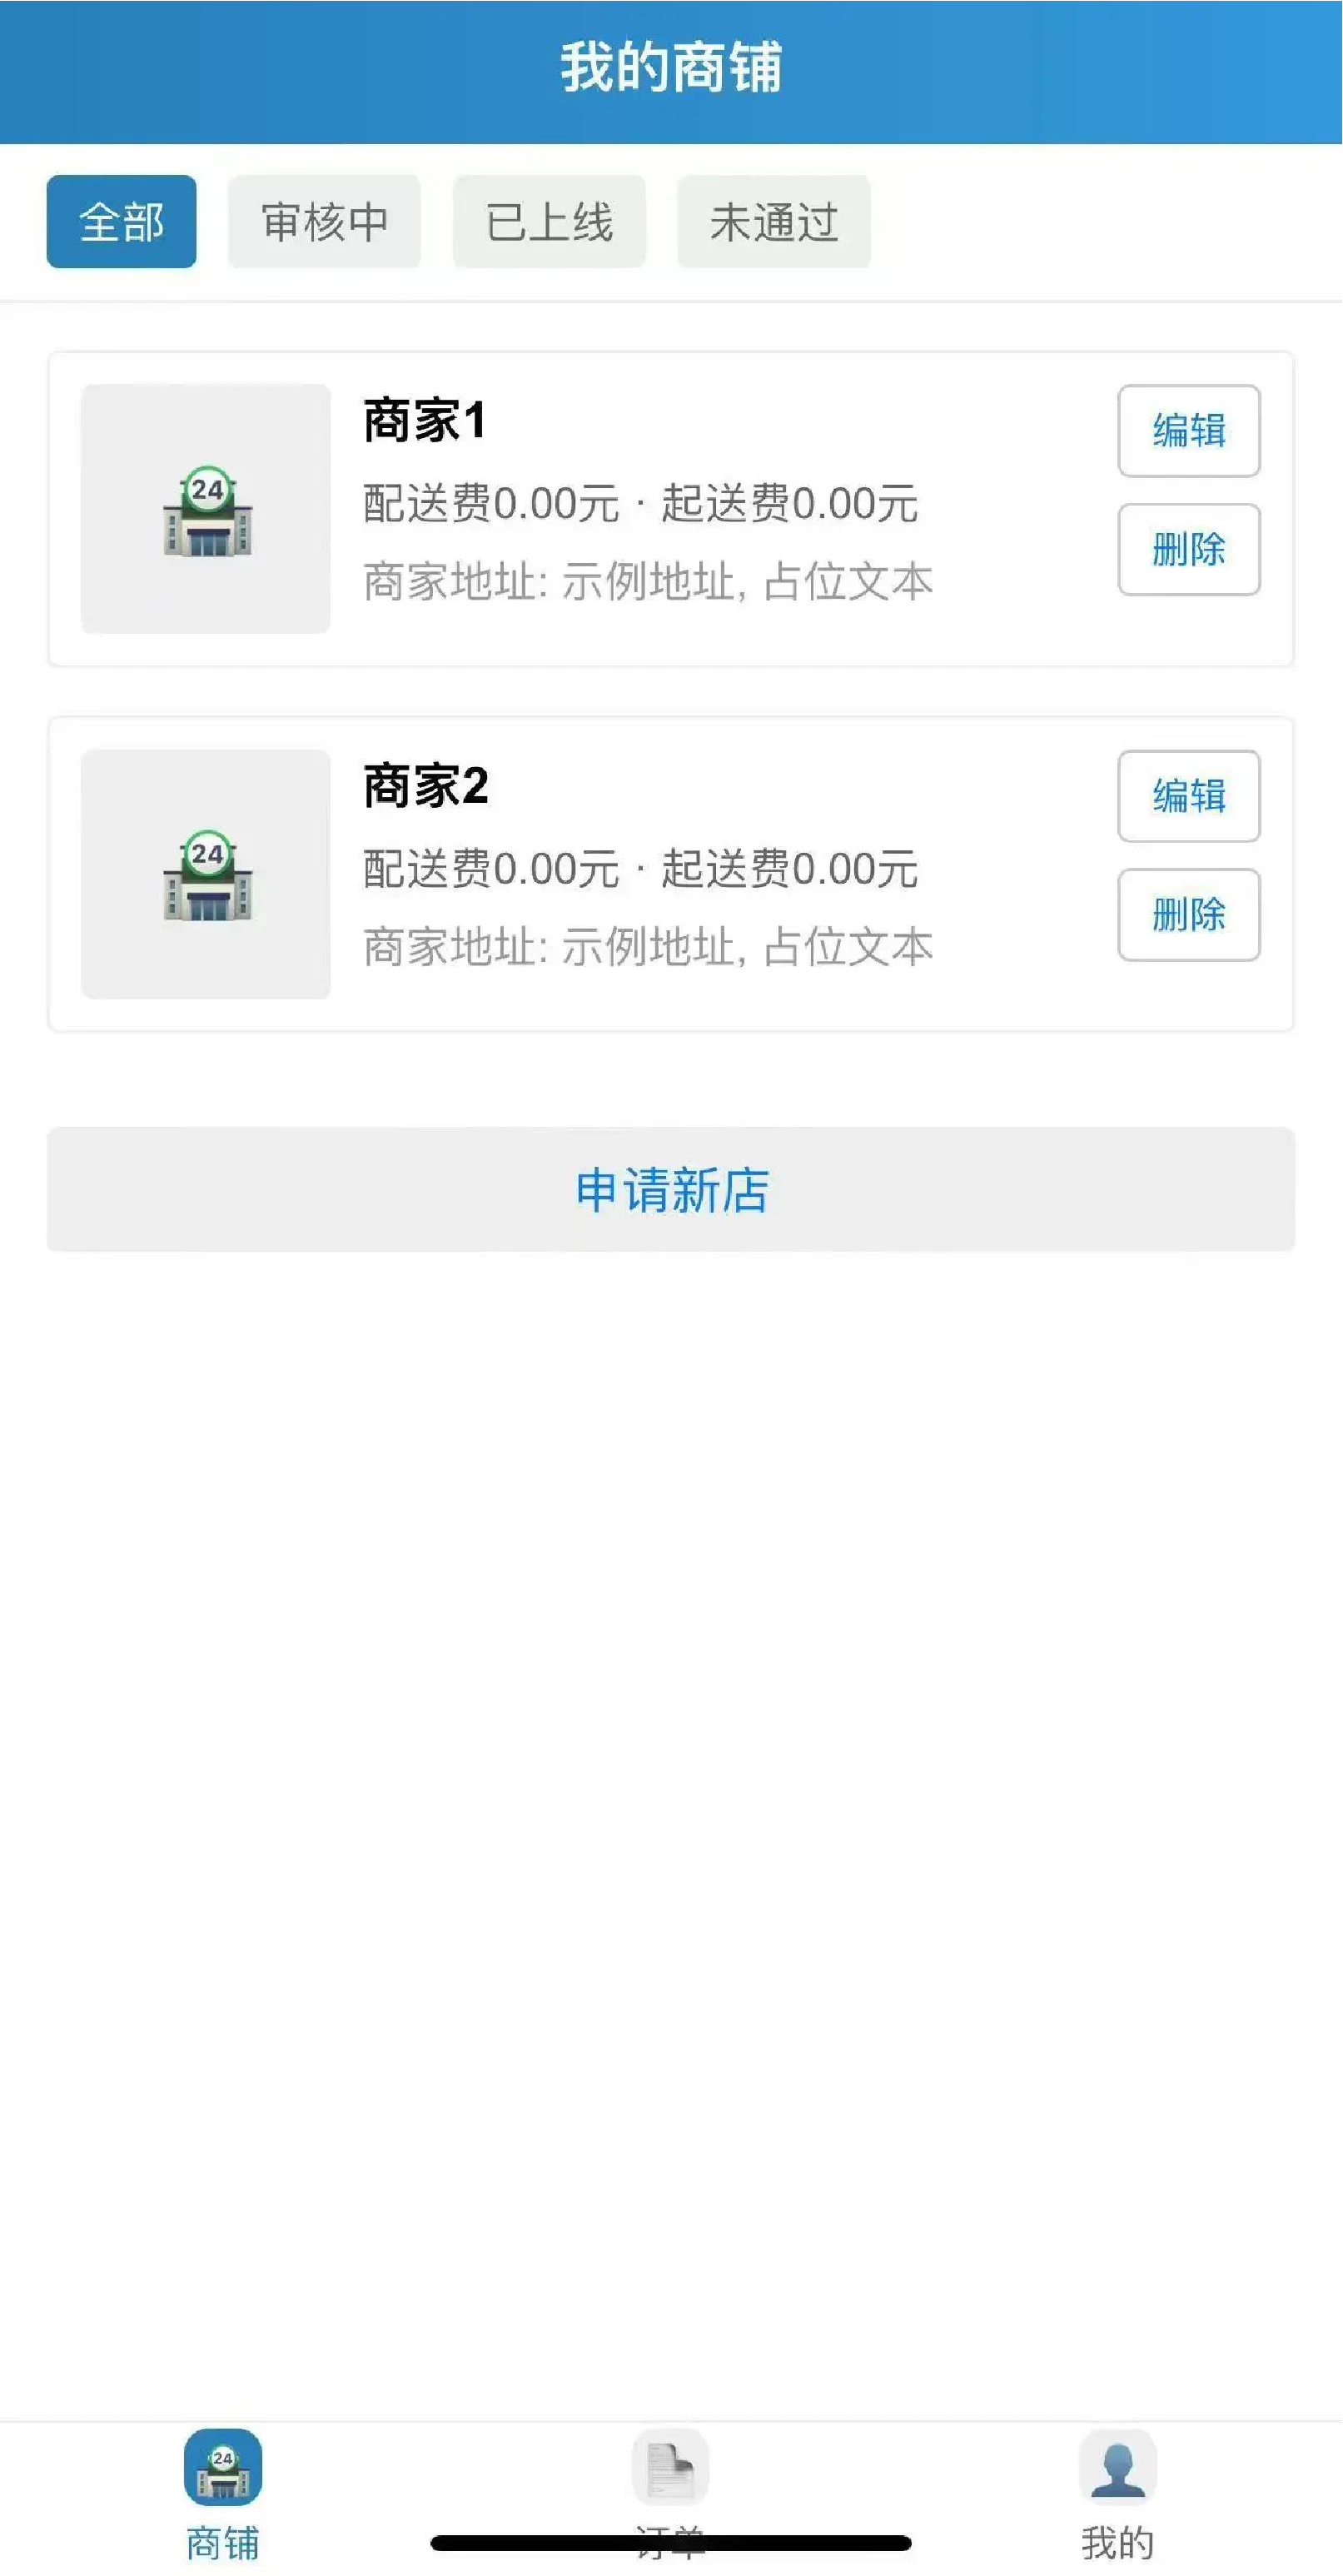
\includegraphics[width=0.8\linewidth]{figures/frontend/img10}
    \end{minipage}
    \hspace{1cm}
    \begin{minipage}[t]{0.35\linewidth}
        \centering
        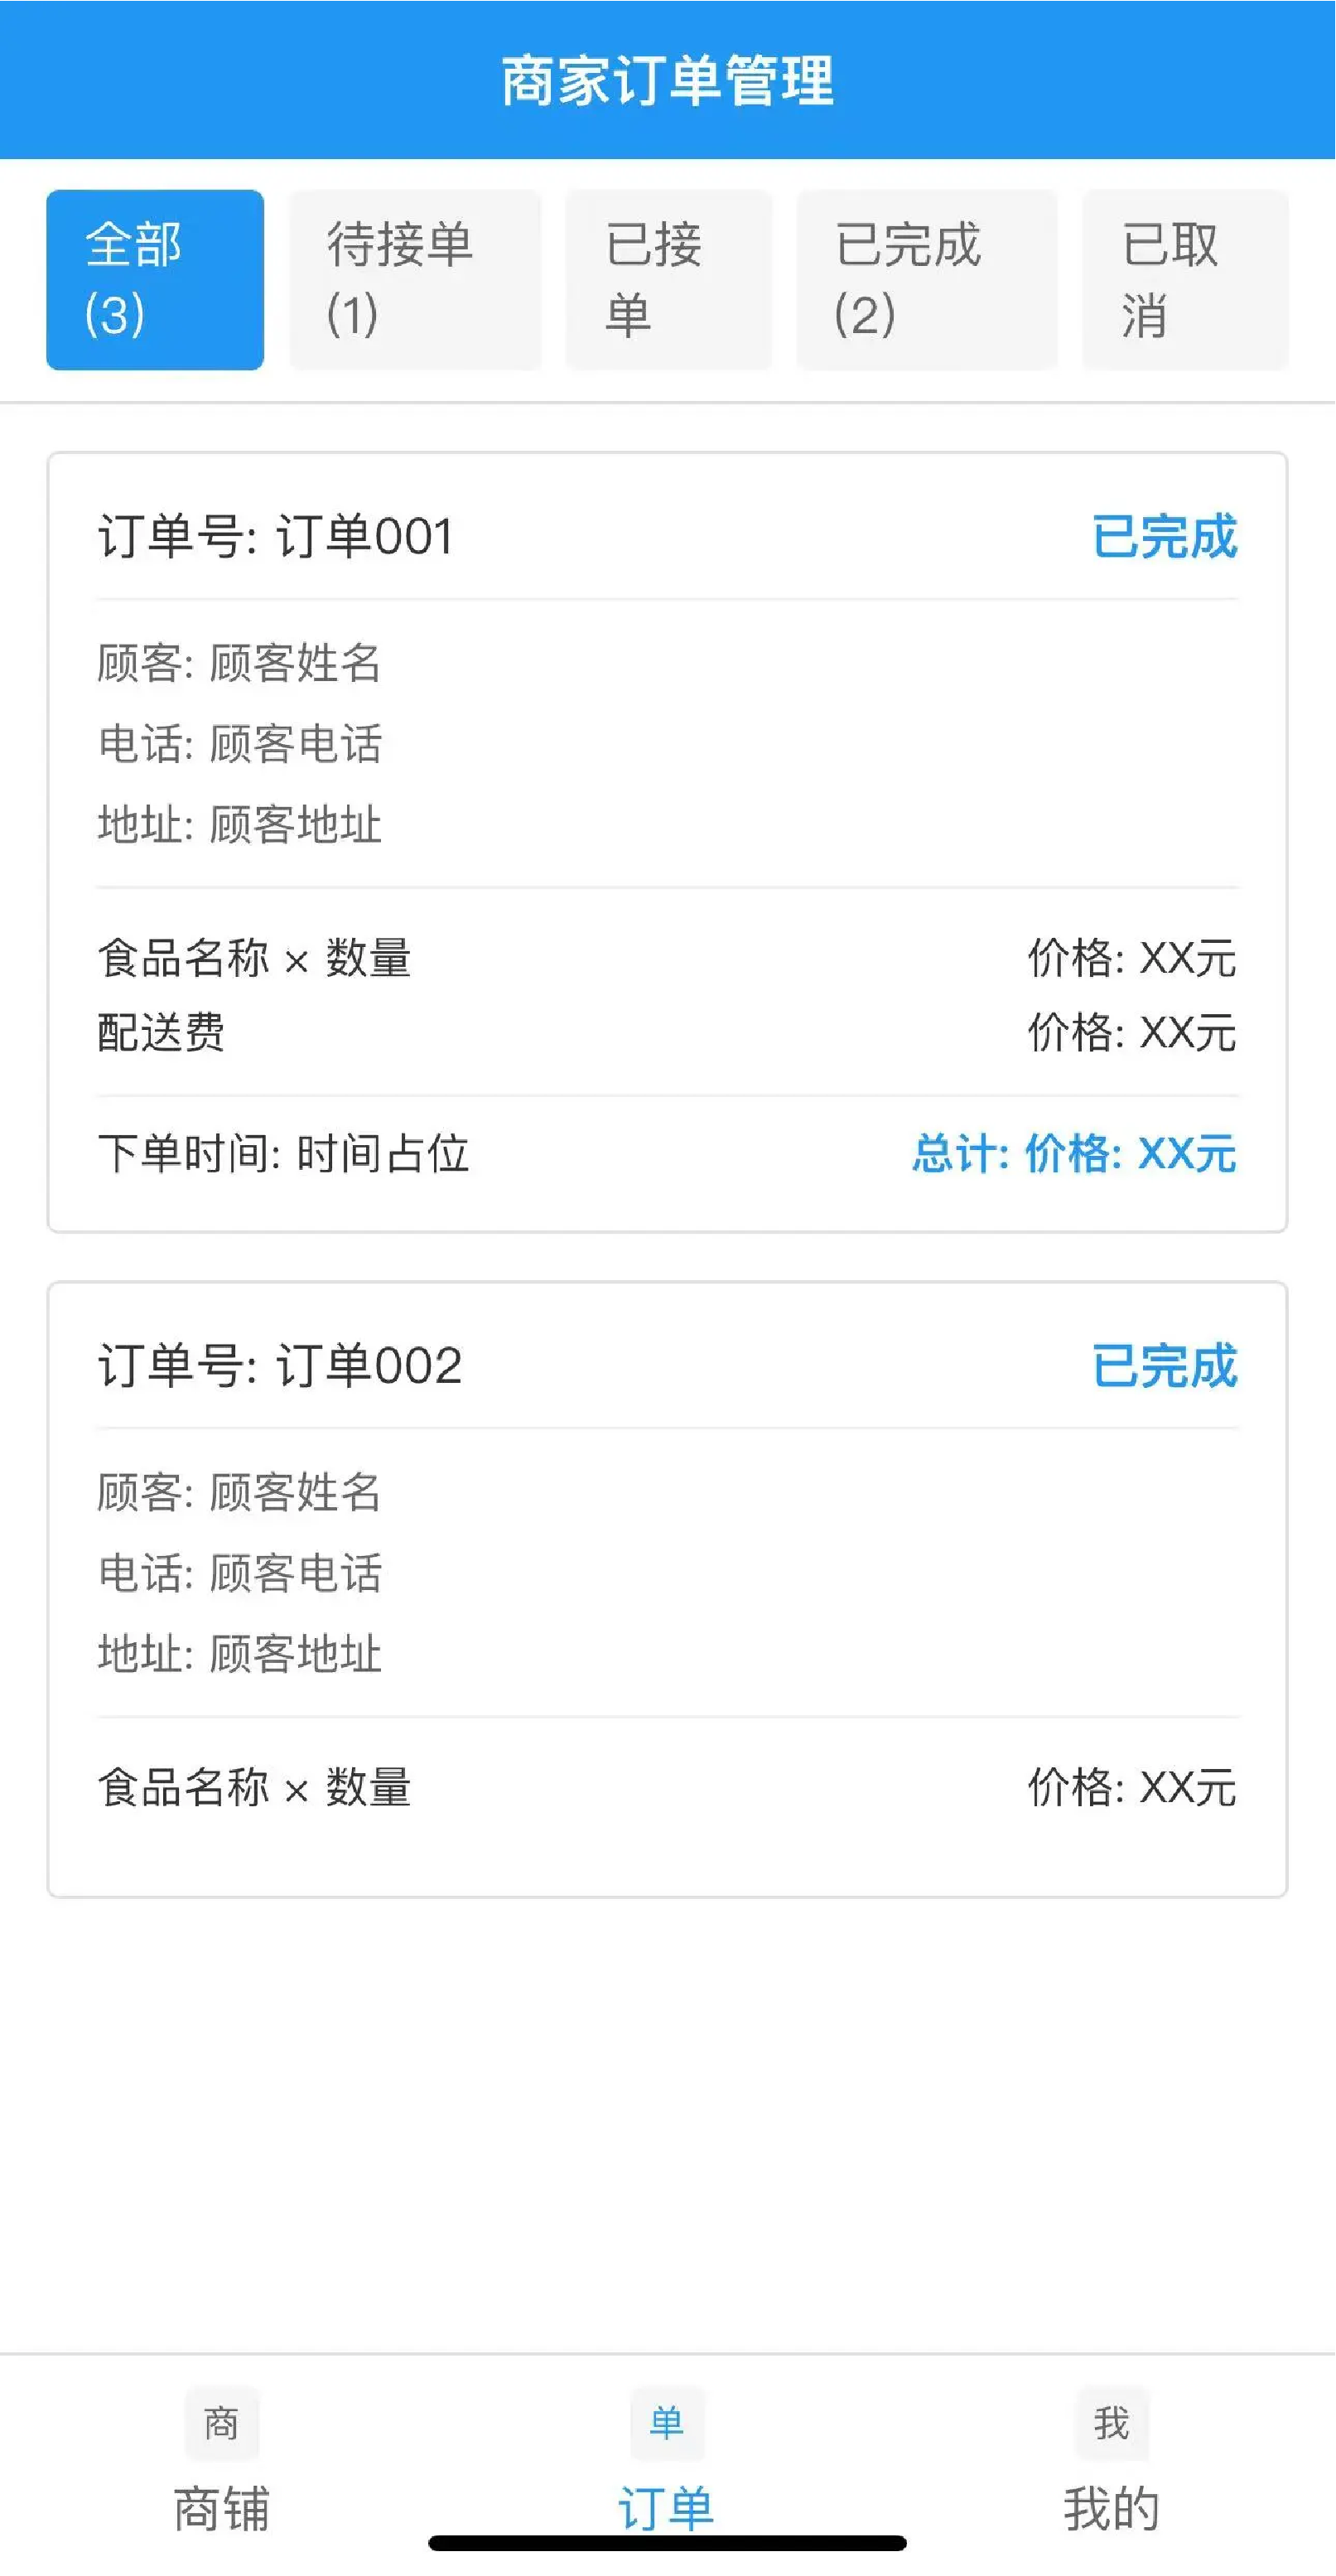
\includegraphics[width=0.8\linewidth]{figures/frontend/img9}
    \end{minipage}

    \hspace*{-1.5cm}

    \caption{我的商铺页面 \& 商家订单页面}
    \label{fig:interfaces}
\end{figure}

\begin{figure}[H]
    \centering
    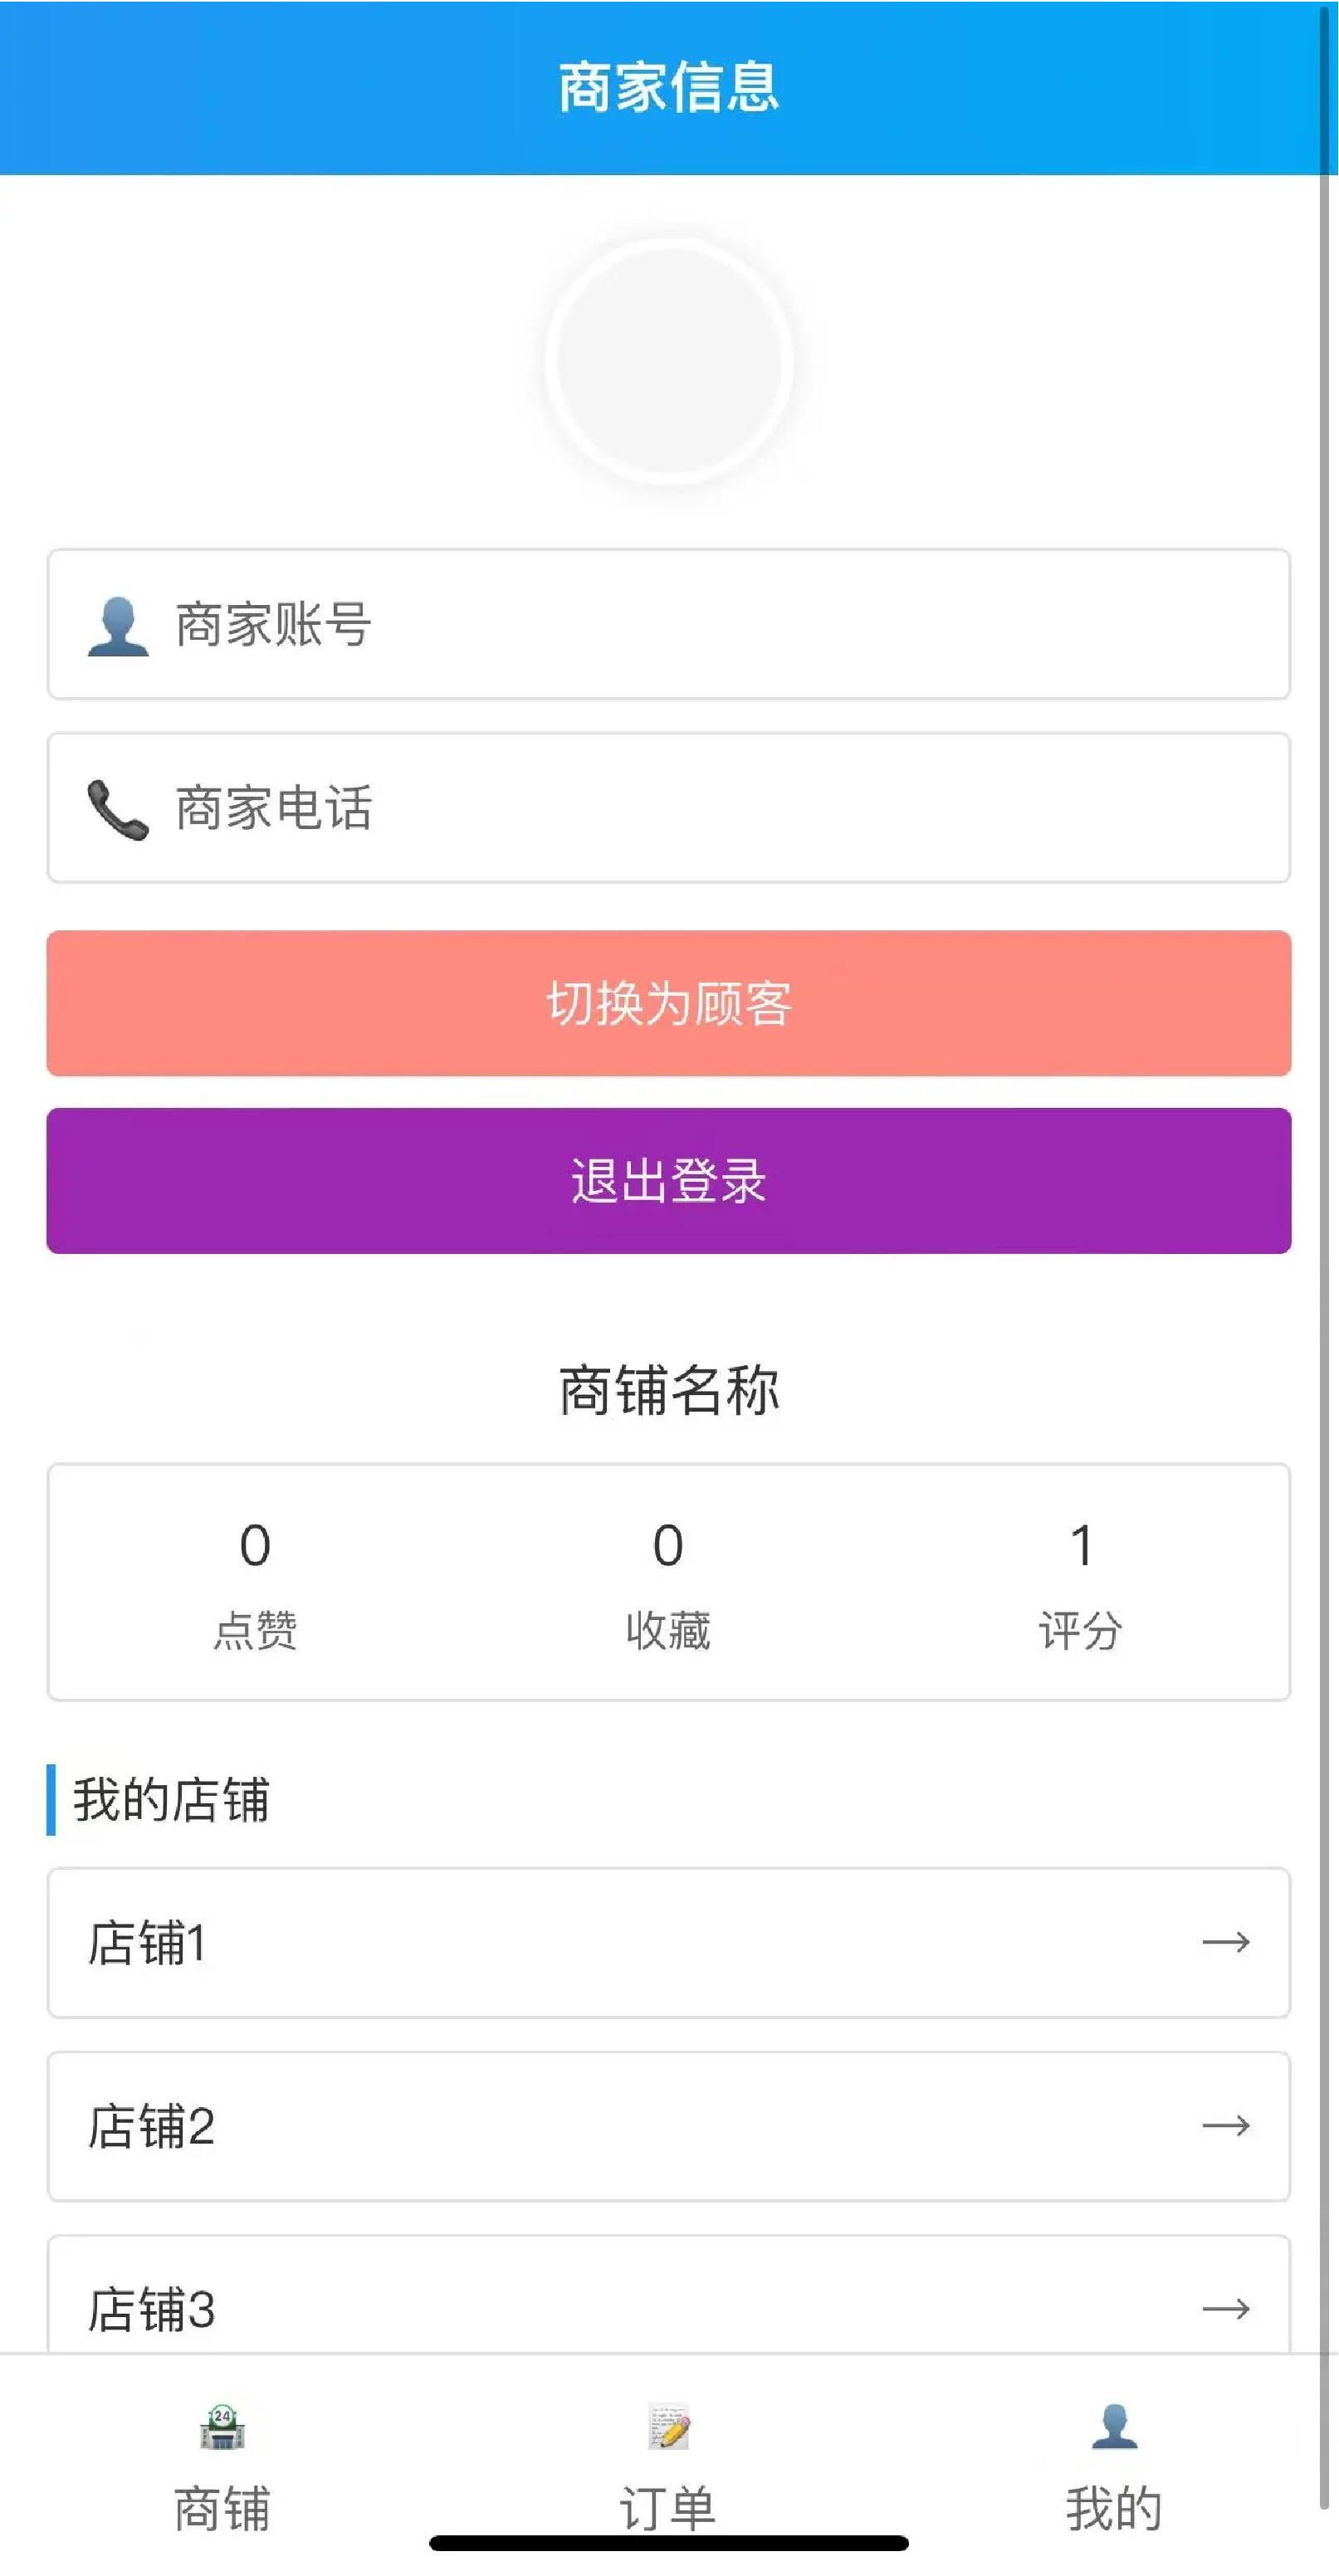
\includegraphics[width=0.3\textwidth]{figures/frontend/img11}
    \caption{商家信息页面}\label{fig:xml}
    \vspace{\baselineskip}
\end{figure}


\textbf{3. 管理端界面}

\begin{figure}[H]
    \centering


    \hspace*{-1.5cm}

    \begin{minipage}[t]{0.35\linewidth}
        \centering
        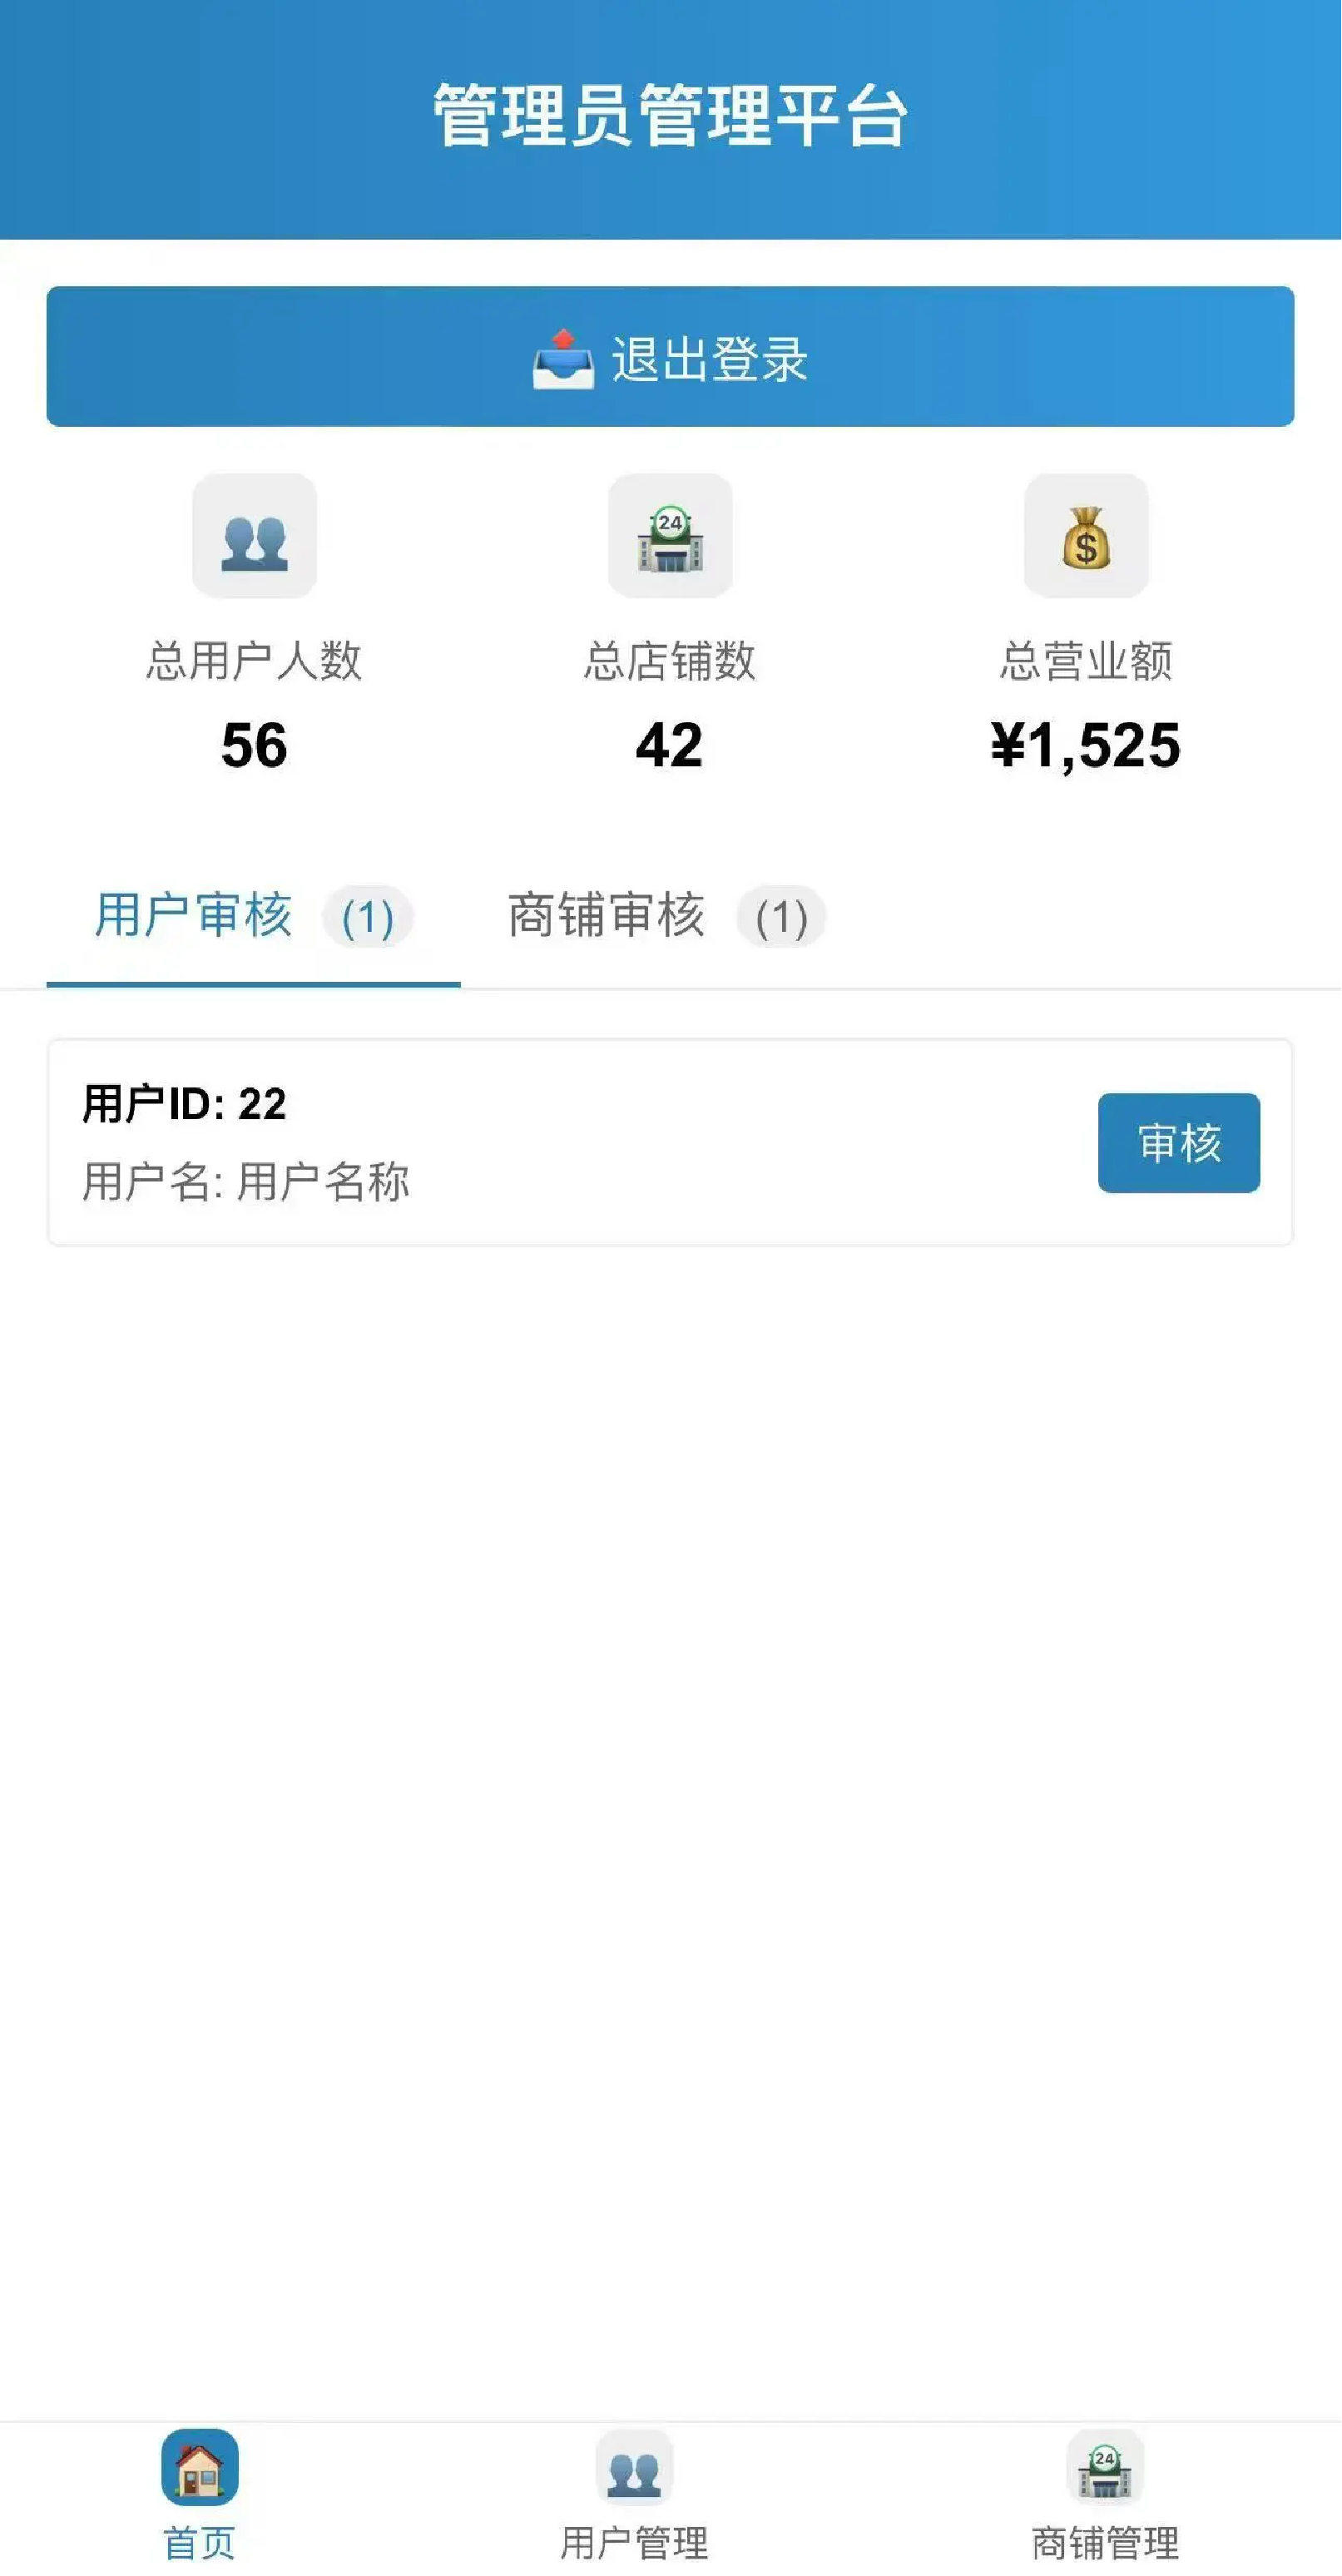
\includegraphics[width=0.8\linewidth]{figures/frontend/img7}
    \end{minipage}
    \hspace{1cm}
    \begin{minipage}[t]{0.35\linewidth}
        \centering
        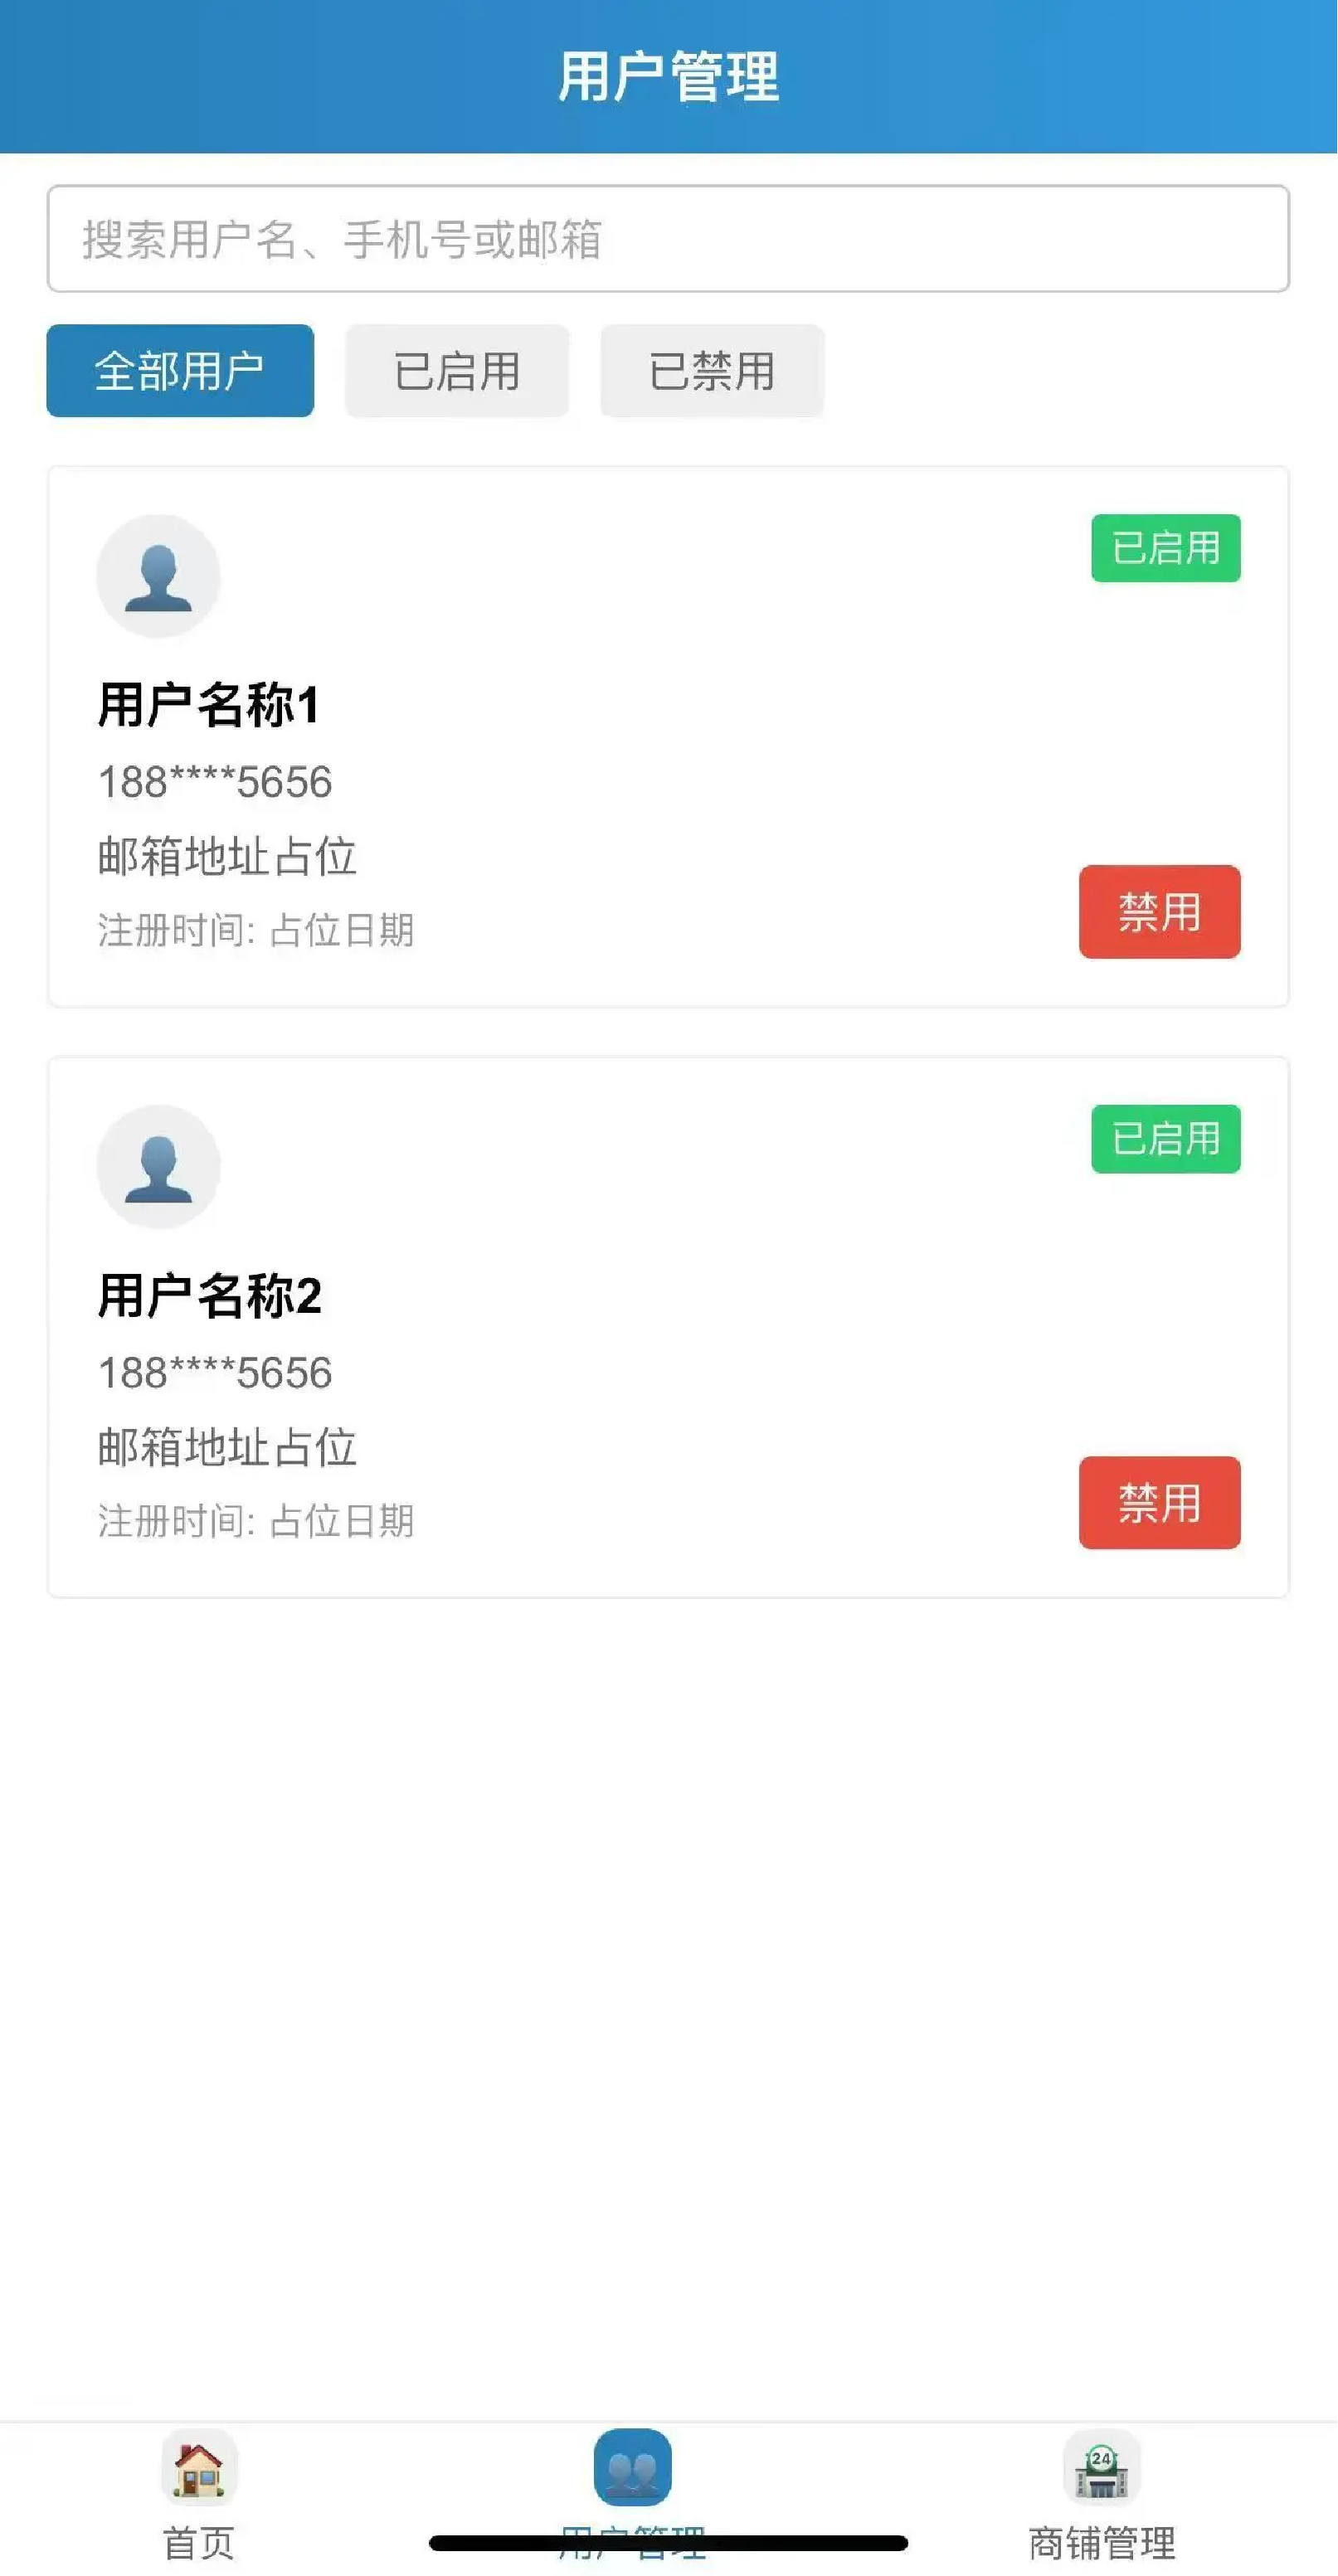
\includegraphics[width=0.8\linewidth]{figures/frontend/img8}
    \end{minipage}

    \hspace*{-1.5cm}

    \caption{管理员首页 \& 用户管理页面}
    \label{fig:interfaces}
\end{figure}

% 章节结束
